% file thesis.tex
% Master Document

\documentclass[a4paper,oneside,11pt]{book} %twoside,draft,openright]
\tolerance=1000  % all 3 of these commands make LaTeX less fussy about what
\hbadness=10000  % is a ``good'' length/width/height of a page
\raggedbottom

% For Margins
\usepackage{a4}
\usepackage{anysize}
%{left}{right}{top}{bottom}
%\marginsize{38mm}{25mm}{25mm}{25mm} % For print
\marginsize{31.5mm}{31.5mm}{25mm}{25mm} % For web

\usepackage{ifxetex}

\usepackage{array}
\usepackage{colortbl}
\usepackage{multirow}

% Makes the text looks a little nicer
\ifxetex
    \usepackage[table,hyperref]{xcolor}

    %for use with XeTeX
    \usepackage{fontspec}
    \usepackage{xunicode}
    \usepackage{xltxtra}

    \defaultfontfeatures{Mapping=tex-text} % converts LaTeX specials (``quotes'' --- dashes etc.) to unicode

    \setmainfont[Scale=1.075,Ligatures={Common},Numbers={Lining}]{Adobe Garamond Pro}
    %\setmainfont[Scale=1.075,Ligatures={Common},Numbers={Lining}]{Adobe Caslon Pro}
    %\setmainfont[Scale=1.075,Ligatures={Common},Numbers={Lining}]{Minion Pro}

    %Look at Neosan for headings

    %\setromanfont [Ligatures={Common,Rare},Numbers={OldStyle}]{Adobe Garamond Pro}
    %\setmonofont[Scale=0.8]{Monaco}
    %\setsansfont[Scale=0.9]{Optima Regular}
\else
    \usepackage[table,fixpdftex,hyperref]{xcolor}

    \usepackage[ansinew]{inputenc}

    % Makes copy and paste work better ie ligatures get converted
    \usepackage{cmap}
    \usepackage{mmap}
    \usepackage[protrusion=true,expansion=true]{microtype}

    % Use a nice Adobe font
    % used instructions from: http://umrg.uwaterloo.ca/cpoile/LaTeX
    \usepackage[LY1]{fontenc}
    %\usepackage[ansinew]{inputenc}
    %\usepackage[scaled=1.05,lining]{GaramondPro} % [oldstyle] for different number style
    % can use \textos{1234} or \textln{5678} to change how the numbers are displayed
\fi

\usepackage[font=small,format=hang,labelfont=bf,up,up]{caption} % fancy captions

% Removed the following because it doesn't work very well
%\usepackage[notlot,notlof]{tocbibind} % Adds the ToC, Bib, etc to the table of contents.
\usepackage[titles]{tocloft} % Allows the table of contents to be altered easily

\usepackage{subfig}
\usepackage{graphicx}

\usepackage{titling} % Allows the title page vars to be reused

\usepackage{setspace} %double spacing for text, single for captions,
		      	   %footnotes, etc.
%\usepackage{draft} %draft option - doesn't put full figures in -
		    % useful when editing

\usepackage{needspace}

% Makes fancy footers/headers on the pages
\usepackage{fancyhdr}

\usepackage{savefnmark} % For reusing footnotes

% Change the font for section headings
\usepackage{sectsty}
\allsectionsfont{\sffamily}

\usepackage{fncychap} % fancy Chapters headings

% Hacked version of Sonny
\makeatletter
  \ChNameVar {\sffamily\Huge}           % sets the style for name
  \ChNumVar  {\sffamily\Huge}           % sets the style for digit
  \ChTitleVar{\sffamily\Huge\bfseries}  % sets the style for title
  \ChRuleWidth{0.5pt}
  %\ChNameUpperCase           % Make name uppercase

  \renewcommand{\DOCH}{%     % formats the chapter name and number.
    \raggedright
    \CNV\FmN{\@chapapp \space \thechapter}
    \par\nobreak}

  \renewcommand{\DOTI}[1]{%  % formats the chapter title for \chapter
    \raggedright
    \CTV\FmTi{#1}\par\nobreak
    \vskip -1\baselineskip\vskip 10pt\mghrulefill{\RW}\par\nobreak
    \vskip 40\p@}

  \renewcommand{\DOTIS}[1]{%  % formats the chapter title for \chapter*
    \raggedright
    \CTV\FmTi{#1}\par\nobreak
    \vskip -1\baselineskip\vskip 10pt\mghrulefill{\RW}\par\nobreak
    \vskip 20\p@}

\makeatother

% Allow for multiple bibs
\usepackage{multibib}
\newcites{A,B}{Related Publications,Other Publications}

\usepackage{enumitem} % Customise lists
\setdescription{leftmargin=1em} % Make the lists less indented

% Adds extra PDF metadata
\usepackage{hyperxmp}

%for PDF features (last imported package, for maximum capability)
\ifxetex
    \usepackage[unicode,xetex,pdfpagelabels,pagebackref]{hyperref} % For the bookmark/hyperlinks
\else
    \usepackage[unicode,pdftex,pdfpagelabels,pagebackref]{hyperref} % For the bookmark/hyperlinks
\fi

% for the algorithm
\usepackage{algorithm}
\usepackage{algorithmic}

\usepackage[all]{hypcap} % Changes figure links to the top of figures, not the captions

% *************************** Metadata *********************************

    % Perhaps, "The Impact of Highly Interactive Workloads on Video-on-Demand Systems"
    % The Impact of Highly Interactive Workloads on Content Distribution Networks
\title{The Impact of Highly Interactive Workloads on Video-on-Demand Systems}
\author{Andrew Brampton B.Sc (Hons)}
\date{September 2008}

\hypersetup{%
    pdftitle={\thetitle},
    pdfauthor={\theauthor},
    pdfsubject={},
    pdfkeywords={Interactive, Video-on-demand, Multimedia, Workloads, Characterisation},
    pdfcopyright={Copyright (C) 2008, Andrew Brampton},
%
    plainpages=false,
    bookmarksnumbered=true,
    pdfstartview={FitV}, % Full screen vertical
    colorlinks={false},  % No color links
    pdfborder={0 0 0},   % No borders around links
%
    pdfcreator={XeTeX},%
%    pdfproducer={XeTeX}%
%
%    colorlinks={true},  % We specify color links, but set them to black, so we don't get boxes around each link
%    linkcolor={black},  % Color for normal internal links.
%    anchorcolor={black},% Color for anchor text.
%    citecolor={black},  % Color for bibliographical citations in text.
%    filecolor={black},  % Color for URLs which open local files.
%    menucolor={black},  % Color for Acrobat menu items.
%    urlcolor={black},   % Color for linked URLs.
}

% **************************** Macros **********************************

\newcommand{\todo}[1]{
    %\fcolorbox{red}{white}{
    \fbox{
        \color{red}
        \small
        \sf TODO: #1
    }
}

% **************************** Some custom table stuff Macros

%\cellw{width}{text}
\newcommand{\cellw}[2]{%
    \begin{minipage}[c]{#1}
        \begin{center}#2\end{center}
    \end{minipage}%
}

%\cellxyw{cols}{rows}{width}{opt}{text}
\newcommand{\cellxyw}[5]{
\ifx1#1 % One col
    \ifx1#2 % One col - One row
        #5
    \else % One col - Multi rows
        \multirow{#2}{*}{%
            \cellw{#3}{#5}
        }
    \fi
\else % Multi cols
    \ifx1#2 % Multi cols - One row
        \multicolumn{#1}{>{\columncolor{\RowColorName}}#4}{%
            \cellw{#3}{#5}
        }
    \else % Multi cols - Multi rows
        \multicolumn{#1}{>{\columncolor{\RowColorName}}#4}{%
            \multirow{#2}{*}{%
                \cellw{#3}{#5}
            }
        }
    \fi
\fi
}

\newcommand{\cellxy}[3]{\cellxyw{#1}{#2}{#1\tablecolwidth}{c}{#3}}
\newcommand{\cellbxy}[3]{\cellxyw{#1}{#2}{#1\tablecolwidth}{c}{\textbf{#3}}}

\newcommand{\cellendxy}[3]{\cellxyw{#1}{#2}{#1\tablecolwidth}{c|}{#3}}
\newcommand{\cellendbxy}[3]{\cellxyw{#1}{#2}{#1\tablecolwidth}{c|}{\textbf{#3}}}

\newcommand{\setrowcolor}[1]{\noalign{\gdef\RowColorName{#1}}\rowcolor{\RowColorName}}

\definecolor{TableRowHead}{rgb}{0.52734375,0.63671875,1} %87a3ff
\definecolor{TableRowA}{rgb}{1,1,1}
\definecolor{TableRowB}{rgb}{0.858,0.898,0.945} %dbe5f1

\newlength{\tablecolwidth}
%\setlength{\tabcolsep}{2pt} % horz spacing
%\setlength{\extrarowheight}{2pt} % spacing above cell
\setlength{\arrayrulewidth}{1pt}

% *****************************************************

% Puts angle brackets around some text
\newcommand{\bracket}[1]{\textless #1\textgreater}

% Set the section number depth
\setcounter{secnumdepth}{3}
\setcounter{tocdepth}{3}
%
\renewcommand{\cftsecindent}{1 em}
%\renewcommand{\cftsecnumwidth}{1.9 em}

\renewcommand{\cftsubsecindent}{2 em}
%\renewcommand{\cftsubsecnumwidth}{2.8 em}

\renewcommand{\cftsubsubsecindent}{3 em}
%\renewcommand{\cftsubsubsecnumwidth}{3.2 em}

% Configure \autoref
% http://osdir.com/ml/emacs.auctex.general/2005-11/msg00093.html
% http://www.latex-community.org/viewtopic.php?f=4&t=334
\def\chapterautorefname{Chapter}
\def\sectionautorefname{Section}
\def\subsectionautorefname{Subsection}
\def\subsubsectionautorefname{Subsection}
\def\figureautorefname{Figure}
\def\subfigureautorefname{Figure}
\def\tableautorefname{Table}
\def\algorithmautorefname{Algorithm}

\newcommand{\sth}[0]{\textsuperscript{th}\space}
\newcommand{\st}[0]{\textsuperscript{st}\space}
\newcommand{\nd}[0]{\textsuperscript{nd}\space}
\newcommand{\rd}[0]{\textsuperscript{rd}\space}


% ******************** Include Only These Files ************************
%\includeonly{}
%\includeonly{title,abstract,acknowledgment}
\includeonly{title,abstract,acknowledgment,publications,intro,background,experiment,evaluation,improve,conclusion,bibliography}
%\includeonly{background, bibliography}
%\includeonly{intro}
%\includeonly{experiment}


%Defines the headers of the page
\pagestyle{fancy}
\renewcommand{\chaptermark}[1]{\markboth{\chaptername\ \thechapter:\,\ #1}{}}
\renewcommand{\sectionmark}[1]{\markright{\,\ #1}}

% fancyhdr settings
\headheight 16.60005pt % Set to remove warnings
\fancyhead{}
\fancyhead[L]{\rm\leftmark}
\fancyhead[R]{\rm\rightmark}

\fancyfoot{}
\fancyfoot[C]{\thepage}

%%%%%%%%%%%%%%%%%%%%%%%%%%%%%%%%%%%%%%%%%%%%%%%%%%%%%%%%%%%%%%%%%%%%%%%%%%%
%%%%%%%%%%%%%%%%      end of preamble and start of document     %%%%%%%%%%%
%%%%%%%%%%%%%%%%%%%%%%%%%%%%%%%%%%%%%%%%%%%%%%%%%%%%%%%%%%%%%%%%%%%%%%%%%%%
\begin{document}

\frontmatter
    \newpage
\thispagestyle{empty}
\setcounter{page}{0} % Hack to remove dup page i message

% ******* Title page *******
% **************************

\vspace*{0.5cm}

\begin{center}
    % Perhaps, "The Impact of Highly Interactive Workloads on Video-on-Demand Systems"
    % The Impact of Highly Interactive Workloads on Content Distribution Networks
    {\Huge\bfseries \thetitle \\}
    \vspace{1.5cm}
    {\huge \theauthor \\}

    \vspace{1.5cm}

    {\LARGE Thesis submitted for the degree of\\Doctor of Philosophy\\}

    \vspace{1.5cm}

    
\includegraphics[height=6.5cm]{./lancs-logo}

    {\LARGE
    Computing Department\\
    Lancaster University\\
    \vspace{1cm}
    \thedate
}
\end{center}

%\newcommand{\HRule}{\rule{\linewidth}{0.5mm}}
%
%\begin{titlepage}
%
%\begin{center}
%
%% Upper part of the page
%
\includegraphics[width=0.15\textwidth]{./lancs-logo}\\[1cm]
%
%\textsc{\LARGE Computing Department\\Lancaster University}\\[1.5cm]
%
%\textsc{\Large Thesis submitted for the Degree of Doctor of Philosophy}\\[0.5cm]
%
%% Title
%\HRule \\[0.4cm]
%{ \huge \bfseries \thetitle}\\[0.4cm]
%\HRule \\[1.5cm]
%
%% Author and supervisor
%\begin{minipage}{0.4\textwidth}
%    \begin{flushleft} \large
%        \emph{Author:}\\
%        \theauthor
%    \end{flushleft}
%\end{minipage}
%
%\begin{minipage}{0.4\textwidth}
%    \begin{flushright} \large
%        \emph{Supervisor:} \\
%        Prof. Laurent Mathy
%        Dr. Nicholas Race
%    \end{flushright}
%\end{minipage}
%
%\vfill
%
%\end{center}
%
%\end{titlepage}

% Reset the numbering so the title page isn't counted
\newpage
\setcounter{page}{1} 

\doublespacing
\pagestyle{plain}

    

%\begin{abstract}
%specific program, how I approached the problem,
%not focused enough, What I've done, why, what I got out of it
%what I've done, what I've achieved, and why? Make it exciting
%If you don't understand the topic after the abstract, then you have problems
%If you read the introduction, and you still don't understand you have major problems
%must reflect my vision, and what I've done
%few bullet points, what is important, sentences then paragraph – top down
%what is important to be said
%gun to my head, 30seconds to impress them
%read some other thesis
%original and significant contribution
%\end{abstract}

%\begin{itemize}
%  \item Start-to-finish model isn't used.
%  \item High levels of interactive observed, aided by bookmarks
%  \item Not all of the video is equally popular, they are ranked based on power-law distributions.
%  \item Caused hotspots, which normally start at a bookmark
%  \item Techniques to dynamically move bookmark as well as work out the corresponding length
%  \item The high interactive loses us some predictability. However the order in which they view bookmarks is predictable
%  \item All of this has been modelled
%\end{itemize}

\phantomsection
\addcontentsline{toc}{chapter}{Abstract}

%\chapter{Abstract}
%\begin{abstract}
% No more than 300 words

\begin{center}
{\LARGE\bfseries \thetitle\\}
{\Large\bfseries \theauthor\\}
{\large Thesis submitted for the degree of Doctor of Philosophy\\
\thedate}
\end{center}

\section*{Abstract}

The traditional start-to-finish playback model is not suitable for all modern interactive video streams. Users expect support for higher levels of interactivity such as fast forward and rewind or the ability to arbitrary seek within their media quickly and efficiently. By conducting user studies we have observed start-to-finish is not applicable to many genres of video, and that different playback models fit better. We discuss how existing delivery techniques are impacted by these new observations.

Novel interactive controls such as bookmarks have also highly impacted user behaviour. This has lead to the segments within the media being accessed in a uneven fashion, causing hotspots of interest to form; areas with orders of magnitudes more viewers than others. These hotspots typically began at the beginning of a bookmark, however not always, which lead us to design a dynamic bookmark positioning algorithm. As well as their position, determining the hotspot's length can be beneficial. This aids in autonomic techniques such as replication and pre-fetching as well as allowing the users to find what they want quicker.

Under high level of interactivity, delivery techniques are less efficient due to the unpredictability of the users. We however developed techniques which restore some of this predictability, allowing clients or servers to predict future actions based on past user actions. These technique proves exceeding useful for pre-fetching which reduces seek latencies for client and can reduce load on servers. However knowledge of past user activities need to be gathered from network, thus we develop techniques to do this in a distributed manner.


%\section{The Pitch}

%Media streaming is increasingly being used online, with CDNs being deployed to handle the sheer volume of requests. As such systems are becoming commonplace, users are expecting improved functionality, for example interactive controls. This is increasingly difficult to provide with differing content types, and when existing CDN techniques do not work well under interactive workloads. I show that simple interactive workloads are exceedingly different from traditionally discovered workloads (such as the start-to-finish model) and that these new workloads add a degree of unpredictability. However by adding simple interactive features such as bookmarks, and observing past user behaviour, it is possible to gain some insight into what the user will watch, and in what order. Techniques have been developed to gather the past user actions in a distributed manner~\footnote{Distributed techniques will be developed soon} and to exploit this data to improve playback for all users under an interactive scenario.

%\end{abstract} 

\chapter*{Declaration}

\large

This thesis is a presentation of my original research work. No part of this thesis has been submitted
elsewhere for any other degree or qualification. All work is my own unless otherwise
stated. The work was carried out under the guidance of Laurent Mathy and Nicholas Race, at Lancaster University's Computing Department.

\vspace{3.5cm}

\begin{center}
\begin{tabular}{lll}
  \rule[-0.5em]{7cm}{0.5pt} & \hspace{1cm} & 30\sth September 2008  \\
  Andrew Brampton & & Date \\
\end{tabular}
\end{center}

\vspace{3.5cm}

\noindent
Copyright \copyright 2008 by Andrew Brampton.\\
``The copyright of this thesis rests with the author. No quotations should be published
or information and results derived from this thesis without acknowledgement.''

    \chapter{Acknowledgments}
%\addcontentsline{toc}{chapter} {\protect\numberline{Acknowledgments\hspace{-96pt}}}

%The past few years have been some of the hardest of my live. Writing a P
Writing my thesis has been one of the hardest tasks in my life, and I couldn't have completed it without the support from my friends, family and the computing department. 

Firstly, I would like to thank my two supervisors, Laurent Mathy and Nicholas Race. They have kept me on the straight and narrow, always pointing me in the right direction. I would like to especially thank Laurent, for his tough supervision, which at times seemed harsh, but on reflection pushed me to become a far better researcher. I am also appreciative of Michael Fry's guidance, who in the last year has infused me with new ideas, and direction.

%I would like to thank my friends for  when I needed them, and sometimes when I didn't.
My friends have been there for me through my university life and constantly offering distractions from my studies, sometimes when I needed it, and others times when I didn't! Nevertheless, their backing has been greatly appreciated, especially my housemates, who have offered a good sounding board when I needed to work through a problem. A special thank you should go to Nicola, who in the last few weeks has greatly helped with proofreading of my thesis.

Finally, I would like to thank my parents and brother for being supportive during my PhD journey, and there for me when I needed them.

%, even if they have never quite understood what I've been doing.


%The Engineering and Physical Sciences Research Council (EPSRC) for funding

%\begin{itemize}
%    \item Academic People
%    \item Friends \& Family
%\end{itemize}

\singlespacing
\vspace*{1cm}
\begin{center}
    \it ``Time waits for no one'' \hspace*{0.5cm}
\end{center}
\begin{flushright}
    \small The Rolling Stones - 1974\hspace*{3cm}
\end{flushright}
\doublespacing

%"Time waits for no man" is originally a quote from a section by Death in the famous medieval play "Everyman" regarding certainty. The original line is in middle English is "For wete you well the tyde abydeth no man" but most schlars attribute this 'tyde' as a statement of time, as in Christmastide, etc. rather than a reference to the tides themselves. However, misunderstanding of the older form of language have led to the the common day phrase 'time and the tides wait for no man' which can be found in several literary allusions as well as movies such as Shakespeare in Love.

    
\phantomsection\addcontentsline{toc}{chapter}{Publications}

% Used to force the order of the citations
\nociteA{brampton2007cui,brampton2008cew,macquire2008acf}
\bibliographystyleA{unsrt}
\bibliographyA{related}

\nociteB{brampton2005sdh,macquire2006pas,macquire2006asd,brampton2006sdh,rai2007pmp}
\bibliographystyleB{unsrt}
\bibliographyB{other}


    \singlespacing

\chapter{Thesis Plan}
\label{chap:plan}

\begin{itemize}
    \item Introduction
    \begin{itemize}
        \item Streaming is popular on the internet
        \item Streaming is bandwidth and latency intense
        \item CDNs/Streaming Protocols are used to allow for best streaming performance
        \item These assume start-to-finish model

        \item Users want more than start-to-finish
        \item VCR style controls are used
        \item More novel interactivity controls such as bookmarks could also be used
        \item Current CDNs/Streaming protocols are not optimised for these interactive workloads
    \end{itemize}

    \item Background

    \begin{itemize}%
        \item Previous characterisations of Access Patterns
        \begin{itemize}
            \item Video-on-Demand
            \begin{itemize}
                \item Popularity
                \item Popularity Over Time / Recommendations
                \item Session duration
                \item Interactivity
                \item Popularity Within Content
            \end{itemize}
            \item Live Streaming
            \begin{itemize}
    				\item Popularity
    				\item Time-of-day
    				\item Session duration
    				\item Interactivity
            \end{itemize}
        \end{itemize}

        \item Discussion on Interactivity and how it breaks streaming
        \begin{itemize}
            \item Introduction
            \item Push/Pull Techniques~\footnote{incorporating Andy's Hybrid work.}\saveFN\andy\
            \item Hybrid concepts~\useFN\andy\
        \end{itemize}

        \item Papers about VoD systems, such as YouTube, and M\$'s
        \begin{itemize}
            \item Overview
            \item Describe what's typical on these services
            \item Describe what problems they have
        \end{itemize}

    \end{itemize}

    \item Experiment
    \begin{itemize}
        \item User Study setup
        \item Tools developed (P2P Simulator, FLVTool++)
    \end{itemize}

    \item Evaluation (and modelling)
    \begin{itemize}
        \item Interactions
        \item Seek Distance
        \item Popularity
        \item Longevity
        \item Session Lengths
        \item Inter-seek Times
        \item Sequence
        \item Hotspot Length
    \end{itemize}

    \item Approaches to improve interactivity
    \begin{itemize}
        \item Bookmark Creation and Moving Bookmarks
        \item Hotspot detection
        \item Predictive pre-fetching
        \item Techniques to support these in a distributed way~\footnote{80\% done}
        \item Hybrid Streaming Techniques~\useFN\andy\
    \end{itemize}

    \item Conclusions
    \begin{itemize}
        \item Thesis Contributions
        \item Future Work
        \item Summary
    \end{itemize}
    
%    \item Extras (not currently included)~\footnote{Needs starting}
%    \begin{itemize}
%            \item Distributed pre-fetching, how can my miss be your hit?
%            \item Repeat visits to the worldcup site
%
%            \item Check if my results are ``fetch-at-most-one'' or not?
%
%            \item Look at probability of two events happening next to each other. ie 2 forward jumps, or 2 pauses, or forward jump then backwards jump.
%
%            \item Look at ``spurts'' of interactivity requests. ie do they happen uniformly across the session, or mostly in one go.
%
%            \item Look at CDF of \# of interactive request per user
%    \end{itemize}

\end{itemize} 

\onehalfspacing
    \renewcommand\contentsname{Table of Contents}
    \phantomsection\addcontentsline{toc}{chapter}{\contentsname}
    \tableofcontents

    \newpage
    \listoffigures% \addcontentsline{toc}{chapter}{List of Figures}

    \newpage
    \listoftables% \addcontentsline{toc}{chapter}{List of Tables}

\doublespacing
%\onehalfspacing
%\singlespacing

\mainmatter
    \pagestyle{fancy}

    \chapter{Introduction}
\label{chap:intro}

% Step back
% Don't lose site of the genre
% What's been done, what hasn't been done, whats the context of all this,
% How does Hybrid fit in?
% Don't claim I've solved world problems
% Why you should carry on reading
% last para "Why this is signatificate and new?". This is a signatifant statement.

%\begin{itemize}
%  \item Streaming is popular on the internet
%  \item Streaming is bandwidth and latency intense
%  \item CDNs/Streaming Protocols are used to allow for best streaming performance
%  \item These assume start-to-finish model
%
%  \item I show that users want more than start-to-finish
%  \item When given the option VCR style controls are used
%  \item More novel interactivity controls such as bookmarks could also be used
%  \item Current CDNs/Streaming protocols are not optimised for these interactive workloads
%  \item Hybrid techiniques can be employed
%
%  \item Do I talk about what I did?
%
%\end{itemize}

% Nic has read

In recent years, the distribution of multimedia rich content has become increasingly popular via the internet. Websites offer a range of media, from short user generated clips to high definition feature films. This content typically has strict delivery requirements, needed for optimal playback. The requirements typically include high bandwidth connections and demands low latencies and low jitter.

Many techniques are employed by both client and server to ensure smooth delivery and to minimise operational costs. These techniques include (but are not limited to) pre-fetching, tree-based distribution, and deploying full content distribution networks (CDNs). Generally, these techniques assume that the user consumes the content conforming to particular usage models. The most commonly assumed models are the classic \emph{start-to-finish} model and an extension of this, the \emph{start-to-end} model. With the former model, users will start playback at the beginning of the content and continue until the very end, whereas the latter model assumes that the users stop playback before the end.

As such systems evolve, users expect more control over the playback of their content, and thus improved functionality. For example, VCR-like controls are already common; fast-forward, rewind, pause and resume. More novel interactivity controls are beginning to appear, for example, bookmarks, which give the user the ability to seek directly to a point of interest within the content, such as a chapter or an event.

Offering services which provide a high level of interactive control creates new challenges for traditional delivery mechanisms. For example, conventional network and application-level multicast is not suitable for providing interactivity. Conversely, simple client-server mechanisms work well under high interactivity, however, they can not easily scale to offer a large number of users these services. Regardless of delivery, there are additional problems such as delay caused by start-up or seek latency, as well as the unpredictable workload placed upon the servers.

Nevertheless, there are numerous commercial video-on-demand services which offer varying degrees of interactivity. Thus far, these systems use a brute-force approach, deploying large scale CDNs to satisfy the needs of their users. This thesis will explain how these existing deployments work, and highlight their flaws. We will then continue by discussing how these techniques can be improved to support interactivity, as well as develop some new techniques.

\section{Research Contributions}

%\begin{itemize}
%  \item Run two experiments with novel interactivity controls
%  \item Analysis these experiments and show a departure from the classic start-to-finish
%  \item Generate new models from the user's behaviour
%  \item Show that we can exploit these new models
%  \item Show how these new models can be used by hybrid delivery mechanisms
%\end{itemize}

This thesis presents through experimentation new user behaviour models, more applicable to highly interactive content. These models can aid in simulation and development of new techniques for efficient, quick and cheap delivery of content to the user. The models were derived from data obtained by an experimental Video-on-Demand (VoD) website which we designed and deployed. In addition to generic VCR-like features, this custom built VoD application provided advanced interactivity features such as bookmarking. Over a twelve month period more than 1000 unique users were observed accessing a selection of 88 video files. These videos included the entire 2006 FIFA World Cup and the 2007 Eurovision song contest.

Through detailed analysis of the data, common usage models were characterised, such as object popularity, session duration, and other standard metrics. It was observed that when users were offered additional interactive controls, the content was no longer consumed based on the \emph{start-to-end} model. To aid in characterising this novel user behaviour, additional interactive metrics were developed, which better explained this highly interactive system. These include models for how bookmarks are used, as well as models relating to an emergent property, \emph{hotspots}. These \emph{hotspots} are areas of particular interest within the video in which users often choose to watch (and replay) small segments of the full video, in a complete departure from the classic models. While the behaviour observed may be specific to the content used within the experiments, the results may be of general interest, and relevant to other genres of video with popular highlights (e.g., educational, entertainment, news, \emph{etc.}).

This thesis will discuss how current delivery techniques are not designed to handle such levels of interactivity. Understanding these new models can lead to new techniques to improve the delivery of highly interactive media. For example, the actions of a user may now be predicted based on past users. Also, distributed techniques were developed to detect the location of \emph{hotspots} automatically. Knowing the position of \emph{hotspots} presents new opportunities for caching and replication techniques which did not previously exist with less interactive media. Following from this, new hybrid delivery techniques are explored, which use a combination of established delivery protocols. Hybrid delivery allows for quick, efficient, and cheap delivery of content, while offering the user high levels of interactivity not available with existing delivery systems.

%These includes the analysis of how bookmarks were used, as well as the ability to predict the users next action. , and the abilities to predict which boo

\section{Thesis Structure}

After this chapter, this thesis is organised into five chapters. The chapter immediately following this introductory chapter provides background of existing characteristics models in the areas of live and stored streaming media, and their deficiency in modelling interactive behaviour. The background is continued by explaining how interactive media can be delivery, and the problems with this, and then concluding with a discussion of existing video-on-demand deployments and the problems they face.

\autoref{chap:experiment} describes the design of a video-on-demand system we used to experiment and evaluate new interactive video concepts. This is followed by \autoref{chap:evaluation}, which discusses the results obtained from our experiments, with details on characterising the users behaviour and how these can be modelled for future simulations. The evaluation also contains discussion of the implication these new interactive models have on the design of new systems. \autoref{chap:new_techiques} builds on the results obtained, and discusses ideas which can improve the delivery of interactive media for both the consumer and distributer. This includes dynamic bookmark placement, pre-fetching and a hybrid delivery technique.

This thesis is concluded with \autoref{chap:conclusion} which gives a overview of the work presented in this thesis. The conclusion also suggest future directions for this research. 
    \chapter{Background \& Related Work}
\label{chap:background}

%Nic has read

%\begin{itemize}%
%    \item Previous characterisations of Access Patterns
%        \item Static Content
%        \item Video-on-Demand
%            \item Popularity
%            \item Popularity Over Time / Recommendations
%            \item Session duration
%            \item Interactivity
%            \item Popularity Within Content

%        \item Live Streaming
%				\item Popularity
%				\item Time-of-day
%				\item Session duration
%				\item Interactivity

%    \item Discussion on Interactivity and how it breaks streaming
%        \item Introduction
%        \item Push/Pull Techniques
%        \item Hybrid concepts

%    \item Papers about VoD systems, such as YouTube, and M\$'s
%        \item Delivery techniques
%        \item Caching techniques
%        \item VoD Websites (YouTube, etc)
%        \item Overview
%        \item Describe what's typical on these services
%        \item Describe what problems they have
%

%\end{itemize}

%\item Papers about VoD systems, such as YouTube, and M\$'s
%\begin{itemize}
%    \item Overview
%    \item Describe what's typical on these services
%    \item Describe what problems they have
%\end{itemize}

% YouTube paper (I tube, you tube, everybody tubes: analyzing the world's largest user generated content video system)
% M$ VoD Paper (Can Internet Video-on-Demand Be Profitable?)
% Chinese Telecom paper (

%\todo{Explain the focus of this research, and how interactive apps do exist, but what are their limitations}


The focus of this thesis is understanding how video-on-demand (VoD) systems operate under highly interactive workloads. Once a firm understanding of this is achieved, then new techniques can be designed to help improve performance in such systems. Therefore, the first section of this chapter aims to explain how currently deployed VoD systems work. Special attention is paid to which interactive features these systems already provide, as well as their limitations in providing advanced interactivity. This covers systems such as the incredibly popular YouTube~\cite{youtube}, serving low quality short video clips via a content distribution network (CDN), to systems such as BBC iPlayer~\cite{iplayer}, a hybrid peer-to-peer CDN platform offing high quality professional content.

Later, to understand exactly how workloads are analysed, \autoref{sect:characterisations}, provides a detailed overview of how existing characterisation studies have try to explain and model user behaviour. Modelling behaviour is very important for designing video-on-demand mechanisms, for example, understanding the popularity of objects helps to make caching and replication decisions. Most of the existing research on characterising user behaviour has either ignored, or not experienced high levels of interactivity. This is counter to the results displayed later in this thesis. As such, the review of previous work is discussed in the context of interactive workloads, where applicable. This helps motivate the experiments evaluated in \autoref{chap:evaluation}, as well as providing a solid ground to understand the problems with interactivity.

%Finally, \autoref{sect:deliverinteract} expands on the previous two section by highlighting what related research has gone into creating scalable and efficient systems for providing interactivity. This forms the background knowledge for \autoref{chap:new_techiques}.

\section{Deployed Video-on-Demand Systems}
\label{sect:video-on-demand}
%    The content length is shortened by two orders of magnitude and so is the production time.
%     Wired magazine refers to this small-sized content pop culture as �bite-size bits for high-speed munching� [34].
%    [34] N. Miller. Manifesto for a New Age. Wired Magazine, March 2007

    There are multiple systems now in place, which allow users to watch videos when they want, how they want. There is an abundance of content available, ranging from short funny video clips, to long feature movies, and everything in between. This has been driven by incredible demand, causing new video-on-demand (VoD) systems to appear, almost daily, to serve different niches. To keep up with demands, these videos are no longer just made by professionals. Anyone with a cheap camcorder or webcam can become famous for 5~minutes. Wired magazine refers to this as ``bite-size bits for high-speed munching''~\cite{miller2008mfa}.

    As VoD is becoming more ubiquitous, users are expecting more features. One such feature is interactivity, the ability to pause, resume, and seek within the content. Many of these VoD systems are offering interactive features, however, each with their own limitations. For example, some can only offer interactivity by forcing the user to download the full video first. If they do allow interactivity via streaming, then the systems seem slow or sluggish.

    This section highlights the main classes of VoD applications, and well as how they work. Their interactivity features are discussed in detail, as well as their flaws. At the end of this section, there is a summary of all solutions, giving a quick overview of what is out there, and how it operates.

\subsection{Flash-based Sites}
\label{sect:ugc}
%Checked by Nic

\begin{table}
\center
\begin{tabular}{|rccc|}
\hline
\setrowcolor{TableRowHead}
                                          & YouTube &   Dailymotion  &    Metacafe    \\
\hline
\setrowcolor{TableRowA}
  Unique Visitors ($\times 10^6$/month)   & 70      & 10             & 10             \\
\setrowcolor{TableRowB}
  Videos Watched ($\times 10^6$/day)      & 100     & 25             & 15             \\
\setrowcolor{TableRowA}
  Alexa Site Rank (Feb '08)               & 3       & 31             & 179            \\
\setrowcolor{TableRowB}
  Stored Videos (2006)                    & 45 TB   & \emph{unknown} & \emph{unknown} \\
\setrowcolor{TableRowA}
  Stored Videos (2007)                    & 357 TB  & \emph{unknown} & \emph{unknown} \\
\hline
\end{tabular}
\caption[Overview of the most popular video sharing websites]{Overview of the most popular video sharing websites, adapted from~\cite{saxena2008avs,cheng2007uci}}
\label{tab:videosites}
\end{table}

    A big push in storing videos online has been the creation of \emph{user generated content} (UGC) websites such as YouTube~\cite{youtube}, Dailymotion~\cite{dailymotion}, Metacafe~\cite{metacafe} as well as many more~\cite{msnvideo,googlevideo,hulu,myspacetv}. The most popular of these sites, YouTube, was founded in 2005. Despite only being three years old, it is now the 3\rd most popular site on the internet, illustrating how popular these sites are. \autoref{tab:videosites} gives a brief overview of the most commonly used UGC sites' popularity, as well as how many videos are viewed and stored on these services.

    These Web 2.0\footnote{Web 2.0 is a term to describe a new generation of websites, where the site's value comes from the users who participate.} websites allow users to upload their own videos for others to watch freely. Once uploaded, other users can begin tagging~\cite{ames2007wtm}, rating and commenting on each video. Users may also share their favorite videos with their friends, allowing the video to quickly disseminate through a video sharing social network.

    Typically the content on the sites is short low quality clips. A study of YouTube by Cheng~\emph{et~al.} found that 97.8\% of all videos were shorter than 10 minutes~\cite{cheng2007uci}. This is due to a limit imposed by YouTube, that regular users may only upload videos 10 minutes or shorter. A different study found that the mean viewing length was 4.15~minutes with a median of 3.33~minutes~\cite{gill2007ytc}. There is a small group of authorized users who may upload longer videos, which includes content such as documentaries or lectures. These short length videos are not representative of all sites; an analysis of MSN Video found that many of the videos were a lot longer than YouTube, however no exact figures or distributions of lengths were offered~\cite{huang2007civ}.

    These sites typically use \emph{pseudo-streaming} (or sometimes called \emph{progressive download}) techniques~\cite{guo2005amw}. This is where a media file is downloaded using general file downloading techniques, but as it downloads it is also played. As a true streaming protocol is not used, many features are lacking, for example, the rate the server transmission the file will not be synchronised with the playback rate. This may cause the stream to be received faster or slower than required. Additionally controls such as pause or seeking are not easily available.

    The most common example of \emph{pseudo-streaming} involves a combination of an Adobe Flash player and HTTP downloading. A web page contains a Flash video player which requests a Flash video file (FLV) from the HTTP server. The Flash file is downloaded just like any other file would be via HTTP. As the file downloads, the Flash player can begin playback.

    Flash video was chosen due to its widespread deployment. For example, in 2000, the Flash player was distributed with AOL, Netscape and Internet Explorer browsers. Later, in 2002, the Flash player came pre-installed with Windows XP. This lead to an unverified claim that Flash Player had an install-base of roughly 92\% of all internet users~\cite{wiki_flash}.

    Flash video can be compressed using various encodings. On YouTube, the video is encoded with the Sorenson Spark H.263 codec, with a resolution of 320x240 at 25 frames per second~\cite{cheng2007uci}. This creates videos which have a bitrate of around 330~kbps. However, YouTube is at the lower end of quality, compared to other UGC sites. Due to home broadband becoming more ubiquitous, there has been greater demand for higher quality videos. For example, in February 2008, Dailymotion announced that it would begin streaming at the high-definition resolution of 720p~(1280x720)~\cite{lowensohn2008dgh}, requiring at least 8-16~Mbps bitrate streams.

\begin{figure}[t]
    \centering

    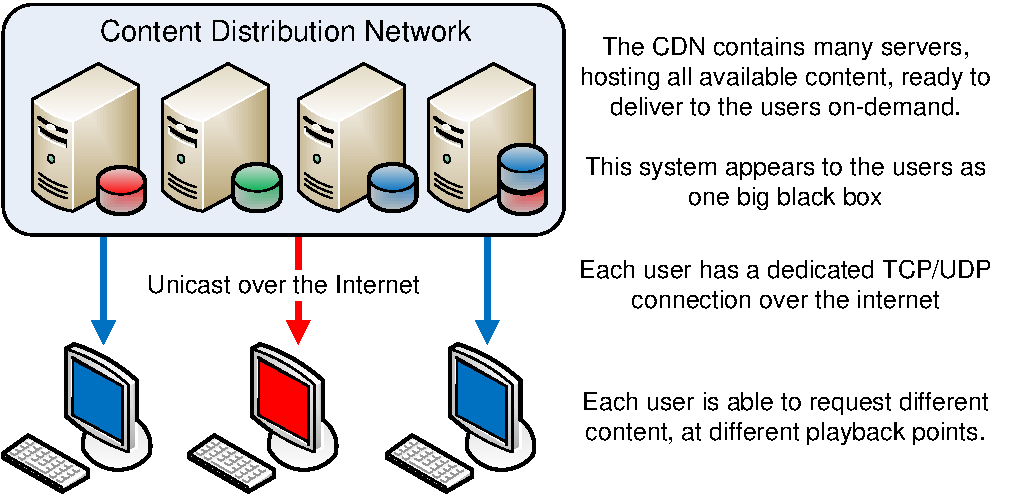
\includegraphics[width=0.7\columnwidth]{./diagrams/CDN}

    \caption
        [Distribution of media via a content distribution network]
        {Distribution of media via a content distribution network. Different coloured arrows and shapes represent the different content.}
    \label{fig:cdn}
\end{figure}

    The HTTP servers used for streaming are typically hosted by a content distribution network (CDN) as depicted in \autoref{fig:cdn}. Little is known about how these systems are configured and deployed, however some research has gone into inferring their deployment by taking measurements. In one study, Saxena~\emph{et~al.} found that YouTube's videos are served from just two main locations in the US; San Mateo (77\%) and Mountain View (22\%), with the remaining 1\% being served by the Limelight's CDN~\cite{saxena2008avs}. This suggests most of YouTube's CDN is built and controlled in-house. Saxena~\emph{et~al.} also found that Metacafe took a different approach and outsourced their needs to the Akamai and L3 Networks CDNs. It is well know that Akamai position their servers into as many ISP's points of presence (POPs) as possible~\cite{huang2008uhc}.

    Until very recently these UGC sites had limited interactive controls. The Flash player would continue to buffer the video being viewed as fast as possible and store everything which has been received in a temporary file on the computer's hard disk. Users were able to pause, and seek backwards into the stored buffer, but were unable to seek ahead of the buffer. Since late 2007/early 2008, YouTube and others have begun allowing arbitrary seeks anywhere in the media before it is buffered. This has been achieved using a custom client-side Flash player and some server software. How exactly this is achieved is discussed later in \autoref{sect:seekable_flash}, as this technique was developed independently by us before it had been implemented by YouTube.

\subsection{BBC iPlayer}
\label{sect:bbciplayer}
% Nic has read
%TODO Last sentence mentions network PVRs before they are discussed!

    BBC iPlayer~\cite{iplayer} has been leading the way as a new type of desktop application which enables users to watch video-on-demand over the internet, using a normal home broadband connection. BSkyB and Channel~4 have also created similar products to compete with the BBC, named Sky Player~\cite{skyplayer} and 4oD~\cite{4od} respectively. These products differ from network PVRs, as they serve a more specific task, and do not require custom hardware.

    These products offer a catalogue of old programmes (which are no longer regularly shown on broadcast TV), and access to most of the broadcast programming shown in the last 7~days. Users can select which programme they want, and their client begins to download the video. However, these products do not stream the video; instead they download a single file. This means the user must wait until the full file is downloaded before playback can start.

    All three applications are actually based on one companies technology, Kontiki~\cite{Kontiki}. This company has created their own technology to provide a content delivery platform, which can securely deliver media from standard servers, assisted by scalable peer-to-peer techniques. Kontiki is closed source software, and as far as we are aware no studies have been conducted to analyse how it works. However, from promotional material, it constructs a simple peer-to-peer network from the users. This network can be configured to limit how the peers are connected, for example, making sure the peers do not connect outside of their own subnet, or autonomous system (AS) boundary.

    When a Kontiki client is idle, any spare bandwidth is used to help spread the content within the network. To seed the content into the peer-to-peer network, and to provide additional capacity, a normal network of servers deployed in a CDN are used. This peer-to-peer network does not allow users to publish their own content, as the network is used just as the provider's content delivery platform. To ensure this requirement is met, the network uses strong cryptographic techniques such as asymmetric cryptography~\cite{rivest1978mfo}, to guarantee that media is not tampered with, and also to ensure that new media is not injected into the network without permission.

    The files published by the BBC are typically Windows Media (WMV) files, protected with digital rights management (DRM). The DRM stops the files from being shared with others, and expires the files a few days after playback. These files are of good quality, and are roughly 140~MB for a 30~minute show. Since the full WMV files are downloaded before playback can begin, interactive controls are easy to provide. Pausing and seeking to arbitrary points is readily available, and instantaneous.

    Due to the Kontiki platform, and the DRM techniques, the iPlayer software only runs on Microsoft Windows, and not on other operating systems such as Linux, or Apple's Mac OS. This received many criticisms, as the publicly funded BBC were ignoring a subset of the public that did not use Windows. To counter, this the BBC introduced a new streaming based iPlayer which could be accessed via their website. This uses Adobe Flash technology, similar to that used by many user generated content sites, such as YouTube. By creating their Flash based site, any device which could render Flash video was now able to view the iPlayer's catalogue. This includes desktop computers running various free operating systems, many home gaming consoles, such as the Nintendo Wii~\cite{bbc2008ban} and Sony Playstation 3~\cite{purchese2008fmb}, and mobile devices such as the Apple iPhone~\cite{bbc2008bic}.

%    \todo{Briefly recap what interactive features are available with the online iPlayer}

\subsection{Personal Video Recorders}
\label{sect:pvr}

% Nic has read

\begin{figure}[t]
    \centering

    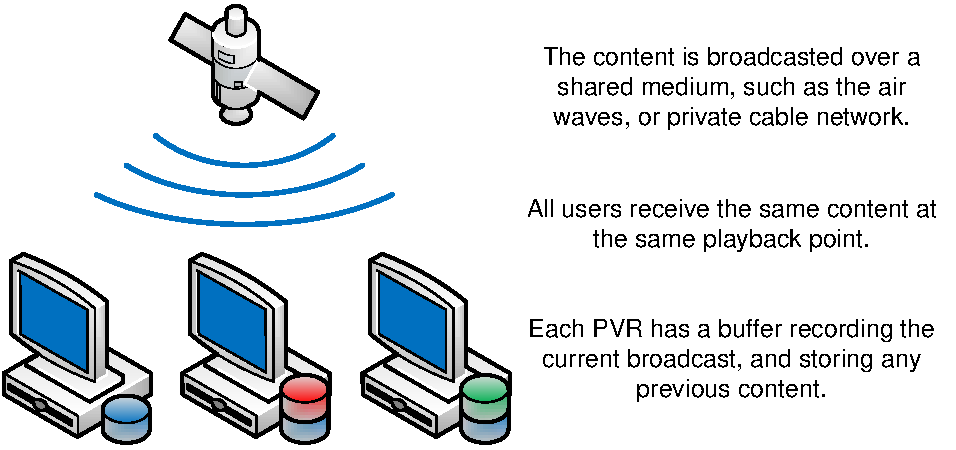
\includegraphics[width=0.7\columnwidth]{./diagrams/PVR}

    \caption
        [Distribution of media in a boardcast personal video recorder network]
        {Distribution of media in a boardcast personal video recorder network. Different coloured arrows and shapes represent the different content.}
    \label{fig:pvr}
\end{figure}

    %"More than half (57\%) of all UK residents �time-shift� their TV viewing, using on-demand TV services or recording live television for viewing later", "36\% use a PVR"~\cite{YouGov2008red}

    A device that is becoming more commonplace in the living room, is the \emph{time-shifting} set-top box. These devices, sometimes called personal video recorder (PVR) or digital video recorder (DVR), are typically set-top boxes which record broadcast TV. These PVRs allow the user to pause playback while the box continues to record, or rewind within the recording. Additionally, if the user has paused or rewound, they may fast forward to catch up with the live broadcast. It was estimated in 2008 that 36\% of the UK uses a PVR~\cite{YouGov2008red}.

    There are many PVRs on the market, the most popular being, Sky+~\cite{sky+}, TiVo~\cite{tivo}, ReplayTV~\cite{replaytv} and UltimateTV~\cite{ultimatetv}. The Sky+ PVR, for example, records broadcast TV received via a satellite dish as seen in \autoref{fig:pvr}. This PVR has two TV tuners, allowing it to record from two channels simultaneously. As with most of these devices, it contains a large hard disk, able to record within the range of 40 to 80~hours of TV.

    The Sky+ box can be scheduled to record future TV programmes or films via the electronic programme guide (EPG). Once recorded, the user is able to play the recorded programmes by selecting them from the EPG. However, this does not give the user a true video-on-demand experience, as they have to wait until the programme airs before being able to watch it. To combat this, Sky+ has recently integrated a \emph{push video-on-demand} system called ``Sky Anytime''. Sky can instruct the Sky+ box to record popular programming, such as new movies, or sporting events. The programming is sent on hidden broadcast channels, typically during the night when the Sky+ box is not in use. Users can then chose any of these ``Anytime'' programmes, and play them back instantly from their local hard disks.

    The interactive controls are rather limited with these boxes, as they are only able to seek within what is currently buffered. In live TV that means rewinding, but in pre-recorded content (such as ``Sky Anytime'') they may fast-forward or rewind. To allow rewinding with live TV, the Sky+ box is always recording the current channel, with a buffer of up to two hours. Once the channel changes, this buffer is discarded and a new one begins. This allows a user to pause for no longer than two hours, and rewind the current channel up to a maximum of two hours (as long as the channel is not changed within that time).

    %TODO cite staggered broadcast
    Most satellite providers also offer pay-per-view content, such as very new movies, or live one-off sporting events. Events, such as sports, are typically broadcast live on a single encrypted channel, which limits the interactivity to simple pause and rewind. More interesting are the \emph{near video-on-demand} services. These are typically provided for movies, where a single movie will be broadcast on multiple channels using a simple staggered broadcast technique. If staggered, the movie will be broadcasted at fixed time intervals, for example, every 15 minutes. Thus, when a user purchases a movie they will have to wait up to 15 minutes to begin watching.

    Near video-on-demand has the ability to allow users to seek forward or backwards in fixed time intervals, for example, 15 minutes at a time. When combined with a PVR, this can be extended to allow more fine grained seeking, if for example, the PVR records two broadcast channels at different positions within one programme. This could allow the PVR to buffer 15 minutes ahead, by using the second channel. Once the first channel has caught up to the buffer, it can begin playback from the buffer, and use the first channel to record 30 minutes ahead. This process can continue until the full movie is buffered to disk. As far as we are aware, no set-top box offers such functionality, mostly due to the added complexity for little gain.

\subsection{Networked Set-top Boxes (IPTV)}
%Nic has read

    %TODO \cite{olausson2007gif} predicts there will be 80 million IPTV users by 2011

    Some set-top boxes, those typically on cable networks, have begun to roll out IPTV services which offer true video-on-demand. In the UK, the main provider is Virgin Media with over 3 million customers using its ``On Demand'' service~\cite{virgin2008on}. British Telecom (BT) have also recently introduced a similar product called ``BT Vision''~\cite{bt2008bv}. It is predicted that by 2011, there will be 80~million IPTV users worldwide~\cite{olausson2007gif}.

    In these systems, a simple set-top box or PVR is connected to either a private network (in the case of Virgin Media), or via the public internet. Content is then streamed directly to the user instantly, on-demand. Virgin Media have been able to offer this service for many years by utilising the existing cable network infrastructure to unicast video from the user's local head-end\footnote{A head-end is a facility run by a cable company to serve customers in the local region}  directly to the end-user. This is not possible in satellite or traditional radio broadcast as both have finite broadcast capacity, whereas cable networks have constantly invested in and improved their networks over the years, adding more and more capacity.

    Nevertheless, the on-demand content which is available via these services seems to be of lower than normal broadcast quality, and little is known about the technical details. However, from experiments with these set-top boxes it may be possible to infer how they operate. For example, examining Virgin Media's On Demand service, it is clear that a staggered broadcast system is being used. When seeking through the video, the video jumps in increments of 15 seconds, and when starting a new video it takes up to 15~seconds to begin. This may be because the video is being broadcast in staggered intervals of 15~seconds. It is unclear if this is done so a broadcast technique such as multicast may be used, or if this is to reduce the number of unique channels the server has to transmit.

    One feature which Virgin Media does offer, that no other streaming VoD service provides, is the ability to fast-forward or rewind (\emph{e.g.} to view the video at a faster rate either forwards or in reverse). Again, however, this service is limited to just a couple of fast-forward or rewind speeds. Also, when starting or finishing to fast-forward or rewind, the video appears to jump or stutter. This may be because there are dedicated streams broadcasting the video at a higher speed forwards and backwards. Thus, when the set-top box is instructed to fast-forward, it actually joins this different faster stream.

    The system being offered by BT is powered by software created by Microsoft named Mediaroom~\cite{microsoft2008m}. This software is also being used by numerous IPTV providers around the world, such as, T-Home (German), Portugal Telecom (Portugal) and AT\&T (United States). Most of these providers are using cable or fibre to deliver broadcast quality content to the homes. However, BT have taken a different approach, and are using traditional home ADSL broadband technology. We speculate that this is because of the higher ADSL penetration in the UK, and that cable/fibre networks in the UK are almost exclusively owned and operated by Virgin Media.


\subsection{Peer-to-Peer}
\label{sect:peer-to-peer}

\begin{figure}[t]
    \centering

    \subfloat[][Tree P2P Network] {
        \label{fig:p2p-tree}
        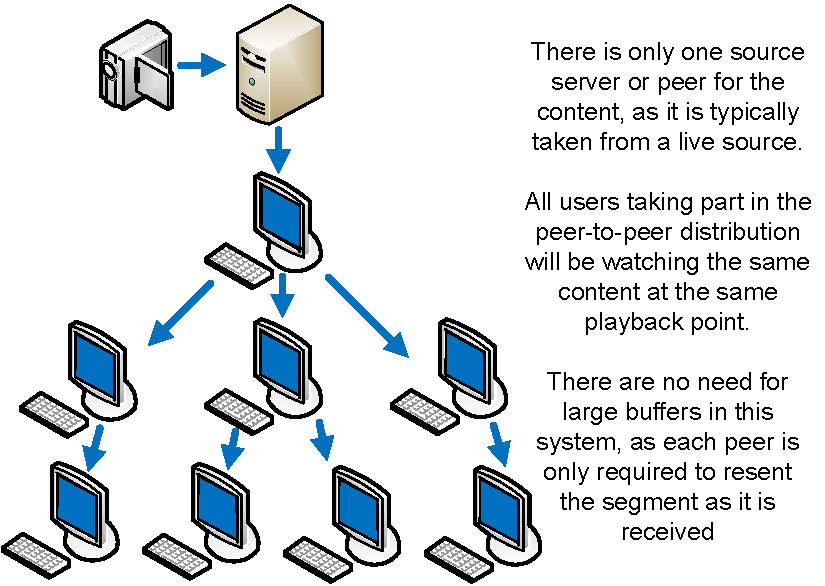
\includegraphics[height=5cm]{./diagrams/P2P-tree}
    }
    \subfloat[][Mesh P2P Network] {
        \label{fig:p2p-mesh}
        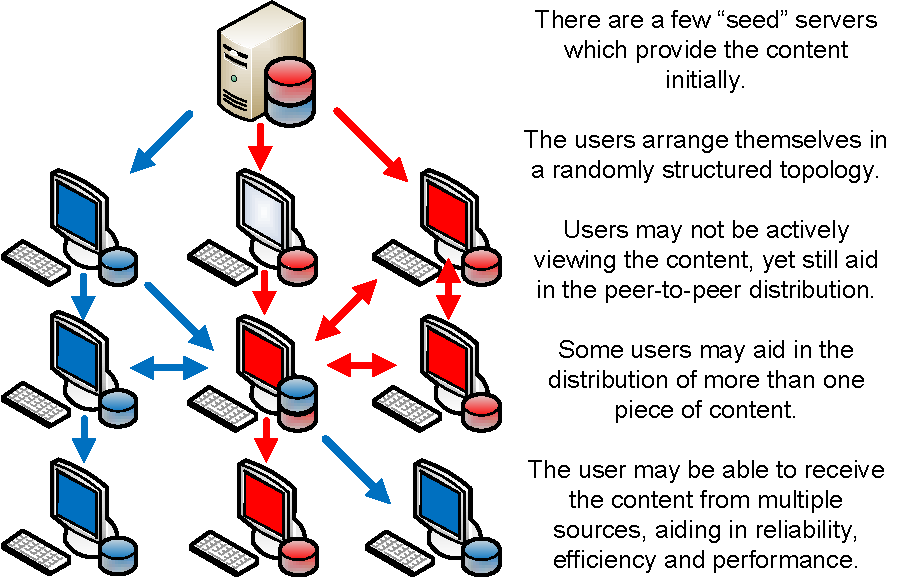
\includegraphics[height=5cm]{./diagrams/P2P-mesh}
    }

    \caption
        [Distribution of media in a peer-to-peer network]
        {Distribution of media in a peer-to-peer network. Different coloured arrows and shapes represent the different content.}
    \label{fig:p2p}
\end{figure}

    Other than the previously mentioned commercial online video-on-demand systems, there are numerous peer-to-peer (P2P) technologies that enable efficient streaming of live and stored media~\cite{liu2008spp,li2007ess}. Traditional P2P has been used to distribute full files~\cite{cohen03ibr,emule,gnutella}, including files such as movies, tv shows, music~\cite{napster}, \emph{etc}. As the full file must be downloaded before playback can begin, this can be considered a primitive form of VoD, similar to that offered by the Kontiki based applications (see \autoref{sect:bbciplayer}).

    After the initial surge of P2P file sharing applications, research began on application level multicast (ALM)~\cite{yeo2004sal}, sometimes called end-system multicast~\cite{chu2002ces}.  This is a form of P2P designed to stream content, in a one-to-many fashion, similar to traditional IP multicast. However, streaming is different to video-on-demand, as all the users are typically viewing the same content at the same playback point.  Video-on-demand should allow users to view different content at different playback points simultaneously, which makes it much more problematic.

    Only recently has research began into the areas of peer-to-peer video-on-demand (P2P-VoD). Using P2P offers many advantages over the traditional client-server approach. Firstly, peer-to-peer can greatly reduce the costs to run the service, as a large CDN is not required to deliver the content. Additionally, in the mesh-based P2P, those able to request from multiple sources simultaneously have advantages when it comes to interacting with the media. These protocols are designed to allow arbitrary segments to be downloaded. Thus, seeking and pausing can occur relatively easily.

    Peer-to-peer does have some disadvantages, such as additional overheads and requiring peers to take part in the delivery. These overheads are from the extra control traffic needed to arrange peers into a structure suitable for media delivery. As peers are the main source of content, they can be less reliable and have less resources than tradition servers. This may result in unpredictable or unreasonable service. Additionally, unless a content protection scheme is used, peers may maliciously alter the content when relaying to other users~\cite{dhungel2007pap}. Also, not all peers have sufficient capacity or want to take part in the network.

    When describing P2P, there are a few different ways the networks may be arranged and how the data is transmitted.
\begin{description}
  \item[Tree] In tree distribution, the peers arrange themselves in a tree, rooted at the source of the content (as depicted in \autoref{fig:p2p-tree}). This is best used for streaming, as there is typically only one source for this kind of content. The content can then be streamed down the tree, and eventually reach every peer. There are many protocols which efficiently arrange peers in this manner~\cite{mathy01otb,banerjee2002sal,tran2003zae}. However, it was noted~\cite{castro2003shb}, if nodes are arranged in a tree, the leaf nodes (those at the bottom) do not distribute to others. This is an obvious waste of resources, as $f^h$ peers within the network do not help distribute the content, where $f$ is the node's out-degree and $h$ is the height of the tree. To better utilise the resource, multi-source trees were developed~\cite{begen2003mps,castro2003shb}. These multi-source trees also make the distribution more robust to failures, such as, a node parent failing~\cite{do2004ppf}. One problem for all trees, is that they may become very deep, causing a high latency (or lag) for the peers near the bottom.

  \item[Mesh] To improve the efficiency of tree based schemes, mesh networks create a seemingly randomly connected graph from the peers~\cite{kostic2003bhb,liao2006app,magharei2007ppp,hei2008iop}, as seen in \autoref{fig:p2p-mesh}. Content may then flow in any direction through this graph, allowing each peer to have many sources, as well as many nodes to share with. This technique is typically used to provide video-on-demand~\cite{annapureddy2006pvd} or file distribution~\cite{cohen03ibr}, as it offers greater reliability and performance, at the cost of additional overheads and less guarantees of the ordering of received data. Unfortunately, peers within a mesh network will experience a higher rate of churn (peers joining and leaving), as each peer is potentially connected to tens of others.
\end{description}

Typically the content is always divided into segments, of fixed (or sometimes variable) size. This allows peers to request individual chunks of the media, as well as to more efficiently inform others which segments they has. The segments are normally either pushed or pulled by the peers though the peer-to-peer network.

\begin{description}
  \item[Push] Push distribution is typically used for live streaming in combination with tree based distribution. In live streaming each peer will require the segments by a similar deadline, and each peer typically only has one parent, the segments can be pushed to the peer, without request. This greatly reduces the overheads of knowing which peer needs which segment, \emph{etc}. Push can also be used in multi-source situations by clever partition tricks, for example, in a two-source situation, a peer can receive odd segments from one peer, and even from the other. However, this gets increasingly complex when there are multiple source peers or the network is in a constant state of churn (as is common in mesh networks).

  \item[Pull] If it is not obvious which peer needs which segment, then pull distribution is better. Each segment must be explicitly requested by the peer before it is sent. This adds additional overheads, but allows the receiving peer to make decisions on where to receive from. Pull is popular in mesh networks, as it simplifies the distribution of content. To allow pull to work, each peer must occasionally share a list of currently buffered segments with their neighbours. This list is typically shared in the form of a bit-map, assigning a one or zero to each segment, indicating whether it is buffered or not.

\end{description}

    This rest of this section discusses the main peer-to-peer systems in both the streaming, and VoD domains.

\subsubsection{Streaming}

    Streaming, is typically used for live events, or broadcasting of traditional style television channels. As such all the users will be viewing the content at the same playback point, as opposed to video-on-demand, which allows users to view different playback points simultaneously.

    There are many commercial peer-to-peer streaming products available, mostly from Chinese companies. These include PPLive~\cite{pplive}, CoolStreaming~\cite{zhang2005cdd}, Zattoo~\cite{zattoo}, TVAnts~\cite{tvants}, PPStream~\cite{ppstream} and SOPCast~\cite{sopcast}. This software has been very popular in China~\cite{fowler2005nef}, and is starting to become more popular in the US/UK.

    CoolStreaming (or more formally known as DONet) was one of the most popular services, when it was in operation. Information about how the system works was made publicly available, and a couple of papers were published on the topic~\cite{zhang2005cdd,xie2007cdt}. However, in 2005 the service stopped broadcasting, less than a year after it first began, due to copyright issues.
% TODO I need a reference for the copyright issue, but I couldn't find one :(

    The CoolStreaming technology is based on a pull mesh-based streaming technique. When joining the system, a newly connecting peer would obtain a list of existing peers from a central repository.  This list would be used to bootstrap the newly connecting peer into the network. Afterwards, a gossip protocol is used to find additional peers. Segments of the media are there pulled from neighbouring peers, who frequently advertise their segment lists.

%   The stream is divided into equally sized segments.  Each peer maintains a local buffer of segments. A list of the peer's segments is occasionally shared in the form of a bit-map, with directly connected peers. Sharing the list allows other peers to know which segments of the stream the peer has. Then, in a pull fashion, a peer can request segments required for its own playback.

    One of the novel features of CoolStreaming is the scheduling algorithm which decides which peer is used for a segment when there are multiple peers to chose from. The problem of deciding the most efficient way for each peer to allocate it's resources is an NP-hard problem, akin to parallel machine scheduling~\cite{cormen2001ita}. Therefore, CoolStreaming uses a simple heuristic to decide the allocation of resources. The algorithm uses a combination of how rare the segment is, how much free bandwidth the remote peer has, and how urgently the segment is needed.

    PPLive~\cite{pplive} is more popular than CoolStreaming, as it has a total of 2.2 million users and 500 different streams~\cite{huang2008cda}. A keynote presentation by Huang, a PPLive Software Architect, demonstrated how scalable P2P streaming can be. In the second quarter of 2007, PPLive supported 1,480,000 simultaneous users viewing the same live sporting event, being served by just one 10Mbit/s server~\cite{huang2007ewp}.

    Even though PPLive is a closed-system it has been a hot-topic for researchers to study~\cite{huang2008cda,silverston2007mpi,vu2007mls,krieger2008aaq,chen2008msc}. Silverston and Fourmaux captured traces from PPLive, and determined it uses a mesh-based pull approach, similar to CoolStreaming~\cite{silverston2007mpi}. Vu~\emph{et~al.} noted that PPLive tries to keep its neighbour peer list around 30 to 45, independent of the number of peers currently taking part in the stream. By keeping the neighbour list around a constant size, this allows the system to scale far more efficiently~\cite{vu2007mls}.

    Vu~\emph{et~al.} also calculated the \emph{clustering coefficient}~\cite{watts1998cds} of this network. This is a measure of how randomly the peers are connected to each other. They found streams with few peers ($<500$ peers) had a high degree of randomness, however, as the stream size increased, many clusters of peers began to form. They did not speculated as to whether the clusters were based on some metric of ``closeness'', \emph{i.e.} network or geographical locality.

    The remaining studies which look at PPLive have looked at simple metrics such as packet size~\cite{krieger2008aaq}, signal overhead~\cite{silverston2007mpi}, stream popularity, and chunk availability~\cite{huang2008cda}. These do not give much insight into how PPLive operates. However, one thing is clear, PPLive is a large peer-to-peer application which has tremendous scaling abilities. This is only let down by the fact that it is a pure streaming application, and does not offer interactivity features beyond pause and resume. Nevertheless, PPLive will encourage development of future projects which take advantage of this form of streaming peer-to-peer, hopefully with addition VoD features.

%Nic has read to here

    % [2] �PPLive�, http://www.pplive.com/.
    % PPLive ( Challenges, Design and Analysis of a Large-scale P2P-VoD System )
    % As of late November 2007, a total of 2.2 million independent users had tried the system. A total of 3900 movies were published in November and December of 2007, with around 500 movies on-line simultaneously. In late January 2008, the number of simultaneous users reached over 150K and was still growing

\subsubsection{Video-on-demand}

    Peer-to-peer video-on-demand (P2P-VoD) typically uses a combinations of P2P file sharing and streaming techniques. Users will contribute local disk space, as well as bandwidth, to allow other users to stream directly from them. Typically the local disks will store multiple videos which have been previously watched, and perhaps a few which have not if the network deemed their replication necessary. Many of the pure streaming techniques can be applied, or slightly altered, to work for video-on-demand. However, this is easiest with the pull based systems, which can easily cope with peers being at different playback points.

    There are a number of commercial systems, such as, Vuze~\cite{vuze}, Joost~\cite{joost} and many others~\cite{gridcast,pfsvod,ppstream,uusee}. Again, all of these systems use proprietary techniques, and as such the only information about them is inferred, or discovered through measurements.

    Vuze, for example, offers a catalogue of thousands of videos, mostly uploaded by users, but some from professional studios. To download the videos Vuze uses a sliding window BitTorrent~\cite{cohen03ibr} technique~\cite{vlavianos2006beb,shah2007ppm}. To begin viewing a video, Vuze must connect to a tracker. The tracker is a centralised server or possibly decentralised in some modern BitTorrent implementation~\cite{roozenburg2006sds}. The tracker maintains a list of all peers who are in the process of downloading, or have finished and now just sharing. The Vuze client uses this list to form a single P2P network for each video.

    Normally, BitTorrent connects to as many peers in the P2P network as possible and begins downloading. Multiple downloads occur in parallel, each requesting a different random segment of the full file\footnote{BitTorrent does not always download segments in a random order, as there are multiple improvements to increase the efficiency of the ordering~\cite{massoulie2005crs}}. The random order helps ensure that the file is spread as quickly as possible throughout the network~\cite{bharambe2005aai}. So that Vuze can display the video to the user as it downloads, it opts to download the segments of the file in a semi-sequential order. A sliding window is created ahead of the playback point, and only segments within this window are downloaded. As playback continues, the window moves along.

    In theory, Vuze could support many interactive controls, however, it only supports pause and resume. Pause is a simple operation as playback from the buffer can stop while not affecting the normal download. Seeking is not possible as time offsets cannot be easily mapped to file segments.  This feature could be added if metadata provided a map of keyframe times to an offset within the file. Then on a seek request the sliding window can be moved to the new seek location, and download/playback resume.

    There are numerous problems with Vuze, for example, the protocol is a very simple modification to BitTorrent, which is not custom-made for this task. This causes the start-up times to be long, and limits the interactive features. Also, because the peer-to-peer networks are only made up of peers who have previously downloaded, or are downloading, the video, it is possible for the video to not be fully available. A more suitable situation would be to either backup the videos on dedicated content servers, or ensure the videos are replicated on nodes with spare capacity, therefore better utilising the network.

    Joost~\cite{joost}, takes a different approach to Vuze, by designing a new P2P-VoD protocol from the ground up. Joost, was created by Niklas Zennstr\"om and Janus Friis, the two entrepreneurs responsible for Skype~\cite{skype} and Kazaa~\cite{kazaa}. Joost has a large catalogue of content, which is provided exclusively by professional studios. Because of Skype's and Kazaa's fame, Joost has been able to secure deals with many large studios, such as FOX networks, Viacom (which includes MTV and Paramount Pictures), and Warner Music. This has allowed Joost to have high quality content, such as feature films and TV episodes.

    Little is know about Joost, however it is reported that it is a mesh based peer-to-peer network backed by servers deployed in a CDN. From one study, it appears that Joost uses UDP packets, to transmit content in MPEG-4/AVC with error-resilience coding~\cite{krieger2008aaq}. It is speculated that Joost will use peers with spare capacity to help distribute content which is popular. This would help to maximise the delivery efficiency.


\subsection{Summary}

% TODO write about this figure!
%\begin{figure}[t]
%    \centering
%    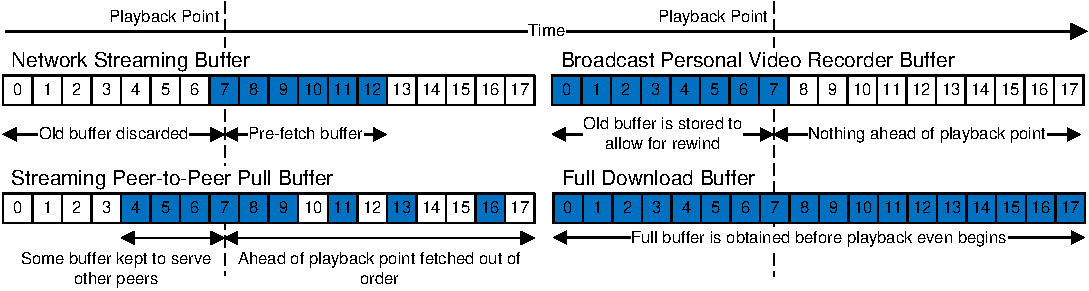
\includegraphics[width=1\columnwidth]{./diagrams/buffers}
%    \caption{Layout of buffers used by various systems}
%    \label{fig:buffers}
%\end{figure}

%\begin{table}[t]
%    \centering
%    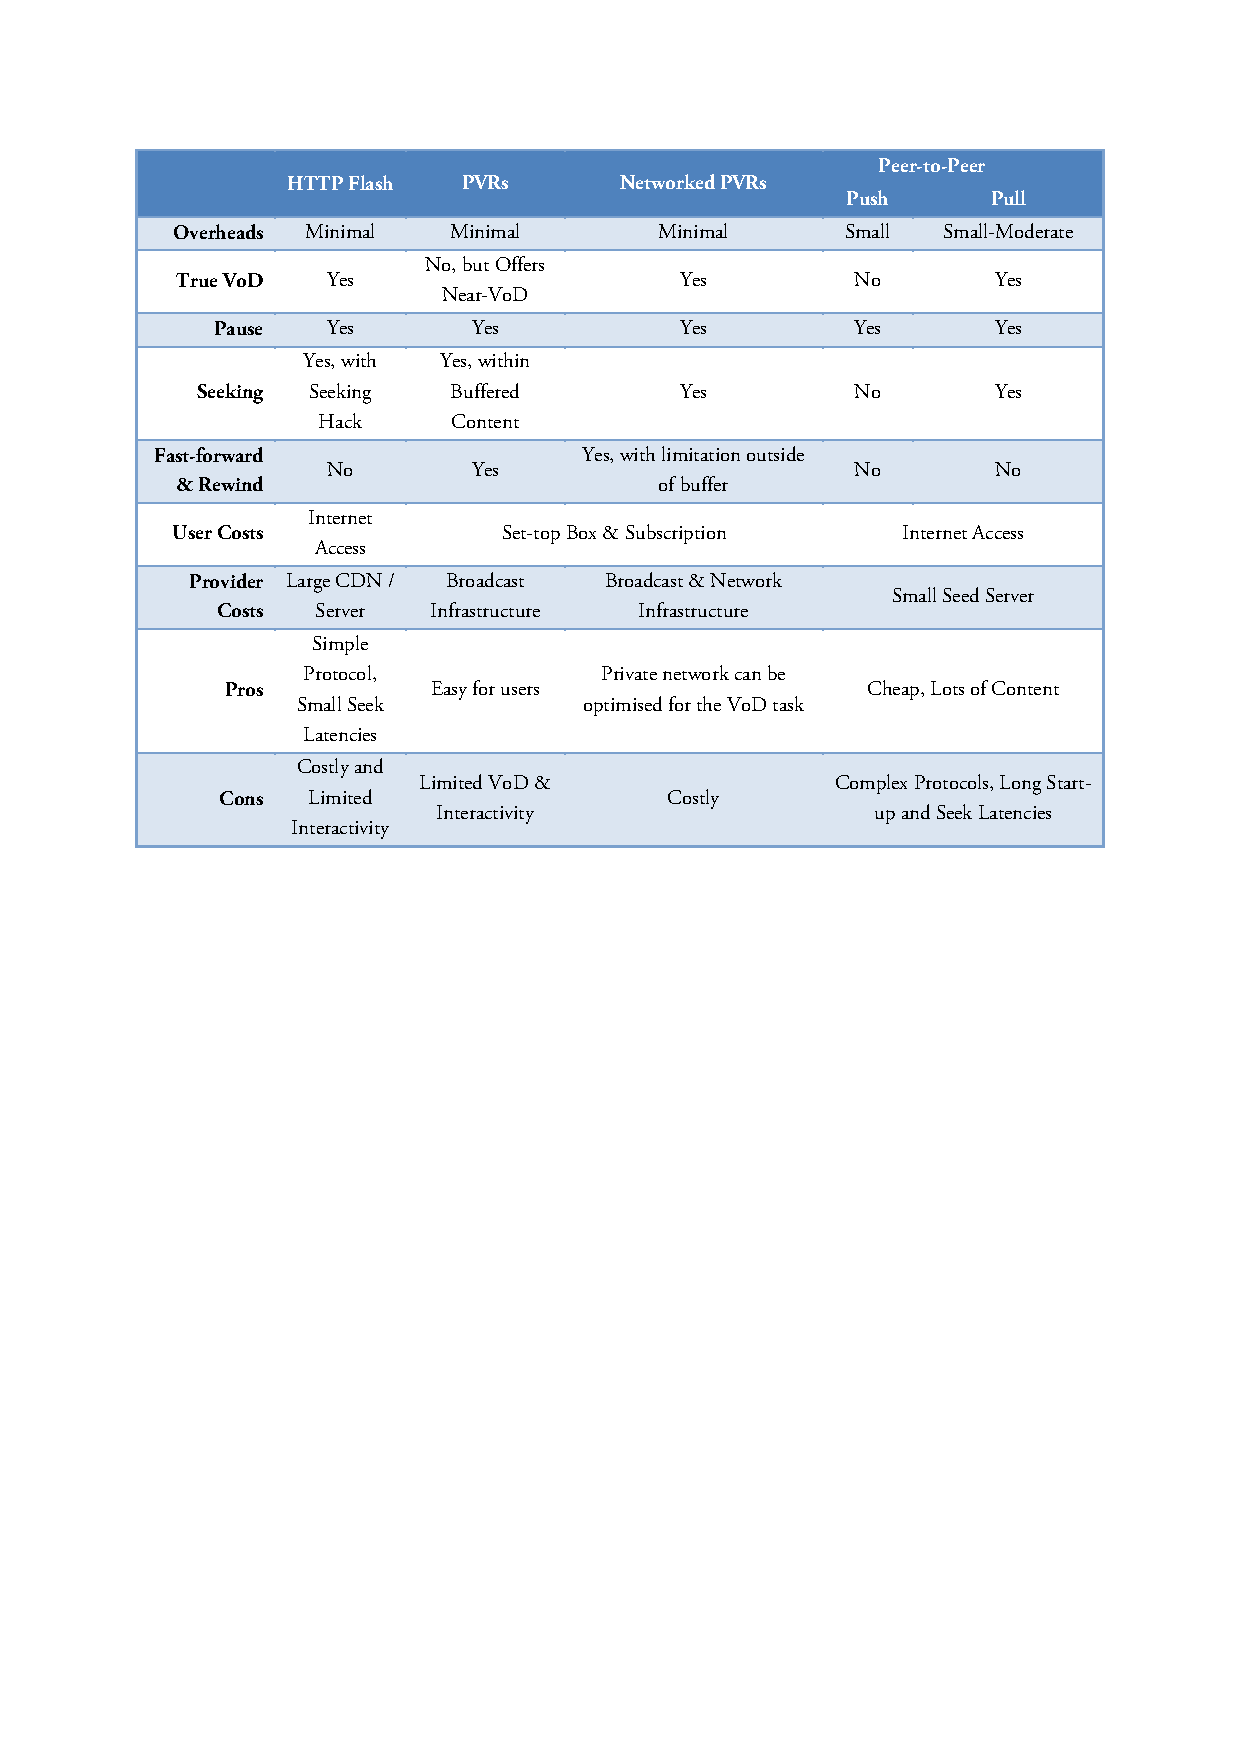
\includegraphics[width=1\columnwidth]{./diagrams/table}
%    \caption{Summary of features available with each video-on-demand system}
%    \label{fig:vod_table}
%\end{table}

\begin{table}[t]
\setlength{\tablecolwidth}{0.14\columnwidth}
\newcolumntype{C}{>{\centering\arraybackslash} m{\tablecolwidth} }
\newcolumntype{R}{>{\raggedleft\bfseries\arraybackslash} m{\tablecolwidth} }
\scriptsize
    \begin{tabular}{|RCCCCC|}
\hline
\setrowcolor{TableRowHead}
                    &  &  & & \cellendbxy{2}{1}{Peer-to-Peer} \\
\setrowcolor{TableRowHead}
                           & \cellbxy{1}{-2}{HTTP Flash} & \cellbxy{1}{-2}{PVR} & \cellbxy{1}{-2}{Networked PVR} & \textbf{Push}   &\textbf{Pull} \\
\hline
\setrowcolor{TableRowA}
    Overheads              & Minimal & Minimal & Minimal &  Small  & Small-Moderate\\
\setrowcolor{TableRowB}
    True VoD               & Yes & No, but offers Near-VoD & Yes & No & Yes\\
\setrowcolor{TableRowA}
    Pause                  & Yes & Yes & Yes & Yes & Yes \\
\setrowcolor{TableRowB}
    Seeking                & Yes, with Seeking Hack & Yes, within Buffered Content & Yes & No & Yes\\
\setrowcolor{TableRowA}
    Fast-forward \& Rewind & No & Yes & Yes, with limitation outside of buffer & No & No \\
\setrowcolor{TableRowB}
    User Costs            & Internet Access & \cellxy{2}{1}{Set-top Box \& Subscription} & \cellendxy{2}{1}{Internet Access} \\
\setrowcolor{TableRowA}
    Provider Costs         & Large CDN / Server & Broadcast Infrastructure & Broadcast \& Network Infrastructure &  \cellendxy{2}{1}{Small Seed Server} \\
\setrowcolor{TableRowB}
    Quality                & Low--Medium & High & High & Medium & Medium \\
\setrowcolor{TableRowA}
    Pros                   & Simple Protocol, Small Seek Latencies & Easy for users & Private network can be optimised for the VoD task  & \cellendxy{2}{1}{Cheap, Lots of Content} \\
\setrowcolor{TableRowB}
    Cons                   & Costly and Limited Interactivity  & Limited VoD \& Interactivity & Costly & \cellendxy{2}{1}{Complex Protocols, Long Start-up and Seek Latencies} \\
\hline
    \end{tabular}
    \caption{Summary of features available with each video-on-demand system}
    \label{fig:vod_table}
\end{table}

%    \todo{Summarise this whole section}
%    \todo{Outline the pros and cons for each concept}
%    \todo{Where do innovation need to come?}

%\begin{itemize}
%  \item Content Distribution
%      \begin{itemize}
%        \item high cost
%        \item low overhead, potentially best service for users
%        \item Can offer interactivity, but extra load on servers
%        \item Simple
%      \end{itemize}
%
%  \item PVRs / Network PVRs
%      \begin{itemize}
%        \item Most integrated, simple for users
%        \item Most be deployed, at cost to the users
%        \item No interactivity unless networked
%        \item Networked has similar problems to CDNs
%      \end{itemize}
%
%  \item Peer-to-Peer
%      \begin{itemize}
%        \item low cost
%        \item high overhead
%        \item Push has lower overheads than pull, but makes it harder to do VoD.
%        \item Users don't want to pay for a server, and upload
%        \item Additional problems, ie stop tampering, seeding own content.
%        \item The pull mechanisms do aid in interactive features
%      \end{itemize}
%\end{itemize}


    The previous sections have outlined popular video-on-demand systems which are currently deployed and in use. Their features have been explained, as well as the pros and cons of using them. Here, we will summarise the previous sections, and aim to discuss the systems compared to each other. To recap, \autoref{fig:vod_table} lists the main categories of systems, and which features they support.

    The HTTP Flash-based systems are typically backed by a content distribution network (CDN), but can in small cases be simple client-server systems. By using a simple \emph{pseudo-streaming} technique, the flash-based web-site is able to provide videos on-demand to a vast audience of users via the internet with minimal overheads and costs to the user. However, the back-end system, will no doubt involve terabytes of replicated data, spread across hundreds if not thousands of servers, typically deployed throughout the world. The cost of running such an infrastructure is not cheap, for example, in 2006 it was estimated that YouTube pays \$1~million a month just for bandwidth costs~\cite{frommer2006ytw}. As such, only the well funded content providers can afford to provide this service.

    Content distribution networks used by Flash-based systems can provide many of the modern interactivity features requested by users, albeit with additional overheads and complications for the servers. The one downside when interacting with these systems is the seek-delay. This is normally quite small (less than 2~seconds), and no longer than a couple of round trip delays, and the time it takes to fetch an initial buffer. This can be reduced by making sure the content servers are near to the end users.

    Personal video recorders (PVRs) are perhaps the simplest system for users, as they integrate with users' existing home entertainment systems. If the content provider is already broadcasting the content, then the cost for deploying the PVRs is just the price of the box. However, a simple broadcast-only PVR does not allow for true VoD, only being able to watch pre-recorded content. To add true VoD, dedicated networks are typically used, which greatly increase the cost for the provider. Regardless, PVRs are able to record content at broadcast quality, which is much higher than that typically found on the internet.

    Finally, the peer-to-peer model of distribution offers the cheapest way to deliver content, and if it is not streamed (and instead downloaded) the highest quality of content. This allows independent movie studios, or amateurs to easily release their work in high-def quality formats. Being cheap comes at the cost of requiring users to aid in the distribution, which typically involves high signalling overheads, for example, to coordinate all the peers in a distributed manner. Aiding in distribution is unappealing to many, as they either have to pay for their bandwidth, or are unwilling to share their resources if they are required to pay for the content or service.

    Peer-to-peer also offers numerous other challenges, which can vastly affect the performance of the system. Unlike with CDNs and PVRs, the relative simplicity of the protocols allows them to have a high level of service and reliability. However, in peer-to-peer, your level of service depends on other users, who join and leave the network as they choose. Also, if a user decides to be malicious, they may disrupt the network, inject illegal content, or tamper with the existing content.

    The added complexity of P2P does allow for higher levels of interactivity. For example, in pull based P2P, the content may be fetched out of order.  It is therefore trivial for the protocol to fetch new seek points, or to even pre-fetch ahead to areas of interest. Features like this reduce seek delay, but this improvement may be negated because of the high overheads and unreliable performance of other peers. There is certainly room for much improvement and innovation to solve the numerous challenges found within P2P.

%\todo{Some how get my story across}

%\subsection{Motivation}
%%    \item Discussion on Interactivity and how it breaks streaming
%%    \begin{itemize}
%%        \item Introduction
%%        \item Push/Pull Techniques~\footnote{incorporating Andy's Hybrid work.}\saveFN\andy\
%%        \item Hybrid concepts~\useFN\andy\
%%    \end{itemize}
%
%    "Exploring prefetching to improve the scalability of these protocols for interactive workloads is left for future work."~\cite{costa2004aci}


\section{Characterisations of User Behaviour}
\label{sect:characterisations}

%todo add some diagrams to explain the models

%\todo{Add a interactivity spin, to make it clear we need to understand interactions}

%"can help in designing and evaluating call admission strategies [3], scalable compression techniques [18], and client/server buffer management strategies [4] for CM systems"~\cite{padhye1999cmc}

To design systems that support the delivery of multimedia over the internet, it is crucial to understand how users will interact with the media. These interactions impact multiple functions, such as, admission strategies, buffer management and delivery techniques.

In a content distribution networks (CDNs) context, this could effect how proxy servers operate, and how the location of replicated media, and which delivery mechanisms are used. If, for example, only a small subset of media from a large catalogue is popular then more resources should be dedicated to those popular files. Content could also replicate in advance, if it was possible to anticipate demand. This is all possible by understanding how the content is consumed by the user.

One area which has not been closely examined, is when there are high levels of interaction, such as those when a user wishes to view just the highlights of the content, or is searching for a specific clip. Understanding highly interactive characteristics can aid in the designs of many novel features. This may include the ability to pre-fetch areas of high popularity, or place bookmarks at key points.

The behaviour of users has previously been studied in a few different domains, including static web content, video-on-demand, and live streaming. Each have different properties, causing the observed user behaviour to differ for each domain.

Video-on-demand (VoD) domain consists of applications in which videos from a stored catalogue can be fetched and viewed at the user's discretion. These applications typically allows the user to control the playback of the content, for example, allowing users to pause, fast-forward, or rewind. Live streaming is akin to TV broadcasting; all users viewing a particular stream do so at same playback point, thus limiting their control over playback.

Veloso~\emph{et~al.} describe VoD as \emph{user driven}, meaning that the user decides which media is viewed and when. However, live streaming is \emph{object driven}; the user's access is influenced by show/event time, and the various activities within the live media~\cite{veloso2002hcl}.

%Within this section the behaviours of users will be characterised for the different domains.

%\subsection{Web Content}
%fetch-at-most-once

\subsection{Video-on-Demand}

    The characterisation of Video-on-demand (VoD) is important to this thesis, as the main experiments involved VoD. As such it is important to have a understand of existing VoD characterisations, to contrast with the new results found within this thesis. Additionally VoD has become increasingly popular over the internet, and is thus introducing new challenges which need solving. Already, 11\% of people within the UK supplement or replace their broadcast TV viewing with online video services~\cite{YouGov2008red}.

%    A study conducted on the University of Washington campus found that 85\% of all streaming sessions were for Video-on-Demand content, the remaining 15\% therefore belonging to Live Streaming~\cite{chesire2001maa}.
    In a 2001 study, the streaming habits of users on the University of Washington campus were recorded. It was found that 85\% of all videos viewed were from stored content~\cite{chesire2001maa}. This percentage is thought to have increased as numerous video websites have become very popular, with YouTube~\cite{youtube}, for example, receiving 70 million visitors a month~\cite{saxena2008avs}.

    Multiple studies have suggested that the majority of online VoD content is relatively short~\cite{li2005csm}, with 93\% of content having a duration of less than 10 minutes~\cite{chesire2001maa}, and a median of 3.2-3.9 minutes~\cite{saxena2008avs}. The length of video content is expected to increase as VoD becomes more popular driven by services such as BBC iPlayer~\cite{iplayer} offering TV shows and feature films.

    %This has already started to happen with a 2008 study of the UK's viewing habits indicating that 11\% of people use online services to supplements or replaces broadcast TV viewing~\cite{YouGov2008red}.

\subsubsection{Popularity}

\begin{figure}[t]
    \centering

    \subfloat[][Zipf distribution: The $i$\sth rank occurs $1/i^\alpha$ of the time. This gives the appearance of a straight line on a log-log plot]{
        \label{fig:dist_zipf}
        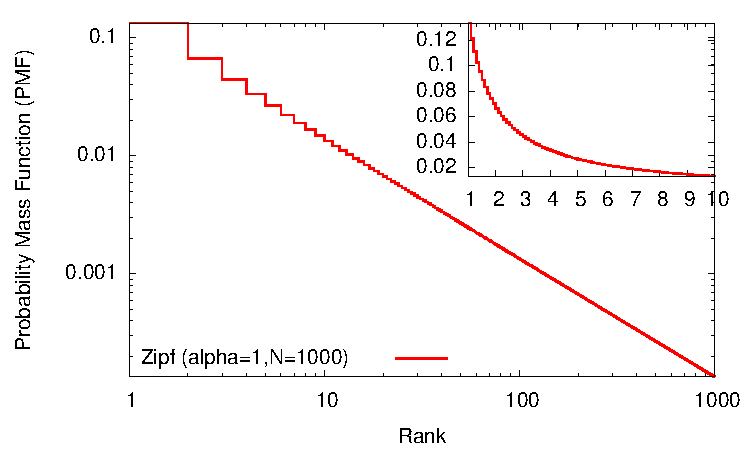
\includegraphics[width=0.45\columnwidth]{./diagrams/powerlaw-zipf}
    }\qquad
    \subfloat[][Pareto distribution: This follows the 80-20 rule, where 80\% of the function's weight is within the top 20\%] {
        \label{fig:dist_pareto}
        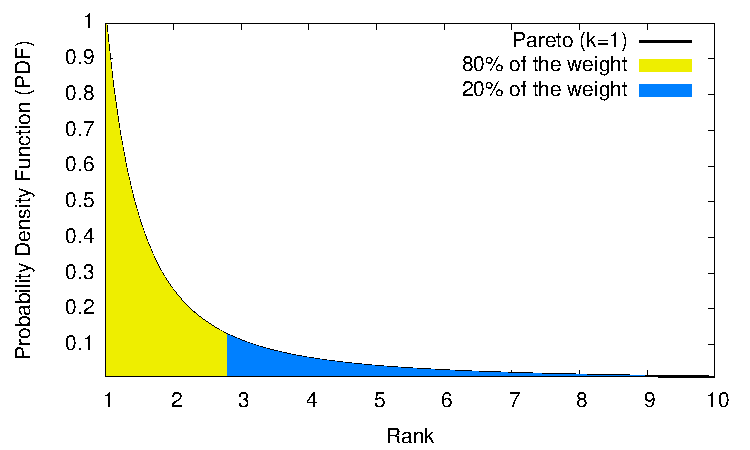
\includegraphics[width=0.45\columnwidth]{./diagrams/powerlaw-pareto}
    }

    \caption
        {Probability density functions for Zipf and Pareto distributions}
    \label{fig:dist}
\end{figure}

%   "Temporal Locality: accesses to videos also exhibit strong temporal locality. If a video has been accessed recently, chances are that it will be accessed again soon."~\cite{acharya2000cua}

%   "Our analysis found that of the 23,738 media objects referenced, 78\% were accessed only once. Only 1\% of the objects were accessed by ten or more sessions, and the 12 most popular objects were accessed more than 100 times each."~\cite{chesire2001maa}.

    The popularity of content within a VoD system play an important role in deciding how it is cached and replicated. Popularity of web objects typically follow a Zipf-like distribution. Within Zipf distributions~\cite{zipf1949hbp}, the popularity of a object is proportional to its rank, \emph{i.e.} the $i$\sth most popular object receives $1/i^\alpha$ of requests, as seen in \autoref{fig:dist_zipf}. This implies the majority of content is unpopular, and a few items are extremely popular, making up the weight of the distribution. This is be illustrated by observations made by Chesire~\emph{et~al}. Out of 23,738 video objects, 78\% of which were only accessed once, 21\% accessed two to nine times, and the remaining 1\% accessed ten or more times, with the 12 most popular objects being accessed more than 100 times each~\cite{chesire2001maa}.

    Video-on-demand popularity was first suggested to follow a Zipf distribution by Dan~\emph{et~al.} in 1994~\cite{dan1994spf}. This was again observed by Wolf~\emph{et~al.} in 1997, however with varying degrees of skew each week~\cite{griwodz1997ltm}. In early 2000, Acharya~\emph{et~al.} could not fit the popularity of their education videos to a Zipfian distribution~\cite{acharya2000cua}. Instead they noticed requests to their objects were more biased towards the popular titles than expected within a Zipf distribution. This bias can be explained by Cherkasova and Gupta's analysis of an enterprise media workload~\cite{cherkasova2002cle}. They observed that over long timescales the bias towards the most popular items increased. For example, object popularity fitted a Zipf distribution with $1.3 \leq \alpha \leq 1.6$ over 1-month periods, over a 6-month period with $\alpha=1.6$, and eventually Zipf did not fit well over a year.

    The fact that Zipf did not fit well over a year time scale is often overlooked and the reasons for this are typically misunderstood. Zipfian models are useful for static distribution, those which do not have a temporal component. For example, Zipf was first developed by George Kingsley Zipf when studying the frequency of words appearing in a corpus of natural language. The corpus would not change over time, \emph{i.e.} words would not be added or removed. This differs from popularity of videos over a timescale as it is common for new videos to be added and removed over time, and for the popularity of the videos to change over time. Instead the Zipf models should be used to model the popularity over shorter periods, such as daily or weekly, or be used to blindly model the rank of objects on daily bases. For example, objects on a daily bases may follow a Zipf distribution, but instead of noting the popularity of each object, note the popularity of each rank. This will then more accurately model the expected popularity on any given day, and is more useful for the design of caching systems.

    % Maybe mention why web objects are requested multiple times (ie they change)

    Whilst analysing Kazaa's~\cite{kazaa} peer-to-peer traffic, Gummadi~\emph{et~al.} proposed a new distribution that fitted the popularity of objects better than Zipf~\cite{gummadi2003mma}. Individual Kazaa users rarely requested the same object twice, unlike in web traffic where the same object may be requested multiple times by an individual. This lead to the ``fetch-at-most-once'' model, which fitted better to the workloads discussed by Cherkasova and Gupta~\cite{cherkasova2002cle}, as well as ranking data collected from video store rentals~\cite{vsm}, and box office sales~\cite{imdb}. This model says that users fetch objects following a Zipf distribution, but must not request the same object twice. If the user chooses a previously fetched object, then a new object is picked again from the Zipf distribution.

%\todo{Find who compared fetch-at-most-once to video rentals}

    Yu~\emph{et~al.} contradicted the fetch-at-most-once model when analysing a 219 day trace collected from a VoD system deployed by China Telecom used by 150,000 people~\cite{yu2006uub}. Their object popularity fitted best to a Zipf distribution, except for a long heavy tail. They speculate that their results do not fit the fetch-at-most-once model because users were unable to save the viewed media, thus if they wished to watch a video again, they had no choice but to re-fetch it.

    Which model is best seems to depend on how the videos are accessed, what genre of video they are, and other currently unknown factors. However Cha~\emph{et~al.} tried to explain the shape of the distributions through simulation~\cite{cha2007tyt}. A fetch-at-most-once model was simulated with a Zipf distribution of $\alpha=1.0$. Parameters such as the number of users, the number of requests per user, and the number of objects were varied. They found that the effects of fetch-at-most-once are barely noticeable when there are few requests, this intuitively makes sense as there is less chance of selecting the same object twice. The number of users did not seem to impact the shape of the distribution at all. When the number of objects increased, the effects of fetch-at-most-once were also reduced, again, because the chance of selecting the same object is decreased.

    Both Zipf and fetch-at-most-once are categorised as power-law distributions. However there are other factors which govern the power-law nature of these distributions. In most of the analysed models, the two ends of the distributions have been truncated or extended. It is suggested by Chris Anderson that ``Latent demand for products ... is suppressed by bottlenecks in the system''~\cite{anderson2006tlt}. Take, for example, the popularity of movies in cinemas. Most cinemas show the most popular movies, however there are few cinemas screening niche content. This causes the popularity distributions of the movies to have a truncated tail. This is refereed to as a ``distribution bottleneck'', where due to lack of distribution, the tail is truncated. The opposite can be true, where, for example, there is ample supply of niche content, but it is hard to find this niche content, thus a ``information bottleneck'' exists~\cite{cha2007tyt}.

    %TODO Perhaps a last paragraph to summarise?

\subsubsection{Popularity Over Time}
\label{sect:pop_over_time}
%    Popularity is greatly changed by top-ten lists~\cite{yu2006uub}
%    Popularity changes each day as new content is added~\cite{paneda2006pav}
%    The content is divided into many groups: "Short life", "Long life", "Up and down", "Seasonal"~\cite{paneda2006pav}
    Over time the popularity of videos will change, greatly impacting the decision on what to cache or replicate. It is essential to consider how frequently replication updates are carried out. Too often and video may needlessly be moved, but too infrequent and the servers may not be prepared for demand of a newly popular video. As such the rate of change in user interest can aid in the design of a VoD system.

    Paneda~\emph{et~al.} noted the popularity of videos on a popular Spanish news website would change daily as new content was added. Typically the most popular items for each day were added to the site on that day. However after the first day the content could be grouped into four categories; \emph{short life}, \emph{long life}, \emph{up and down} and \emph{seasonal}. Short life content would reach its peak popularity on the first day, and after the first day the number of accesses would decrease suddenly. Long life content also peaks on the first day, however its popularity decreases slowly over the the following days/weeks. Up and down content, will build up popularity for a few days, and then decrease in a similar way to long life. Finally, seasonal content would have peaks in popularity every few weeks or months~\cite{paneda2006pav}.

    In a study of a enterprise media server, Cherkasova and Gupta observed that on any given month most of the bytes transferred were for new content. They found that \verb+~+50\% of requests to content were made in the their first week, with and addition 20\% to 30\% being made in the following four weeks~\cite{cherkasova2004aoe}. They did not discuss if they found seasonal or \emph{up and down} style content. However these patterns may be directly related to the genre or appeal of the content.

    Yu~\emph{et~al.} took a different approach to monitoring popularity over time in their large scale VoD system~\cite{yu2006uub}. They looked at the rate of churn in the top-10, top-100, and top-200 most popularity movie charts over different time scale. They began by looking how newly inserted content affected these top charts on a hourly timescale. The time content was added to the system, correlated with a high change in user interest. This encourages that newly added content be replicated early to avoid insufficient availability.

    It was also noted, that over a small time scale, \emph{i.e} hours, the top-10 list had a small amount of churn averaging around 25\% change per hour, whereas the top-100 and top-200 experienced 45\% change per hour. Over longer timescales such as days and week, it was found that the top-10 list rarely remained stable, whereas the top-100 changed only 15\% each day.

    The main observations from Yu~\emph{et~al.} suggest that popularity changes on different timescales, with the top-10 being stable for a day, and the top-100 being stable over longer periods. It is suggested that a two level caching model be used, with a small adaptive cache for the top-10, and larger more constant cache for the top-100~\cite{paneda2006pav}.

    Although popularity of objects change over time, it appears these changes are very specific to the viewing population and genres of the objects. In the current research no single model has been found which accurately explain the observed behaviours, however, it is clear that this is an important metric for cache design.

\subsubsection{Recommendations}

% TODO Fix the below paragraph
    Some systems display a top-10 list of the most popular videos that month, or a list of recommendations, such as new releases, or videos a user may find of interest. All of these lists can greatly influence what a user views. However, the importance of recommendations has not been studied, much, it has been highlighted as a great source of revenue for companies such as Amazon~\cite{anderson2006tlt}.

    Yu~\emph{et~al.} have studied this phenomenon more analytically when they observed it in their VoD system. They found one video stayed in the top-15 most popular film list for a significant amount of time, but once a administrator manually removed the film from the list, its popularity quickly declined~\cite{yu2006uub}, and never recovered.

    The fact that users appear influenced by these lists, can play in the favour of a video-on-demand system. For example, if it is know ahead of time that a film will appear in the list, the system can take necessary steps to ensure the content is well replicated, in advance of the demand.

%This factor can also impact the results later shown in this thesis. We displayed a list of bookmarks to the user, and found them to be very popular.

\subsubsection{Session duration}

    The session duration can be defined in two ways; firstly the duration a user spends using a Video-on-Demand application, and secondly the duration the user spends watching a particular video. Each definition is applicable in different contexts. For example, knowing how long a user views a single video can aid in caching decisions, whereas knowing how long a user uses an application can aid in the design of the application. This section is only interested in how long a user views a particular video for.

    From early studies on VoD it has been observed that session duration is quite short. For example, in 2001, whilst studying streaming traffic on a large university campus, Chesire~\emph{et~al.} showed that 85\% of all sessions lasted less than 5 minutes with a median session duration of 2.2 minutes. This is compared to a mean advertised media length of between 2.5 and 4.5 minutes. Long lived sessions (those longer than one hour) accounted for only 3\% of all client sessions~\cite{chesire2001maa}.

    Almeida~\emph{et~al.} found similar results when analysing logs from an educational media server. A significant proportion of requests were less than 3 minutes in duration. These sessions were very short when compared to the length of the media, which had a median length of 60 minutes~\cite{almeida2001aem}.

    %Padhye and Kurose also looked at an educational media service, which provided HTML lecture slides, accumplied with audio narration. The session direction of

    It was suggested by Guo~\emph{et~al.} that the short duration was due to the long wait times, and low patience of users~\cite{guo2005amw}. Yu~\emph{et~al.} found that short durations within their traces were due to users sampling the media by ``scanning'' through them. An inverse correlation was also found between the session lengths and the popularity of the media. Less popular videos actually had longer session times~\cite{yu2006uub}.

    As noted by Guo~\emph{et~al.}, 20\% of network bandwidth was wasted buffering video which was never watched due to the user aborting the stream~\cite{guo2005amw}. These short session durations encourage the design of agile systems which can quickly display the media before the user becomes impatient, as well as techniques such as prefix caching~\cite{sen99ppc}, which prioritise caching of the first frames of the media for quick delivery.

\subsubsection{Interactivity}

    % Describe what interactivity is, and why its important
    % Few people interact
    % longer files have more interactivity, also with longer files more forwards are noticed, and less pauses

    % Pause is the most common
    % Jump forward and back are equally popular

    % TODO Find that paper with short/medium/high interactivity levels

    The playback of media is not always passive; certain systems allow for interactive control over the playback. For example, the user may be able to pause, fast-forward or rewind, as well as seek to arbitrary points within the content. Offering interactive features can be challenging. For example, most multicast delivery techniques require all clients to be at a similar playback point within the stream. However, if a client seeks arbitrarily, they are no longer at the same playback point, and thus must join another multicast group, or start to receive the content via a different delivery method. As such, an understanding of how users interact with the content can be invaluable for good delivery.

    There have been few studies on how users interact with media. This may be due to the relatively few systems which have interactive features. However, Huang~\emph{et~al.} found then when interactive controls were available, for videos clips shorter than 30~minutes, only 20\% of all sessions showed interaction from users~\cite{huang2007civ}. Unsurprisingly, the longer the video, the more interactivity is observed. For example, with videos less than a hour in length 40\% of session exhibited interactivity. This trend is consistent with the results within this thesis, and other research~\cite{costa2004aci}. However, this thesis presents results with far higher percentage of sessions with interactivity. This may be due, in part, to the novel interface presented to the users which encouraged interactivity.

    Costa~\emph{et~al.} found that when users do interact, that in both education and entertainment the most common action is pause~\cite{costa2004aci}. This was confirmed by Vilas~\emph{et~al.} who noted that 7\% of session for short videos (those less than 5 minutes in length) and 10\% of longer videos session had at least one pause. It was also shown that the pause duration could be modelled with a Weibull distribution, with means of 55 seconds and 95 seconds, for short and long videos respectively~\cite{vilas2005uba}.

    Another common action is seeking forwards or backwards. For short videos, the percentage of forward and backwards seeks appeared to be roughly the same. However as video length increases, there are more forward seeks, indicating users wished to skip ahead~\cite{almeida2001aem}. Seeking forward also surprised Padhye and Kurose when studying an education server which provided lectures. They assumed students would regularly seek backwards to go over a section again, but found that seeking forward was seven times more popular than seeking backwards~\cite{padhye1998esc}.

    Vilas~\emph{et~al.} modelled the number of seeks per session, and follow it matched a Zipf distribution, with $\alpha$ values between $3.73$ and $5.8$~\cite{vilas2005uba}. This implies that most users never sought backwards or forwards, however when users did, they did so numerous times.

    %\todo{A paper somewhere talks about bursts of seeks, and then long playbacks, and then a burst again}

    The distance sought was also studied by Padhye and Kurose, who observed on their education server a very large average distance. For forward seeks this was approximately 35 minutes, and backward was 34 minutes, for media around 70 minutes in length. However, one third of these seeks were for less than 3 minutes~\cite{padhye1999cmc}.

%\todo{Talk about ON/OFF time analysis}

%    7\% of short video sessions had 1 or more paues, and 10\% of long videos had 1 or more.~\cite{vilas2005uba}
%    Pause length 55.7s and 95s for short and long respectivitly
%    Shows slightly more forward than back jumps

%    short videos (0-5 min)
%    long videos (5-50 min).
%
%    Forward (short videos) Zipf ? = 5.8 = mean 1.0226
%    Forward (long videos) Zipf ? = 4.32 mean 1.0808
%    Backward (short videos) Zipf ? = 4.32 mean 1.0808
%    Backward (long videos) Zipf ? = 3.73 mean 1.1469
%
%Forward (short videos) Weibull alpha =0.16827 beta =0.45321 mean 124.4929s
%Forward (long videos) Weibull alpha =0.10916 beta =0.54129 mean 104.4828
%Backward (short videos) Weibull alpha =0.09058 beta =0.47459 mean 348.7646
%Backward (long videos) Weibull alpha =0.059598 beta =0.59236 mean 178.7992
%
%    During periods of approximately stationary request arrival rate, the BIBS client session arrival process is approximately Poisson, whereas the time between interactive requests within eTeach sessions is more accurately modeled by the heavy-tailed Pareto distribution, as has been found in more traditional Web server workloads [3,16, 19].~\cite{almeida2001aem}
%
%    Fast forward and rewind operations are extremely rare in eTeach (i.e., less than 0.5\% of all requests in the logs)~\cite{almeida2001aem}
%
%    "For short files, jump backwards is the most common client interaction. For larger file sizes, pauses become more frequent"~\cite{almeida2001aem}
%
%    "Pause is, by far, the most common client interaction in the video workloads. Jump backwards and jump forwards are roughly equally frequent for longer videos."~\cite{costa2004aci}
%
%    Unsurprisingly longer files have more interactive requests~\cite{costa2004aci}
%
%    "As file size increases, the percentage of pauses decreases, and the percentage of jump forwards increases. In other words, clients tend to skip more uninteresting file segments as they watch longer videos. The frequency of jump backwards remains roughly stable across all file size ranges in both workloads"~\cite{costa2004aci}
%
%    "a client usually interacts with the video in the same way repeatedly"~\cite{costa2004aci}
%
%    "average jump distances in either direction increase with file sizes"~\cite{costa2004aci}

\subsubsection{Segment Popularity}

%    For the most frequently accessed files in eTeach, all ten-second segments of the media are accessed nearly equally often, whereas for less popular files, the access frequency is higher for earlier segments of the media.~\cite{almeida2001aem}

%    "It is roughly uniform for the most popular files (usually lectures above 15 minute long), as shown in Figure 12-a, and skewed towards early segments for less popular files, as in Figure 12-b."~\cite{costa2004aci}

%    "If it is roughly uniform (as in Figure 12-a), a single (file) measure is enough to capture the distribution of segment access frequencies, and full file caching is the best strategy for unicast delivery. In the cases where a skewed distribution was found, the curve is usually well behaved (as shown in Figure 12-b) and can be roughly approximated using only two or three measures."~\cite{costa2004aci}

    When users seek, not all segments of the video may be viewed equally. This could lead to some segments being very popular, whereas others unpopular. This situation can also be caused if users do not watch for the full duration of the video. This all has implications on how media, or segments of the media should be cached.

    Almeida~\emph{et~al.} divided education media into ten-second segments. For the most popular video, all segments were accessed roughly equally, however for the less popular video, the earlier segments within the media were accessed more~\cite{almeida2001aem}. This indicates only the beginning of the content was viewed. Costa~\emph{et~al.} also observed this result with newer education content, as well as entertainment content~\cite{costa2004aci}.

    When Huang~\emph{et~al.} analysed the traces from a large entertainment Video-on-Demand site, they found users would regularly quit before the end of the video. For short videos, most users watched for the full duration, however as the video length increased users were more likely to stop early. For example, with videos less than 30~minutes in length, only 18\% would watch for the full duration, with 22\% watching for 60\% of the duration~\cite{huang2007civ}.

    % A similar finding was made by Cherkasova and Gupta when they observed

    These later results are consistent with the findings in this thesis, however, we noted areas of high interest dubbed \emph{hotspots}. The previous work found only minor differences in segment popularity, whereas we found segments with orders of magnitude different popularity. This result is speculated to be because of the higher levels of interactivity found within this thesis' traces.

\subsection{Live Streaming}

% vandermerwe2002svt     Streaming video traffic: Characterization and network impact
% veloso2006hcl          A hierarchical characterization of a live streaming media workload
% sripanidkulchai2004als An analysis of live streaming workloads on the internet
% li2005csm              Characteristics of streaming media stored on the Internet
% chesire2001maa         Measurement and analysis of a streaming media workload
% costa2004aci           Analyzing client interactivity in streaming media

%   In such an environment, users are mostly �passive�; they are fairly limited in how they are allowed to interact with objects: they can only join or leave the audience of the live �active� object."~\cite{veloso2002hcl}

    % Nic has read below

    The characterised workloads of live streaming are likely to be different to those of video-on-demand for a couple of reasons. Firstly, users are mostly passive in live streaming, fairly limited by how they can interact with the media. In some cases, pause is available, but seeking is typically not. The only real interaction available is the choice of when to join or leave the stream. Also, as all users are viewing the same content, the force of the crowd may be stronger, for example, all user leaving simultaneously as a live programme ends.

    Secondly, in a 2004 study of a large CDN, it was found that only 7\% of streams were video, accounting for only 1\% of all requests~\cite{sripanidkulchai2004als}. The remaining streams were audio only, for example, radio stations. This section highlights the differences between VoD and live streaming workloads, while explaining any features specific to live streaming.

%\subsubsection{Popularity - Both VoD and Streaming}
%    \todo{start/finish}
%
%        "The distribution of client requests to objects (in both VoD and Streaming) is Zipf-like, with a alpha parameter of 0.47."~\cite{chesire2001maa}.
%
%        "Accesses to pre-recorded, stored media objects are user driven;3 they are directly influenced by user preferences� namely, what to access and when to do so. Accesses to live media are object driven; they are directly influenced by aspects related to the nature of the object�e.g., show/event time, activities captured by various feeds, etc. In such an environment, users are mostly �passive�; they are fairly limited in how they are allowed to interact with objects: they can only join or leave the audience of the live �active� object."~\cite{veloso2002hcl}

%    \subsubsection{Popularity}
%        The popularity distribution is Zipf-like with two distinct modes~\cite{sripanidkulchai2004als}.

\subsubsection{Time-of-day}

    % Non-stop streams had daily periodic access patterns
    % Patterns followed user's timezone
    % Short streams however did not follow any time-of-day access
    % Short streams did however always start with a flash crowd. Indicating object driven requests
    % Almost 50\% of non-stop streams also had flash crowds, on some days.

    Non-stop streams have a diurnal access pattern, peaking at the same time each day. This kind of diurnal access patterns has not be observed with Video-on-Demand. It is speculated by Veloso~\emph{et~al.} that diurnal access patterns are smoothed out because the clients have control over when they access the media and by clients accessing from multiple time zones~\cite{veloso2006hcl}. The non-stop stream is also influence by time zones, but less so, for example, Sripanidkulchai~\emph{et~al.} observed for a single radio station's stream, several similar periodic patterns were present, but shifted by the time zone of the clients~\cite{sripanidkulchai2004als}.

%Nic has read below

    Streams with a short durations did not follow the same daily pattern. However, nearly all short stream began with a \emph{flash crowd}. A flash crowd is a sudden surge of users all wishing the view the same content. This typically overwhelms servers, and results in an accidental denial of service. These types of events are certainly \emph{user driven}, with users specifically joining the stream for an event. Almost 50\% of non-stop streams also exhibited a flash crowd event every few days. This, for example, could be the result of many users joining a radio stream to listen to a popular programme~\cite{sripanidkulchai2004als}. This behaviour is rarely seen in VoD systems, as the requests are \emph{object driven}.

\subsubsection{Session duration}
%Nic has read below

    Session durations for live streaming follow that of video-on-demand. Most sessions are short, with a a few long-lived sessions. Vandermerwe~\emph{et~al.} found the distribution of session duration to be long-tailed, with 69\% of sessions being less than 2~minutes in length, 88\% less than 10~minutes, and the top 8\% being longer than 20~minutes~\cite{vandermerwe2002svt}. These results were similar to Chesire~\emph{et~al.} who found a similar long-tailed distribution with their top 3\% of the population being more than a hour in length. However, these 3\% of long-lived sessions accounted for about half of all bandwidth consumed~\cite{chesire2001maa}. This demonstrates how the distribution is not just long-tailed, but heavy-tailed.

    Sripanidkulchai~\emph{et~al.} compared the session durations of live streaming content, repeating streaming content and video-on-demand content. The repeating streaming content consisted of non-stop streams which broadcasted the same programme over and over, for example, every 30~minutes. The session duration for both repeating streaming content and the VoD content exhibited similar ``truncated'' Pareto distributions. The majority of sessions with this distribution are short, with the few long-lived sessions being no longer than the content's length. However, the session durations for live streaming content, fitted a Pareto distribution with a heavy tail. This extended long tail is caused by the user's actions, rather than being truncated arbitrarily by the content's length~\cite{sripanidkulchai2004als}.

% ~\cite{chesire2001maa}
% Although the long-lived sessions ( > 1 hour) account for only 3\% of all client sessions, these sessions account for about half of the bandwidth consumed by the workload

% ~\cite{vandermerwe2002svt}
% A large proportion of the sessions (69\%) are on for 2 minutes or less. However the distribution exhibits a long tail About 12\% of the sessions are at least 10 minutes long, while 8\% of the sessions are longer than 20 minutes.

% ~\cite{sripanidkulchai2004als}
% Session duration distributions are heavy-tailed. The tails have 3 distinct shapes corresponding to 3 types of streams: nonstop with fresh content, non-stop with cyclic content, and short streams.

\subsubsection{Interactivity}
%Nic has read

    As far as we are aware there have been no studies on the characterisation of interactivity with live streaming. This will of course be due to the lack of interactive controls. For example, it is impossible to seek forward in a live stream, and only possible to seek backwards if the stream has been stored by the server or client.

    The storing of live streams by the client is becoming increasingly popular with the use of \emph{time-shifting} devices such as digital video recorders (DVRs) or personal video recorders (PVRs). These are typically set-top boxes which buffer broadcast TV. The user is then able to pause while the box continues to buffer, or rewind within the buffer. Additionally, the user may fast-forward to catch up with the stream if they have paused or rewound. PVRs are discussed in more detail in \autoref{sect:pvr}.

    As far as this author is aware, there have been no research examining how users interact with PVRs. However, it is commonly reported that these devices are used to fast-forward through advertising when watching recorded programming~\cite{barwise2005ffp}. When users skip adverts, these advertising segments become less popular than the rest. This has implications for how these segments would be cached or replicated.

%    "More than half (57\%) of all UK residents �time-shift� their TV viewing, using on-demand TV services or recording live television for viewing later", "36\% use a PVR"~\cite{YouGov2008red}

\subsection{Implications}

%Nic has read

%    "Such insight is useful for system design, evaluation, planning, and management"~\cite{sripanidkulchai2004als},

%    "Therefore, system caches can maximize their effectiveness by allocating the majority of their capacity to storing beginning segments of movies." ... "Clearly, VOD systems need to exploit time-varying user interest patterns by intelligently partitioning videos into segments and taking their time index in replica and cache management."~\cite{yu2006uub}

    This section has highlighted the main characterisation models for both video-on-demand and live streaming. Understanding how media is consumed has many practical uses, such as designing, evaluating, planning and managing systems. This is especially true when dealing with highly interactivity workloads, as these typically cause excessive load for servers.

    It is clear that starting with a metric as simple as content popularity can greatly aid in replication and caching strategies. As popularity is typically modelled by a power-law distribution, systems will benefit from caching the most popular content. However, as distribution bottlenecks are reduced, and users find it easier to access their niche content, it might be useful to implement multi-level caching hierarchies, which can use different policies based on the the ranking of the content. For example, one caching policy can be used for most popular content, whilst another can be used for the more niche content. As such, the niche caching policy may only store the content in local caches for a short, whereas the very popular content is kept available for a longer period of time, on a more global scale.

    Knowing what is popular, and caching it, is a reactive method, however, it is sometimes useful to be proactive. This may be possible if the content is listed in top-x charts, such as the top-10 voted movies. The popularity of an object ranked 10\sth, is far higher than that at position 11, when only the top-10 chart is available to the user. The effect these charts have on the user's viewing habits can easily be exploited by the video-on-demand system. As soon as the chart is available, the system can begin pro-actively replicating the content, perhaps near to the target demographic.

    It is also clear that certain content has a seasonal or recurring monthly appeal, such as Christmas-themed videos. Again, these can be pro-actively replicated ahead of demand, at the cost of potentially wasting resources. Other content is perhaps only popular for a very short time, such as daily news reports. Understanding the appeal of the media can greatly help choose on the appropriate content management techniques.

    Where interactivity is concerned, it is already clear that users can be impatient and either scan through the content, or prematurely stop playback. Therefore, to maximise caching efficiently, the first segments of media can be stored in preference to the later segments. Techniques such as prefix caching~\cite{sen99ppc,hofmann1999cts} can also aid in deciding which segments are the most useful to cache and replicate.

    Even though users do interact with the content somewhat, high levels of interactivity have not previously been reported. However, the results presented later in this thesis (see \autoref{chap:evaluation}) show much greater levels of interactivity. Different design decisions must be made under these workloads, which will be discussed later in the thesis.

     %When high levels are observed, there are many other implications for the system, which do not apply to the previously observed low-interactivity workloads. This includes caching sparsely distributed segments within the content, such as a popular scene in a movie or a point of interest in a sporting event, for example, a goal.

%\section{Workload Generators}
%    Discuss what workload generators exist. What kind of models they assume, and their limitations.

% An Empirical Study of RealVideo Performance Across the Internet - Looks at quality of stream due to the internet


    \chapter{Interactive Video-on-Demand~System}
\label{chap:experiment}

\begin{figure}[t]
    \centering

    \subfloat[][System setup]{
        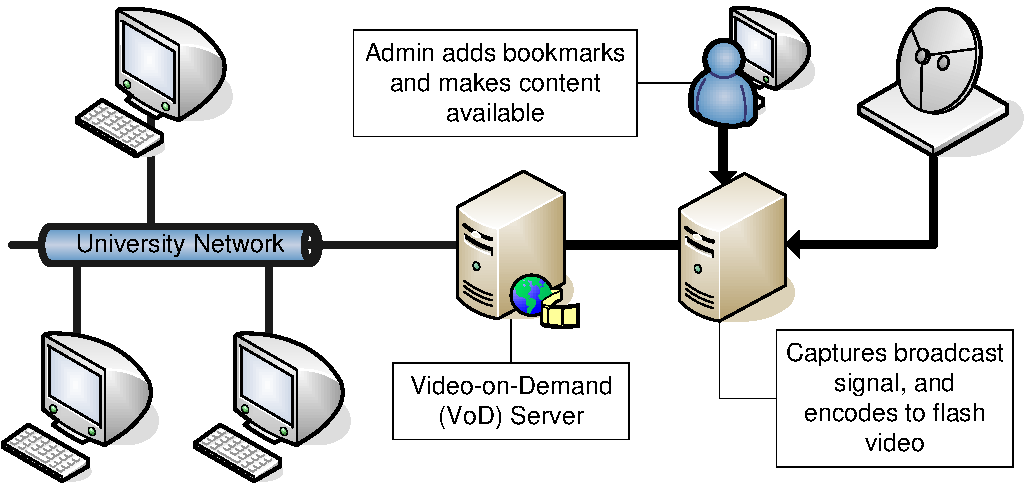
\includegraphics[width=0.5\columnwidth]{./diagrams/setup}
        \label{fig:system_setup}
    }
    \subfloat[][Player interface] {
        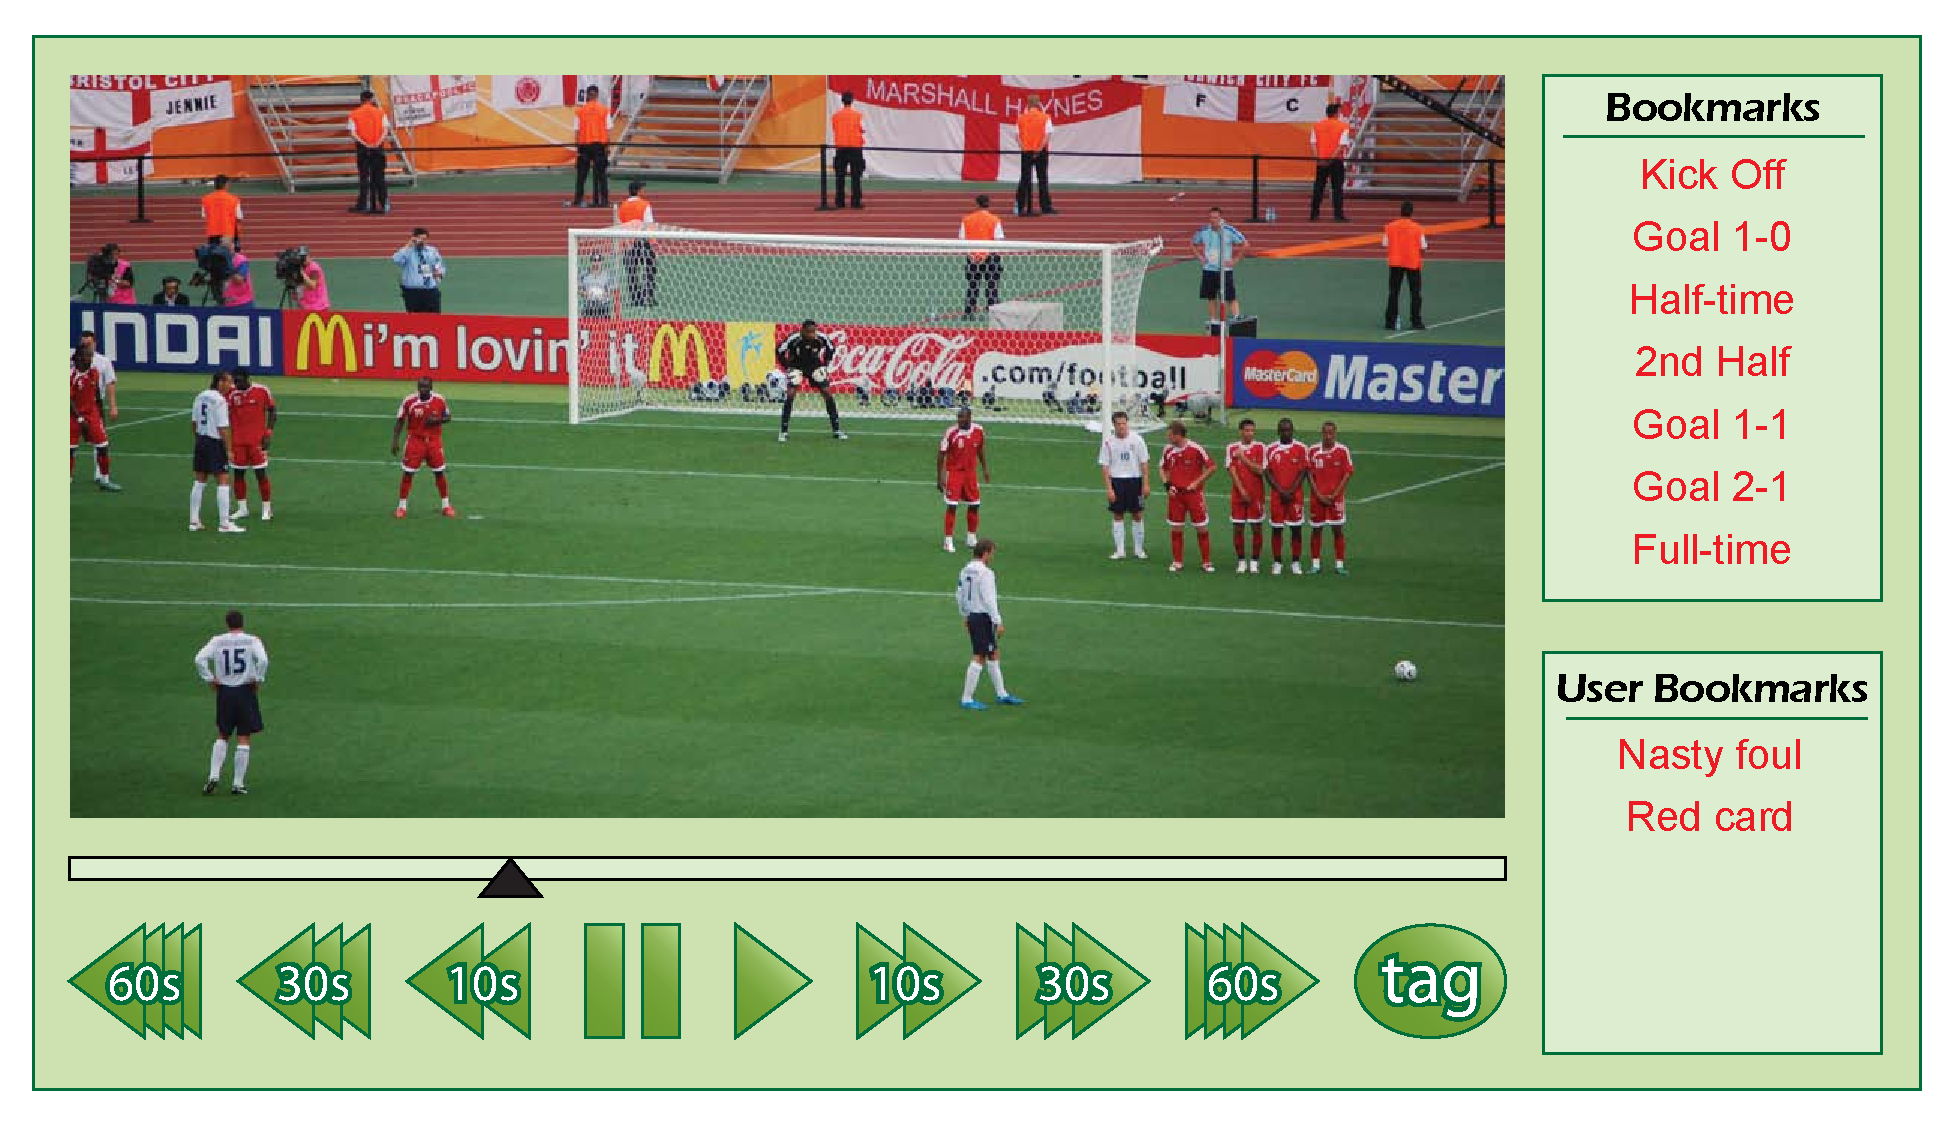
\includegraphics[width=0.5\columnwidth]{./diagrams/Interface}
        \label{fig:interface}
    }

    \caption{Diagrams of our video-on-demand system}
    \label{fig:system}
\end{figure}

There has been lots of work on characterising user behaviour when viewing video-on-demand (VoD) and streaming media (as discussed in \autoref{sect:characterisations}). However, there has been little analysis when a highly interactive system is used, for example, a system where users regularly pause and resume playback and actively seek around the media. This would generate results which would be a complete departure from the classic start-to-end model.

To obtain traces from a highly interactive workload, we set up and designed a video-on-demand system. This system was designed to provide powerful, yet simple interactivity controls, which would hopefully encourage more interaction between the users and the system. Once deployed, the system would be used to record traces of real user behaviour, and to be used as a test environment for future experiments. To be useful, the system had to meet three criteria:

\begin{description}
  \item[Wide user base] So that we could maximise the number of participants, the system needed to be designed in a way which was non-invasive, and simple for the users to use. This ruled out installing any special software on the users machines.

  \item[Encourage Interactivity] To ensure that the system generates a highly interactive workload, the layout of the user interface should make it easy to pause, resume, seek, \emph{etc.} This should be supported by the system, which should offer these features with low-latency, as to not to discourage their use.

      The content chosen for the system is also important. It should somehow encourage the use of interactive controls, for example, feature films will always be viewed start-to-finish, but genres such as sports may encourage users to view just the highlights.

  \item[Simple and Cheap] Finally, to ensure this system could be deployed, it has to be simple and cheap, for both us and the users. This of course can be achieved by using ``off the shelf'' products. Open source software would also be useful as it can easily be customised for our needs.

\end{description}

To meet all these requirements, the following choices were made. The system should be a simple client-server Flash based one, similar to the ones described in \autoref{sect:ugc}. These sites are relatively simple to set up and easily customisable. They also allow for a wide user base, as they use a simple web browser and the Flash player, both of which are commonly found on users' PC. These technologies will also typically work through firewalls, unlike other streaming protocols. This was beneficial to us, as it allowed us to stream to restricted users on our university campus.

The Flash player expects the video to be encoded as an FLV file; this can easily be achieved using the open source FFmpeg~\cite{ffmpeg}, which again makes this system simple and easy to deploy. One issue with the Flash player was the lack of seeking support, however a \emph{hack} was developed to add this functionality. The exact description of how this hack worked is described in \autoref{sect:seekable_flash}.

We chose a few different genres of content, but for the first round of experiments we served the 2006 FIFA World Cup. This is a hugely popular event with three to four matches on each day. Due to the number of matches each day, many users would miss the live match; this therefore encourages them to use our site to view any matches they missed.

The majority of videos served by our system typically had areas of particular interest, such as goals. To allow users to quickly navigate, we designed and added a \emph{bookmark} feature. While viewing the videos, the users were shown a list of bookmarks to the key events within the content. Then, at any point, the user could click the bookmark to instantly seek to its position within the media. Within our sport content, for example, goals, fouls and similar occurrences were bookmarked.

The concept of bookmarks in media is not new. Most DVDs contain chapter and scene bookmarks, which enable the user to start playback at any location. However, as far as we are aware, there have been no studies on how these DVD features are used. If a user does start a DVD at a specific chapter, it is no technical challenge for the DVD player to seek to the correct point and begin playback. This is not true for video-on-demand, as it can be quite strenuous for servers to seek arbitrarily. As such, the analysis of bookmark use within VoD will be novel.

The rest of this chapter explains how our video-on-demand system was designed and deployed to cater for our interactive experiments, and also outlines the different content used. This also includes the design of different tools to enable seeking within Flash videos.

\section{System Overview}

We set up a simple, interactive video-on-demand system. The system was divided into three main components: the capture server, the Video-on-Demand server, and a web interface as depicted in \autoref{fig:system_setup}.

% The capture server

Our capture server recorded publicly-broadcasted raw MPEG-2 streams of the programmes selected for our experiments. The recording was done via a digital TV capture device, using VLC~\cite{vlc} to store the raw stream. Once the full programme had been recorded, the system transcoded the stream with FFmpeg~\cite{ffmpeg}. Two streams were created; high and low bitrate Macromedia Flash 7 FLV files (1~Mbps and 300~Kbps respectively). Administrators would then manually add metadata to the system describing the files. This metadata included the title and description of the video as well as marking the location of key events within the videos which would become \emph{bookmarks} (more details on what was bookmarked is listed in \autoref{sect:experiment}). The final FLV files were then transferred to the VoD server, making them accessible to the users. The full procedure described typically took around twice the length of the recorded video, and so the videos were available shortly after being aired.

% VoD Server
The VoD system was an Apache webserver, which served the Flash-based user interface over HTTP. This server was only accessible to staff and students within Lancaster University's campus, and those staff and students connecting remotely via the university's Virtual Private Network (VPN). To aid in logging, all requests made through the user interface were verbose, allowing us to determine exactly which controls users pressed and when. Additionally, each playback window would maintain a periodic (10~second) HTTP-request heartbeat with the server, which was used to determine when connectivity was unexpectedly lost.

To handle user tracking, each user was assigned a unique session ID, which was stored within a HTTP cookie and their URLs. Each event that was logged contained this identifier, allowing us to track individual users throughout their visit to the site. If, however, a user blocked or deleted their cookie, they would appear to be new to the system upon each visit. We note within our analysis where this uncertainty could affect the results.

% Web interface
The web interface consisted of two main sections: an index page allowing the user to select any available video from the system, and the player interface that displayed the video (as shown in \autoref{fig:interface}). We were aware that the user interface would constrain the users' actions somewhat, and it was therefore designed to be as simple and generic as possible. We also wanted the interface to offer modern interactive controls (also called \emph{trick-modes}).

There are many different trick-modes, for example the ability fast-forward or rewind, or the ability to step through the video one frame at a time. However, offering too many trick-modes would clutter the interface, and most of them wouldn't be useful. Therefore, we limited the interface to having just seeking controls (\emph{e.g.} forward, backwards and to arbitrary points), as well as pausing and resuming.

Forward and backward buttons were provided that allowed seeking 10, 30 and 60 seconds in either direction. As these are relatively short distances, we also provided a \emph{seek bar} which enabled users to seek to any arbitrarily chosen time. Finally, a list of \emph{bookmarks} was displayed to the users, which enabled them to jump directly to key events. Bookmarks were added by an administrator, but later the interface was extended to also allow users to submit their own bookmarks (via the \emph{tag} button), which other users could see and use. User bookmarks often covered events that were not typically bookmarked, but were of particular interest (such as events that came under later scrutiny).
%
%\section{Logs}
%
%To analysis the behaviour of users of the system, numerous logs files were generated and later parsed. This section gives a brief overview of the log files, and how they were analysised.
%
%\begin{flushleft}
%\footnotesize
%
%[17-Jun 03:24:27] log.php?why=restart\&user=a044cb\ldots\&startBytes=0\&startTime=0\&seconds=0\&file=arg-scg\&action=seek
%
%[17-Jun 03:24:30] log.php?why=shortcut Goal 1-0\&user=a044cb\ldots\&startBytes=176378857\&startTime=1297\&seconds=1301\&file=arg-scg\&action=seek
%
%[17-Jun 03:24:37] log.php?user=a044cb\ldots\&seconds=1304\&file=arg-scg\&action=alive
%
%[17-Jun 03:24:47] log.php?user=a044cb\ldots\&seconds=1314\&file=arg-scg\&action=alive
%
%\ldots
%
%[17-Jun 03:30:57] log.php?why=back 30\&user=a044cb\ldots\&startBytes=913993735\&startTime=6719\&seconds=6720\&file=arg-scg\&action=seek~\\
%
%[17-Jun 03:30:58] log.php?why=back 60\&user=a044cb\ldots\&startBytes=905579160\&startTime=6659\&seconds=6660\&file=arg-scg\&action=seek~\\
%
%[17-Jun 03:30:59] log.php?user=a044cb\ldots\&seconds=6660.52\&file=arg-scg\&action=alive~\\
%\end{flushleft}

\section{Seekable HTTP Flash}
\label{sect:seekable_flash}

%\subsection{FLVTool++}
%\subsection{Seekable Flash}
% Flash is not seekable
%   When served from a website, it is streamed start-to-finish
%   Additional features needed to be added
%   Flash Indexing
%       Treat the file as a long continous series of frames
%       Playback can start from any keyframe
%       We create a index of keyframe file position
%       Thus to seek you resume playback from a specific position
%
%   Custom Player
%       To allow seeking a custom player needed to be designed
%       Designed using the standard Flash tools
%       Flash player could read FLV metadata
%       When a user seeked, the player found nearest keyframe
%       Player then issued request for the video + byte position
%
%   Server Side Support
%       The server must stream the video from offsets
%       Must do some magic to fix FLV headers
%

% Nic has read this

A few tools were created to enable a fully interactive experience in the experiments. Typically, when streaming Flash video (FLV) files from a web server, the full file is streamed start-to-finish, which does not allow for seeking to arbitrary points within the video. Therefore, additional software had to be developed to support seeking. This software was developed independently in 2006. However, in late 2007, YouTube implemented a system very similar to the one described here. The rest of this section discusses the three main changes which had to be implemented.

\subsection{Flash Indexing}

    It is not possible to start playback from any arbitrary byte within a media file, as a media player would have problems decoding the media. As such, an index is typically provided that maps byte offsets to seekable points within the media. The first application which was designed was one which could generate this index.

    Typically, stored video is contained within a single file as a long continuous sequence of frames. There is a frame for each picture within the video. Each frame has a unique timestamp, to represent the time at which it should be displayed, and typically these timestamps are at fixed intervals. In Flash video there are two types of frames; key frames and predictive frames. Key frames provide data to generate a full picture, whereas predictive frames provide only the differences since the previous key frame. This allows an efficient way to compress a video, where the complete picture typically does not change every frame.

    To play a video, the Flash player must always start at a key frame, otherwise a full picture can not be decoded. Thus, when seeking to an arbitrary point, the player must find the key frame immediately preceding the seek point. An index of key frames to positions within the file must be created to seek efficiently. This index can then be used to find the appropriate key frame when seeking.

    For our experiments, software was created to generate these indices. Each index was generated with a custom-made program named FLVTool++~\footnote{Since the release of this software, a product with the exact same name has been released by Facebook~\cite{flvtool}}. This C++ program scans through the FLV files, noting the byte offset of each key frame. Once all key frames were found, an index of the timestamps to byte positions was inserted into the beginning of the FLV file as meta data.

\subsection{Custom Video Player}
%       To allow seeking a custom player needed to be designed
%       Designed using the standard Flash tools
%       Flash player could read FLV metadata
%       When a user seeked, the player found nearest keyframe
%       Player then issued request for the video + byte position

    Once a FLV file has a key frame index, the Flash video player must be modified to take advantage of this. The Flash player provides a set of APIs which allows simple control over the playback of video. However, it does not provide any control for seeking. Therefore, to provide the appearance of seeking, each time a seek request was issued the Flash player would request a new video stream from the server. This requested video stream URL was in the form of:

    \begin{center}
    http://\bracket{host}/play.php?video=\bracket{video name}\&offset=\bracket{offset}
    \end{center}

    This URL allowed the server to start streaming from a specified offset, and thus the user could seek arbitrarily. The offset sent to the server is the byte offset for the requested key frame within the video file. This position is calculated by the Flash video player using the key frame index contained within the stream's meta data.

    Using the URL to pass the offset is not the best way to achieve this. The HTTP/1.1 standard has a \emph{Range} header~\cite{rfc2616}, which allows HTTP clients to partially request segments of files stored on a HTTP server. The better way to achieve seeking with Flash would be via this Range header, however the Flash player does not support this functionality. If it did, it would simplify processing on the server and aid in caching of the media by traditional web caches.

\subsection{Server Side Support}
    %Nic has read this

    As each seek is actually a new HTTP request for a stream starting at a specific offset, there must be some logic on the server which allows the client to begin from any offset within the stream. To achieve this, a PHP script was created which simply opened the file and streamed from the desired offset. This offset was provided in the URL by the client, who found the particular offset using the media's key frame index.

    Since the offset points to the beginning of a key frame, an FLV stream header is not present. Since each seek is a new stream, the header is required, as it contains information required for correct playback. Therefore, the PHP script recreates the correct header, and prefixed it to the stream.

    Because the video is served as a normal HTTP request, the server will try and transmit the stream as fast as possible. To conserve bandwidth and increase the maximum number of concurrent users, the server was configured to limit the streaming rate. For the first few seconds, the rate was unlimited and then afterwards limited to the video's average bitrate. This minimised the start-up latency and then smoothed playback afterwards.

%\subsection{P2P Simulator}

\section{Experiment}
\label{sect:experiment}
    Over the course of twelve months, this interactive video-on-demand system was used to carry out multiple experiments. These experiments were available to staff and students, and publicised to help attract users. The experiments were run in two phases, firstly covering the 2006 FIFA World Cup\footnote{This is not the only study to look at the 2006 FIFA World Cup, Silverston and Fourmaux took measurements of the PPLive peer-to-peer network as it broadcasted live matches from the event~\cite{silverston2007mpi}.} and nine months later a wider range of sport and musical events. The content selections were chosen because they had points of interest to bookmark, and would yield sufficient user demand.

    The first experiment made a total of 66 matches available from the World Cup (64 from the event itself, and 2 pre-competition friendlies) starting from the 9\sth of June 2006. Only results after the 13\sth of June were analysed due to alterations made to the logging system and user interface before that date. Each match was recorded from the beginning of the pre-match commentary through to the end of coverage. At the very least, every goal, penalty, and match start/end-point (inclusive of half-time) was bookmarked.

    As a direct result of the first experiments, some new autonomic management techniques were designed. To test this in a real environment, a second experiment was set up. From the 13\sth of April 2007, we began adding new content to extend the existing catalogue of content. This time, our approach was designed to test the various new techniques and to revalidate our previous experimental results. Furthermore, we wished to determine the relevance of our analysis/models to other genres (such as music).

    Over the following two months we provided the last six matches from the 2007 UEFA Champions League football tournament, some other miscellaneous football matches, seven Formula~1 races, as well as several recordings from music channels and the 2007 Eurovision Song Contest semi-final and final. The football matches were bookmarked in the same manner as the previous World Cup event. In the Formula~1 content we bookmarked the beginning and end of the race, as well as any noteworthy events such as a driver having to retire (after a crash or technical difficulties). Within the musical content the beginning of each track was bookmarked with its corresponding artist and title. A similar approach was taken with the Eurovision Song Contest, where the beginning of each song was bookmarked with the name of the country taking part.

    In total there were 88~videos, with an average length of 2.5~hours. The maximum video length was 4~hours, and the minimum length 45~minutes. There were 695~bookmarks, with each video having on average 7.8. 
    \chapter{Analysis and Modelling}
\label{chap:evaluation}

As outlined in the previous chapter, two sets of experiments were conducted to characterise a highly interactive video-on-demand system, as well as to test some new content management techniques. In this chapter, we use traces from our system to characterise user behaviour and the resulting workload. Using a combination of {\em R-Square} fitting and {\em Kolmogorov-Smirnov tests}, models for the various features were determined. Aggregated results are shown where applicable, but in some cases it is more appropriate to show results for individual videos. We noted in many cases that the features analysed were similar for each video, so for simplicity we will specifically discuss two individual videos in greater detail: the World Cup's Argentina \emph{vs.} Serbia and Montenegro match, and the Eurovision Song Contest final. Both were amongst the top~5 most popular videos and were representative of their genres (namely sport and music). We will refer to these files as \emph{arg-scg} and \emph{eurovision} respectively.

%We display results from both experiments, the 2006 FIFA World Cup and the later Eurovision. The Worldcup ran from the $9^{th}$ of June until the $9^{th}$ of July, however the results analysed in this paper were
%recorded from the $13^{th}$ of June until the $16^{th}$ of July. The
%data for the first 4 days was discarded due to alterations made to
%the logging system and user interface in that period. Also, the 7
%extra days considered after the end of the World Cup were added due
%to continued use of the site. The Eurovision experiment A total of 66 matches were logged (64
%from the event, and 2 pre-competition friendlies), with 405 unique
%users over the one month period. On average 30.7 unique users viewed
%each match.

Throughout the two experiments we observed a total of \verb+~+1800 unique users to the site, with each video receiving on average 68.2 unique users (and an overall maximum of 383). During this period we served 925 hours of video, which equates to 3.3~terabits of data. We received an average demand of 287$\pm$31 requests per day, with Thursday being the most popular. Throughout the day we saw the typical diurnal sinusoidal access patterns averaging 12$\pm$10 requests per hour, reaching its peak at midday with an average demand of 29 requests per hour.

We witnessed 123 unique users for \emph{arg-scg}, and 131 unique users for \emph{eurovision}, who watched for a combined total of 29.1~hours and 79.6~hours respectively. Note that if an individual does not maintain the same HTTP cookie between sessions (\emph{e.g.}, their cookie is deleted) they will appear as a new unique user. Equally, if two individuals share the same cookie, they will appear as a single unique user. While we expect these cases to be rare, they may however introduce error into the unique user count.

An observant reader will note that the most popular video had 383 unique users, yet the analysis is concentrated on \emph{arg-scg} and \emph{eurovision} with only 123-131 unique users. The reason for this is that the most popular content, a collection of `cheesy' music videos, had a very short average session duration. The video was the newest content on the site for many weeks, as such was at the top of the list of videos. We speculate that newcomers to the site would click on this video to understand what the site had to offer, but quickly stop. Shortly afterwards they would continue to explore the other videos on the site, which were perhaps better to their liking. These shorts views were therefore not representative of a typical viewing session and thus the analysis does not concentrate on them.

% What metrics we looked at, why? and what else?
The rest of this chapter uses the traces obtained from the experiments and characterises the observed user behaviour. Common metrics are looked at, such as popularity, longevity, session length, \emph{etc}. However, to describe the more interactive aspects, new analysis techniques and metrics were developed such as seek distance, hotspot length, jump plots and sequence graphs.

\section{Probability Distribution}

Throughout this chapter different metrics will be fitted to and modelled by different probability distribution. This section quickly outlines the main models, and discusses their uses and relevance.

\begin{description}
  \needspace{4\baselineskip}
  \item[Normal] {\Large $pdf(x;\mu,\sigma) = \frac{1}{\sigma \sqrt{2\pi}} \exp\left(-\frac{(x-\mu)^2}{2\sigma^2}\right)$ }

  A normal distribution is perhaps one of the simplest probability distribution also known as the Gaussian distribution, and recognised as the bell curve. Any variable which is the sum of multiple independent identically-distributed factors is likely to be normally distributed. This ensures that values are centered around a mean with a equal variance either side. There are many examples of normal distribution in natural, for example height of people or the intensity of laser light.
\end{description}

Other distribution are generally not centered around a mean and instead skewed. This is particularly common when mean values are low, variances large, and values cannot be negative~\cite{limpert2001lnd}. The follow distributions are all skewed.

\begin{description}
  \item[Log-normal] {\Large $pdf(x;\mu,\sigma) = \frac{1}{x \sigma \sqrt{2 \pi}}e^{-\frac{(\ln (x) - \mu)^2}{2\sigma^2}}$}

  Log-normal is a continuous distribution in which the logarithm of the variable is normally distributed. For example, if $X$ is a random variable with a normal distribution then $Y=e^X$ is a log-normally distributed. This distribution is generated by multiple independent variables in a similar way to a Normal distribution however, the variables are multiplied instead of added. Within video-on-demand analysis log-normal can be used to model the size of frames within a video stream, or in some cases the popularity of content~\cite{cha2007tyt}.

%  There are many uses of log-normal, but typically used when

  \item[Exponential] {\Large $pdf(x;\lambda) = \lambda e^{-\lambda x}$}

  Exponential is a simple continuous distribution which models the wait times between events, if events occur continuously and independently at a rate of $\lambda$ per unit of time. Typically it is used to measure the time between particle decays in radioactive materials, or the time between phone calls. More specifically it can model the time between viewing of a video.

  \item[Weibull] {\Large $pdf(x;\lambda,k) = \frac{k}{\lambda}\left(\frac{x}{\lambda}\right)^{k-1}e^{-(x/\lambda)^{k}}$}

  This is a particular flexible continuous probability distribution which can mimic the behavior of other statistical distributions such as the normal and the exponential. For example, when $k=1$ the distribution is identical to an exponential distribution, and when $k=3.4$ it resembles a Normal distribution. Weibull distributions are commonly used in survival analysis, reliability engineering and failure analysis, amongst others. In VoD it has been used to model the session times, as well as metrics more commonly used by an exponential distributions.

  \item[Poisson] {\Large $pmf(k; \lambda) = \frac{\lambda^k e^{-\lambda}}{k!}$}

  is a discrete distribution which expresses the probability that a number of events will occur in a fixed period of time when events occur independently of each other at a known average rate. This is typically used to model arrival distributions in multimedia systems such as the number of times a video is accessed in a particular period.

\end{description}

The following distribution are considered power law distributions. These are ones where the frequency of an event is proportional to its rank, \emph{i.e.} the $i$\sth most popular object receives $1/i^\alpha$ of requests.

\begin{description}
  \item[Pareto] {\Large $pdf(x;k) = \frac{k\,x_\mathrm{m}^k}{x^{k+1}}$}

  is a continuous power law probability distribution more simply known as the Pareto principle or the ``80-20 rule''. It states that 80\% of the distribution's weight is from only 20\% of the values. This has been observed in many examples, such as, the distribution of wealth or the distribution of file size in TCP transfer over the internet, \emph{etc}.

  \item[Zipf] {\Large $pmf(k; s,N) = \frac{1/k^s}{H_{N,s}}$}

  Zipfian distributions have become very popular in computer science, and may be thought of as a discrete counterpart of the Pareto distribution. It is used to model distributions where there are many large rare events, and many small common events. For example, the popularity of websites can be modelled by Zipf as there are millions of websites, which receive only a few users a day; and then there are a few large very popular websites. Zipf has also be shown to model the size of cities (there are a few mega-cities, but many small town) or used to model the frequencies that words occur, \emph{e.g.} words such as `and' and `the' that occur very frequently, but many which occur rarely.
\end{description}

\subsection{Fitting}

Throughout this Chapter the different evaluated metrics will be fitted to different mathematical models. There are a couple reasons to do this. Firstly, by fitting the raw data to a model it can aid in understand the shape and implications of the data. Secondly, by creating models it allows the models to be used for future simulations and experiments where using the raw data alone would not be suitable. Both of these reasons aids in the design and development of new algorithms and techniques, some of which are described in \autoref{chap:new_techiques}.

To test how good a models fits to the raw data two statistical tests were employed.

\begin{description}
  \item[R-square $R^2$]

    The R-Square is a very simple and common indicator of goodness of fit. It works by calculating the sum of the errors between the observed value and the value predicted by the model. More clearly it is defined as:
    \begin{equation}
        R^{2} = \frac{SS_{R}}{SS_{T}} = 1 - \frac{SS_{E}}{SS_{T}}
    \end{equation}

    where $SS_{R}$, $SS_{T}$ and $SS_{E}$ are defined as:
    \begin{equation}
        SS_{R} = \sum_{i=1}^n (\hat{y}_{i} - \bar{y})^{2}, ~~~
        SS_{T} = \sum_{i=1}^n (y_{i} - \bar{y})^{2}, ~~~
        SS_{E} = \sum_{i=1}^n (y_{i} - \hat{y}_{i})^{2}
    \end{equation}

    and the variables are defined as:
    \begin{itemize}
      \item $y_{i}$ is the observed value at $x_{i}$
      \item $\hat{y}_{i}$ is the value given by the model at $x_{i}$
      \item $\bar{y}$ is the mean value of $y_{1}...y_{n}$
      \item $n$ is the number of values.
    \end{itemize}

    The calculated $R^2$ value should be between $0$ and $1$, indicating how good a fit the model is to the real data, where 1 is a perfect fit, and 0 is a terrible fit.

  \item[Kolmogorov-Smirnov (K-S tests)]

    The Kolmogorov-Smirnov takes a different approach, instead it compares the empirical distribution function
(ECDF) of the data with the cumulative distribution function (CDF) of the model and simply measuring the largest distance between the two functions. The smaller the value the better the fit.
    \begin{equation}
        D = max_{i=1...n} ( CDF(y_{i}) - ECDF(y_{i}) )
    \end{equation}
\end{description}
By using a combination of $R^2$ and K-S tests it is possible to mathematically decide how well a parameterized model fits the real data. The remainder of the chapter will utilise these techniques to explain how well the models fit, and why they are suited to each particular metric.

\section{Interactions}
\label{sect:interactions}

%COMMENT
% AB: It was suggested that we justify why there is only one table or results, and it's not broken down per video/genre. I could find no statistical proof that the videos followed similar patterns. However this section is describing how our system in general experience lots of interactivity. As such I think a single aggregate table is fine.

Recall that our system allowed various interactive operations, namely pausing, resuming, seeking forwards \& backwards, and jumping to bookmarks. This range of operations, combined with the nature of the content, highly influenced user behaviour. As a result, for most users we observed a complete departure from the typical start-to-finish playback model that has been noted in previous work~\cite{costa2004aci}.

%TODO: Find a different reference than Costa04Analyzing, since we use Costa04Analyzing again 2 paragraphs later

\begin{table}[t]
\centering {\footnotesize
\begin{tabular}{|cccc|}
  \hline
\setrowcolor{TableRowHead}
  Action & Frequency & Percentage (\%) & Mean \& Std. ($\sigma$) per Session\\
  \hline
\setrowcolor{TableRowA}
  Back 10s        & 3098 & 4.50 & 0.59 ($\sigma=3.14$)\\
\setrowcolor{TableRowB}
  Back 30s        & 654  & 0.95 & 0.12 ($\sigma=0.83$)\\
\setrowcolor{TableRowA}
  Back 60s        & 1532 & 2.22 & 0.29 ($\sigma=1.90$)\\
\setrowcolor{TableRowB}
  Forward 10s     & 7438 & 10.79 & 1.41 ($\sigma=8.61$)\\
\setrowcolor{TableRowA}
  Forward 30s     & 1804 & 2.62 & 0.34 ($\sigma=2.93$)\\
\setrowcolor{TableRowB}
  Forward 60s     & 7930 & 11.51 & 1.50 ($\sigma=7.38$)\\
\setrowcolor{TableRowA}
  Seek-bar        & 9902 & 14.37 & 1.88 ($\sigma=7.39$)\\
\setrowcolor{TableRowB}
  Bookmarks       & 13857 & 20.11 & 2.62 ($\sigma=2.63$)\\
\setrowcolor{TableRowA}
  User bookmarks  & 1236  & 1.79 & 0.23 ($\sigma=1.01$)\\
%  Add bookmark    & ?   & & \\
\setrowcolor{TableRowB}
  Pause           & 11839 & 17.18 & 2.24 ($\sigma=7.65$)\\
\setrowcolor{TableRowA}
  Resume          & 9616 & 13.96 & 1.82 ($\sigma=6.80$)\\
% Restarts & 6920 & & \\

% 6920 sessions
% Bookmarks (ours): 459,  used 11 times on avg
% Bookmarks (theirs) 43, used 13.6 times on avg

  \hline
\end{tabular}
} \caption{Interactions observed throughout the experiment}
\label{tab:number_of_actions}
\end{table}

\autoref{tab:number_of_actions} shows, over the duration of the experiment, the frequency of each action and its corresponding percentage against all other operations. Small individual forward seeks were used a combined 24.9\% of the time, whereas individual backward seeking was only used 7.67\%. These actions only accounted for the short-seeks buttons (10, 30, and 60 seconds), whereas potentially large seeks (seek-bar and following bookmarks) made up 34.5\% of all operations. The table also shows that in each session (a viewing of a single video), a user on average used backward actions once, bookmarks and seek bar actions 4.5 times, and forward actions 3.25 times.

Previous studies have shown that the most common action is pause/resume~\cite{costa2004aci}, however we see that for our traces, forward operations are by far the most common, closely followed by seeking to bookmarks. The table also shows that the number of pause operations account for 17.18\% of all actions. Pausing not being the most common action can be explained by the short session durations observed. This is in accordance with previous work which found a positive correlation between session time and the number of pause operations~\cite{vilas2005uba}.

\begin{figure}[t]
    \centering

    %plotted with PlotJumps()
    \subfloat[][Argentina \emph{vs.} Serbia and Montenegro]{
        \label{fig:argscg_jumps}
        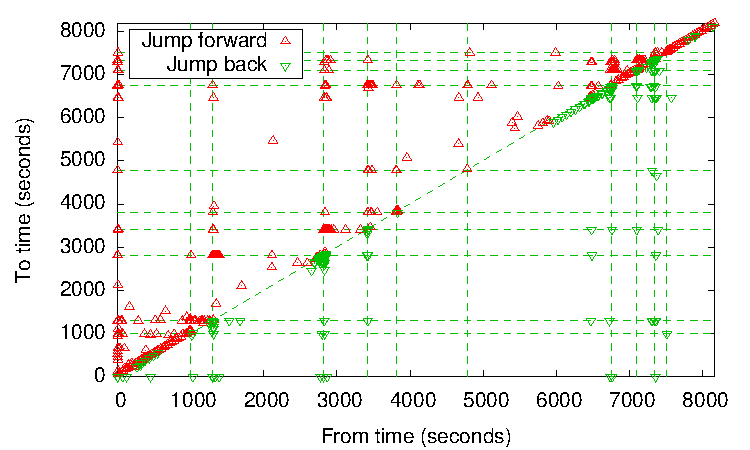
\includegraphics[width=0.5\columnwidth]{./graphs/arg-scg_jumps}
    }
    \subfloat[][Eurovision (cropped at 4000 seconds for clarity)] {
        \label{fig:eurovision_jumps}
        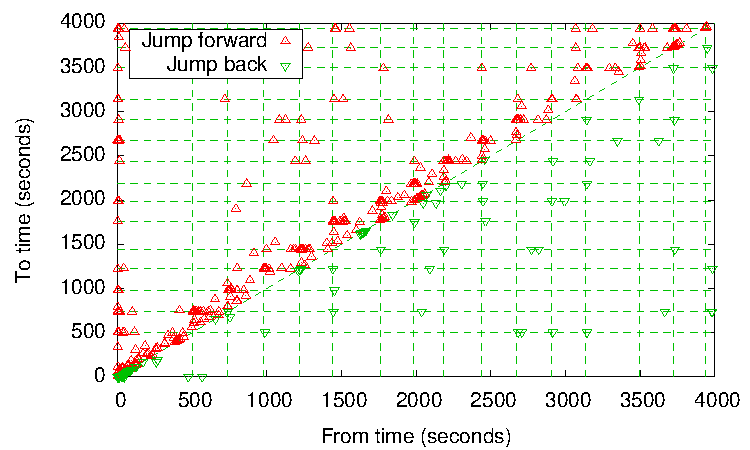
\includegraphics[width=0.5\columnwidth]{./graphs/eurovision_jumps}
    }

    \caption{Jumps made by users within two videos}
    \label{fig:jumps}
\end{figure}

To better understand how users navigated through a bookmarked video, we analysed the behaviour in the \emph{arg-scg} and \emph{eurovision} videos, which had 10 and 24 bookmarks respectively. In \autoref{fig:argscg_jumps} \& \autoref{fig:eurovision_jumps} each point is a seek that is identified by a ``from'' time on the x-axis and a ``to'' time on the y-axis. A point $x$,$y$ therefore represents a user that has jumped from their current playback point $x$ to a new point, $y$. Vertical and horizontal lines in the figures denote the position of the bookmarks. The diagonal line is a current-time marker such that seeks forward are points which lie above it, while seeks backward appear below it. Therefore, no point can fall precisely on the diagonal. It is immediately obvious from the figures that many points are on horizontal lines, implying that most seeks were to the bookmarks.

The forward seek buttons appear to have been mostly used for skipping to the next event, shown on both figures as points slightly above the diagonal line between the bookmarks. This could be due to user unfamiliarity with the bookmark interface, or possibly users simply browsing the video. Backward actions were typically used around bookmarks, where users would often re-watch the bookmarked event. In some cases users may also have wished to see video immediately preceding the bookmark. An example of this is shown in \autoref{fig:argscg_jumps} before the bookmark at time 2815, where users sought up to 75 seconds backwards to see more of the build up to the goal.

Clusters of points can also be seen on horizontal lines shortly after a vertical line, indicating that users jumped from bookmark to bookmark. In fact, the concentration of clusters of point just above the diagonal time reference indicates that users have a tendency to follow bookmarks in sequence, as exemplified in \autoref{fig:eurovision_jumps}.

Overall, for both videos these results demonstrate that users did not simply view continuously start-to-finish, and were in fact highly influenced when presented with bookmarks.

\section{Seek Distance}
\label{sect:seek_distance}

\begin{figure}[t]
    \centering

    \subfloat[][All seek distances] {
        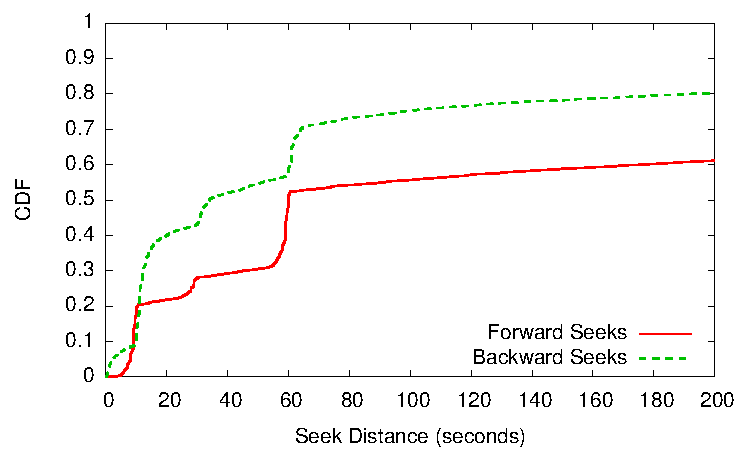
\includegraphics[width=0.5\columnwidth]{./graphs/all_jump_distance_200}
        \label{fig:seek_distance-a}
    }
    \subfloat[][All seeks cropped at 200 seconds] {
        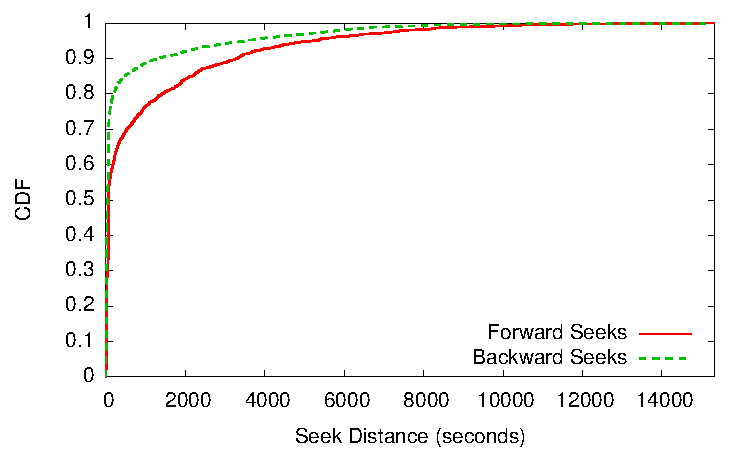
\includegraphics[width=0.5\columnwidth]{./graphs/all_jump_distance}
        \label{fig:seek_distance-b}
    }

    \caption{CDF of backward and forward seek distances}
    \label{fig:seek_distance}
\end{figure}

The understanding of locality is important for caching and pre-fetching algorithms. By looking at how far users sought we can determine the probability of accessing media nearby the playback point. We therefore define \emph{seek distance} as the absolute difference, in seconds, between a user's current playback point and their requested seek destination.

\autoref{fig:seek_distance-a} \& \autoref{fig:seek_distance-b} display a CDF of seek distance for backward and forward actions. A large proportion of seeks (between 50\%-70\%) are of a 15 seconds, 30 seconds, or 60 seconds values. These seeks represent the short seek button presses.
40\% of backward seeks were less than or equal to 15 seconds in length. This property could be exploited by keeping a small client side buffer of previously watched segments, which would satisfy many backward seeks if the user has already viewed them.
%The seeks do not occur exactly on their respective values because seeks can only be to a video keyframe, which were not always at exact second intervals.

% forwards mean 955.32
%  'Log-Normal'    'R_SQUARE ='    [0.96622]    'TEST ='    [58.528]    'MU ='[4.7599] 'SIGMA ='    [2.5265]
%  'Weibull'    'R_SQUARE ='    [0.94271]    'TEST ='    [96.206]    'l ='    [324.87] 'k ='    [0.42302]

% backwards mean 495.95
% 'Log-Normal'    'R_SQUARE ='    [0.96888]    'TEST ='    [21.927]    'MU ='    [3.6127] 'SIGMA ='    [1.7816]
% 'Weibull'    'R_SQUARE ='    [0.95186]    'TEST ='    [34.631]    'l ='    [69.156] 'k ='    [0.6563]

% forwards > 61 with mean 1968
% 'Log-Normal'    'R_SQUARE ='    [0.99259]    'TEST ='    [8.7149]    'MU ='    [6.8269] 'SIGMA ='    [1.5953]

% backwards > 61 with mean 1630
% 'Log-Normal'    'R_SQUARE ='    [0.98238]    'TEST ='    [4.5006]    'MU ='    [6.3273]  'SIGMA ='    [1.7906]

Even though small seeks are the majority, there are between 30\% and 50\% of seeks which are further than 60 seconds. These seeks consist of jumps to bookmarks or ``blind'' seeks with the seekbar. These long range seeks are log-normally distributed with a mean of 1968 seconds and 1630 seconds for forward and backward seeks respectively. They can be fitted to log-normal models with parameters $\mu = 6.8269$ and $\sigma = 1.5953$ for forward seeks, and $\mu = 6.3273$ and $\sigma = 1.7906$ for backward seeks. It can been seen that the backward distribution has a greater positive skew than the forward distribution, thus it will generate many small seeks.

%TODO add cool stat of how many of those 40\% rewinds could be satisified frmo a buffer

These behaviours exhibit a high degree of spatial locality, with the majority of seeks being within 60 seconds. Regarding long-ranged seeks, the log-normal distribution models imply that some very large distance seeks do occur, but the majority of seeks are shorter. Additionally, the skewed nature of this distribution is most likely because it is impossible to have a negative seek value. Overall the seek distances exhibit a median of 60 seconds for forward seeks and 34 seconds for backward seeks. This is consistent with previous findings~\cite{padhye1999cmc}.

%These behaviours exhibit a high degree of spatial locality, with the majority of seeks being within 60 seconds. Regarding long-ranged seeks, the log-normally distributed models imply that some very large distance seeks do occur, but the majority of seeks are shorter. Overall the seek distances exhibit a median of 60 seconds for forward seeks and 34 seconds for backward seeks. This is consistent with previous findings~\cite{padhye1999cmc}.

\section{Popularity}

\begin{figure}[t]
    % ploted with PlotPopularityRank()
    \centering
    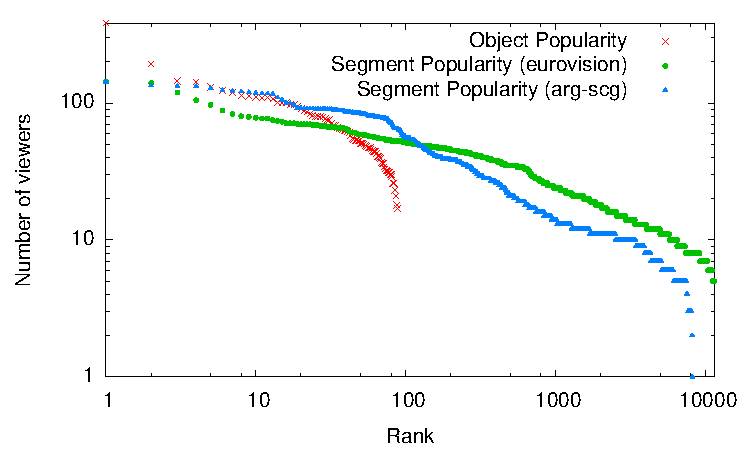
\includegraphics[width=0.5\columnwidth]{./graphs/all_sessions_rank}
    \caption{Object and segment popularity}
    \label{fig:popularity_object_rank}
\end{figure}

We study popularity in terms of the number of viewers who watched an \emph{object} or a \emph{segment}. An object in this system is a single video whereas a segment is a section of video one second in length.

The ranking for both object and segment popularity is shown in \autoref{fig:popularity_object_rank}. The \emph{eurovision}, and \emph{arg-scg} were approximately 10,000 seconds in length, causing \verb+~+10,000 segments to be ranked for each video. Recall that only 88 videos were available, so the lowest object rank is 88.

Typically object popularity with CDNs and VoD systems follows a power-law distribution~\cite{chesire2001maa,almeida2001aem,yu2006uub}, however, our analysis reveals otherwise. Instead the ranking of objects best fitted a normal distribution with parameters $\mu = 60$ and $\sigma = 32$. There are two reasons that power-law was not the best fit. Firstly, the catalogue of 88 videos was not very large, and secondly, power-law distributions do not fit well if the objects are constantly changing. Instead power-law fits better if a snapshot of rank \emph{vs.} popularity is taken each day and aggregated.

%Our analysis reveals that object popularity does not follow the typical power-law distribution observed within CDNs~\cite{chesire2001maa,almeida2001aem,yu2006uub} but instead is a normal distribution with parameters $\mu = 60$ and $\sigma = 32$. This can be attributed to the nature of our videos and the relatively few new objects each day.

% object pop (using rsqare)
%'Log-Normal'    'R_SQUARE ='    [0.99735]    'TEST ='    [0.015259]    'MU ='    [4.0391]    'SIGMA ='[0.55552]
%'Normal'    'R_SQUARE ='    [0.97996]    'TEST ='    [0.11636]    'MU ='    [60.129]    'SIGMA ='    [32.111]
%'Weibull'    'R_SQUARE ='    [0.99116]    'TEST ='    [0.050083]    'l ='    [70.549]    'k ='    [2.0227]

% object pop (using kst)
%'Log-Normal'    'R_SQUARE ='    [0.99708]    'TEST ='    [0.03116]    'MU ='    [4.03]    'SIGMA ='[0.55872]
% 'Normal'    'R_SQUARE ='    [0.97993]    'TEST ='    [0.077785]    'MU ='    [59.79]    'SIGMA ='    [30.131]
%'Weibull'    'R_SQUARE ='    [0.99039]    'TEST ='    [0.05571]    'l ='    [69.301]    'k ='    [2.114]


\begin{figure}[t]
    \centering

    %plotted with PlotViews()

    \subfloat[][Argentina vs. Serbia and Montenegro] {
        \label{fig:arg-scg_views}
        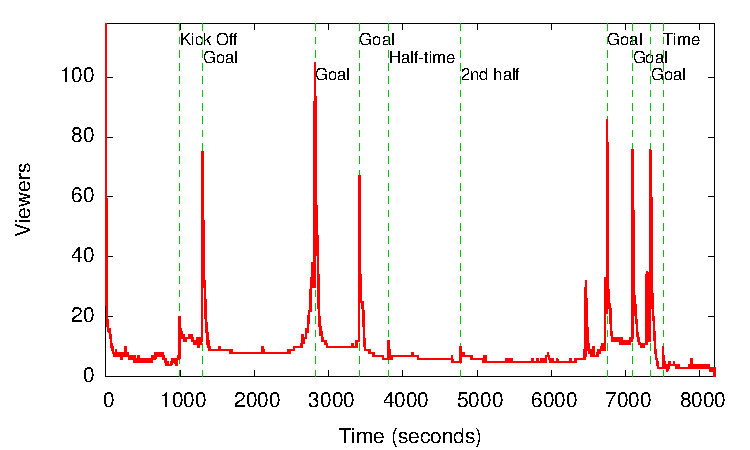
\includegraphics[width=0.5\columnwidth]{./graphs/arg-scg_views}
    }
    \subfloat[][Eurovision] {
        \label{fig:eurovision_views}
        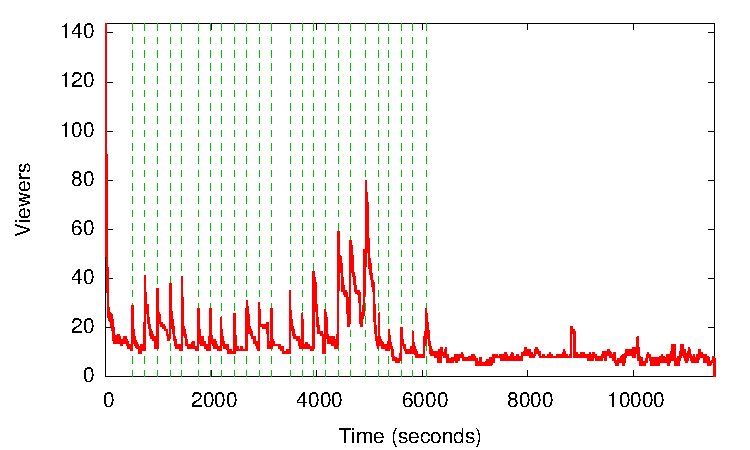
\includegraphics[width=0.5\columnwidth]{./graphs/eurovision_views}
    }

    \caption{Number of viewers at each second of video (each vertical line represents the position of a bookmark)}
\end{figure}

% euro (using rsquare)
%'Log-Normal'    'R_SQUARE ='    [0.99254]    'TEST ='    [0.035621]    'MU ='    [2.3233]    'SIGMA =' [0.56684]
%'Poisson'    'R_SQUARE ='    [0.95483]    'TEST ='    [0.24824]    'l ='    [11.142]
%'Weibull'    'R_SQUARE ='    [0.97982]    'TEST ='    [0.095445]    'l ='    [12.782]    'k ='    [1.8621]


% euro (using kst)
%'Log-Normal'    'R_SQUARE ='    [0.98993]    'TEST ='    [0.047187]    'MU ='    [2.3188]    'SIGMA ='    [0.49565]
%'Poisson'    'R_SQUARE ='    [0.95477]    'TEST ='    [0.14129]    'l ='    [11.132]
%'Weibull'    'R_SQUARE ='    [0.97678]    'TEST ='    [0.076196]    'l ='    [12.709]    'k ='    [2.3226]

% arg-scg (using rsqare)
%'Log-Normal'    'R_SQUARE ='    [0.99463]    'TEST ='    [0.03468]    'MU ='    [2.0063]    'SIGMA ='[0.58707]
%'Poisson'    'R_SQUARE ='    [0.98022]    'TEST ='    [0.13836]    'l ='    [8.5039]
% 'Weibull'    'R_SQUARE ='    [0.98978]    'TEST ='    [0.065082]    'l ='    [9.3509]    'k ='    [1.9405]

% arg-scg (using kst)
%'Log-Normal'    'R_SQUARE ='    [0.99428]    'TEST ='    [0.043658]    'MU ='    [2.0248]    'SIGMA ='[0.54523]
%'Poisson'    'R_SQUARE ='    [0.97926]    'TEST ='    [0.099252]    'l ='    [8.2927]
%'Weibull'    'R_SQUARE ='    [0.98943]    'TEST ='    [0.059218]    'l ='    [9.3725]    'k ='    [2.1449]

% all (using rsquare)
%'Weibull'    'R_SQUARE ='    [0.98284]    'TEST ='    [0.048803]    'l ='    [2.887]    'k ='    [0.69527]
%'Log-Normal'    'R_SQUARE ='    [0.98084]    'TEST ='    [0.054389]    'MU ='    [0.55114]    'SIGMA =' [1.3233]
%'Normal'    'R_SQUARE ='    [0.95011]    'TEST ='    [0.11357]    'MU ='    [2.5469]    'SIGMA ='    [3.4551]
%'Pareto'    'R_SQUARE ='    [0.94499]    'TEST ='    [0.13353]    'k ='    [0.97715]
%'Poisson'    'R_SQUARE ='    [0.92442]    'TEST ='    [0.2116]    'l ='    [2.923]
%'Zipf'    'R_SQUARE ='    [0.92855]    'TEST ='    [0.16903]    's ='    [1.7921]


% all (using kst)
%'Log-Normal'    'R_SQUARE ='    [0.965]    'TEST ='    [0.21597]    'MU ='    [0.95]    'SIGMA ='    [1.05]
%'Pareto'    'R_SQUARE ='    [0.94402]    'TEST ='    [0.21597]    'k ='    [1]
%'Normal'    'R_SQUARE ='    [0.93512]    'TEST ='    [0.13497]    'MU ='    [2.3933]    'SIGMA ='    [2.1693]
%'Zipf'    'R_SQUARE ='    [0.92861]    'TEST ='    [0.21597]    's ='    [1.79]
%'Poisson'    'R_SQUARE ='    [0.92163]    'TEST ='    [0.16872]    'l ='    [2.8265]

% Some matlab code to work out the top X %
% a = all_views(:,2);
% [y, x] = ecdf(a);
% x ( find(y > 0.99) ); limit = ans(1)
% sum( a ( find ( a > limit ) ) ) / sum( a )

% top 1% = 12% of requests
% top 10% = 44% of requests

%The popularity of one-second segments for all the videos exhibit a Weibull distribution with parameters $\lambda=2.887$
Again, the popularity of one-second segments might be best suited by a power-law, however Zipf and Pareto did not fit well. Instead, the popularity of one-second segments for all the videos exhibit a Weibull distribution with parameters $\lambda=2.887$ and $k=0.69527$. Log-normal distributions provide the best fits for the  \emph{arg-scg} and \emph{eurovision} results independently with parameters $\mu = 2.00, \sigma = 0.587$ and $\mu = 2.32, \sigma = 0.567$ respectively. Note that log-normal and Weibull distributions closely relate to power-law or heavy-tailed distributions~\cite{mitzenmacher2004abh,fishman2006hht}: they are skewed distributions where a small percentage of samples contributes to a sizeable weight of their distribution. We observe that a small percentage, (the 10\% most popular segments), accounted for about 44\% of all requests. Previously, Costa~\emph{et~al.}~\cite{costa2004aci} found that for educational and entertainment content, the popularity of segments is roughly uniformly distributed with a slight skew towards the beginning for entertainment content. Our result, however, implies that there are segments with orders of magnitude more viewers than others.

To illustrate the order-of-magnitude differences in viewers, we present \autoref{fig:arg-scg_views} \& \autoref{fig:eurovision_views} which show the popularity of each second of video for \emph{arg-scg} and \emph{eurovision} respectively. The vertical lines signify the position of the bookmarks; note for the \emph{eurovision} video there were no bookmarks after 6000 seconds as only the performances were bookmarked and they all appeared in the first half of the video. It is clear from the figures that there are peaks of popularity, highly influenced by the bookmarks. In \emph{arg-scg} (and in other sport content) we observe that most of the bookmarks are equally popular. However, in the \emph{eurovision} (and other music genres), we observe there is a greater variance in the popularity of the bookmarks. This can be attributed to sports having numerous events which all users wish to watch, however in music videos there may be only certain artists which interest the user.

Popularity metrics are important to many CDN algorithms as they help to decide which resources to allocate to each object. We have seen that bookmarks within videos cause segments to be of high interest and popularity, for example, goals within a sporting event. This result emphasises the use of partial caching techniques~\cite{chen2003aal} to cache only popular segments.

\section{Longevity}
\label{sect:stay_popular}

\begin{figure}[t]
    % plotted with PlotPopularityLifetime()
    \centering
    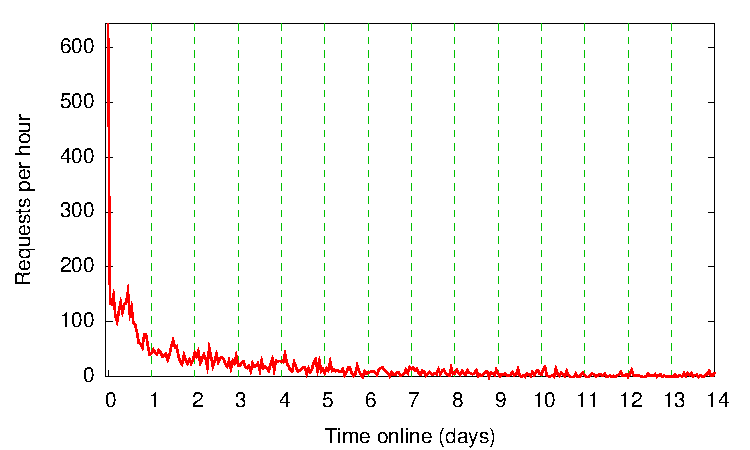
\includegraphics[width=0.5\columnwidth]{./graphs/all_bookpop_lifetime}
    \caption{Bookmark utilisation within all videos over time, following initial usage}
    \label{fig:lifetimes}
\end{figure}

%    'Weibull'    'R_SQUARE ='    [0.99796]    'TEST ='    [0.042635]    'l ='    [3.1004]    'k ='    [0.61592]
%    'Log-Normal'    'R_SQUARE ='    [0.98626]    'TEST ='    [0.28989]    'MU ='    [0.52115]    'SIGMA ='    [1.5475]

The popularity of both videos and bookmarks in our system changed over time. This phenomenon is outlined in \autoref{sect:pop_over_time} which describes how and why the popularity changes. However, in our results the popularity always declined, therefore we call the duration at which any such item remains utilised its \emph{longevity}. The study of a video or bookmark's longevity can aid cache replacement policies, as well as other content management decisions.

\autoref{fig:lifetimes} shows the popularity of all our bookmarks versus the time they were first used. The figure suggests that following an initial peak and a slight resurgence, there was a rapid decrease in interest after a short period. R-Square fitting reveals that the bookmark longevity can be suitably estimated using a Weibull distribution with $\lambda=3.10$ and $k=0.615$. This suggests that the popularity exhibits long-tailed properties. We also observe that 40\% of the bookmark usage occurs within 24 hours, with the remainder slowly occurring over the following weeks. This is in line with the previous research on this topic~\cite{cherkasova2004aoe}.

The popularity of videos decreased over time, but this is not true for the popularity of segments within the videos. For example, the segments which were popular within that video when it was first published were still popular within the video weeks later, long after the video had lost it overall popularity. This was tested on each video by calculating the distribution of segment popularity for the first 50\% of requests versus the last 50\% of requests. The difference in distributions was minor, with an average R-Square value of 0.9. On a visual inspection of the number of viewers per second, it was clear that the popularity still focused around the bookmarks.

\section{Session Lengths}

\begin{figure}[t]
    \centering
    %plotted with PlotSessions()

%    \subfigure[All videos] {
%        \label{fig:view_user_session}
%        \includegraphics[width=0.5\textwidth]{./graphs/all_user_sessions}
%    }
    \subfloat[][Eurovision] {
        \label{fig:eurovision_user_session}
        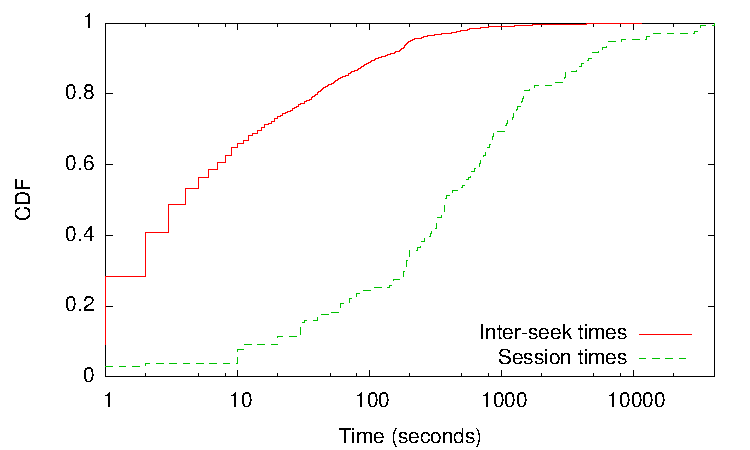
\includegraphics[width=0.5\columnwidth]{./graphs/eurovision_user_sessions}
    }
    \subfloat[][Argentina vs. Serbia and Montenegro] {
        \label{fig:arg-scg_user_sessions}
        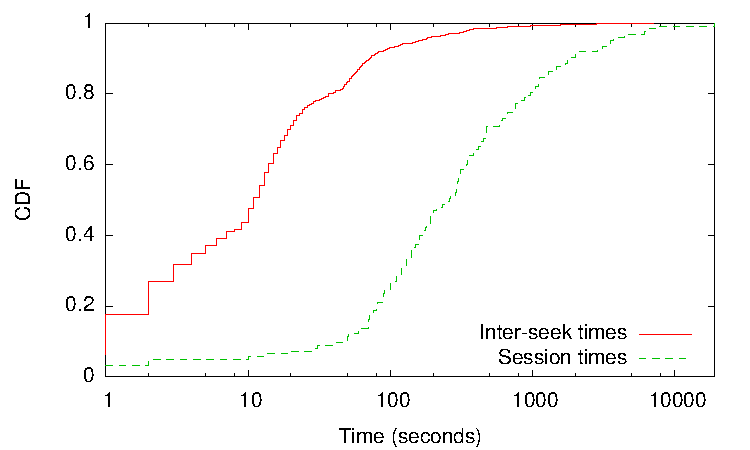
\includegraphics[width=0.5\columnwidth]{./graphs/arg-scg_user_sessions}
    }

    \caption{CDFs of session lengths and inter-seek times}
    \label{fig:view_user_sessions}
\end{figure}

Session length is the total time a user accessed a video, regardless of the actions they may have taken whilst doing so. For example, a session may be longer than the actual length of the video if the user chose to re-watch segments, and/or pause.

\autoref{fig:eurovision_user_session} \& \autoref{fig:arg-scg_user_sessions} show the CDF of both session and inter-seek times (discussion of inter-seek times follows in the next subsection). It can be observed from the session times that most users access each video for a very short time relative to its overall length (possibly just watching the events they are interested in). In particular, note that in the \emph{arg-scg} case around 80\% of sessions lasted less than 15 minutes. Given that the video was 2.2 hours in length, 15 minutes corresponds to only 11\% of the total video. A similar result was found with \emph{eurovision}, with 80\% of sessions lasting less than 12\% of the total video duration. The average session duration was found to be only 11 minutes and 18 minutes for \emph{arg-scg} and \emph{eurovision} respectively.

We also found that a small minority (roughly 3\%) of session durations were longer than the length of a video. Of these durations roughly 39\% were between 3 to 8 hours long. Our logs show that these users paused for a long time before deciding to resume playback.

%These outliers are possibly why we observe that session sizes are best fitted by a log-normal distribution with parameters $\mu=4.73$ and $\sigma=1.90$.

%    'Log-Normal'    'R_SQUARE ='    [0.99779]    'TEST ='    [0.1091]    'MU ='    [4.7315]    'SIGMA ='[1.9014]
%    'Normal'    'R_SQUARE ='    [0.86057]    'TEST ='    [7.3338]    'MU ='    [143.77]    'SIGMA ='    [489.46]
%    'Weibull'    'R_SQUARE ='    [0.98666]    'TEST ='    [0.65005]    'l ='    [233.17]    'k ='    [0.51125]

\section{Inter-seek Times}
\label{sect:interseek}

Inter-seek time is described as the duration for which a user watched a section of a video before seeking to a new location (disregarding any paused periods). This can be useful, for example, to determine the amount to replicate when using partial caching.

From our logs, we found that on average a user performed 8.98 seek operations around a video, resulting in a mean inter-seek time of 50.4 seconds. \autoref{fig:eurovision_user_session} \& \autoref{fig:arg-scg_user_sessions} show the CDF for inter-seek times as well as session length. As the inter-seek times are generally shorter than session times, this implies that the majority of users viewed the content as a series of excerpts, usually under a minute in length.

%It can been seen that around 50\% of viewed sections of videos were
%less than 8 seconds in length, and around 80\% of users watched the
%video for less than 50 seconds before seeking again. Less than 1\%
%of all users watched more than 1000 seconds of consecutive video.


%'Log-Normal'    'R_SQUARE ='    [0.99644]    'TEST ='    [0.020535]    'MU ='    [1.2886]    'SIGMA ='    [2.318]
%'Zipf'    'R_SQUARE ='    [0.91125]    'TEST ='    [0.36561]    's ='    [1.483]
%'Pareto'    'R_SQUARE ='    [0.92868]    'TEST ='    [0.30414]    'k ='    [0.57246]
%'Weibull'    'R_SQUARE ='    [0.99353]    'TEST ='    [0.037535]    'l ='    [7.5243]    'k ='    [0.35646]


The inter-seek time in the music content was found to be on average longer. This is because the length of a bookmarked musical performance generally exceeds the length of an event within a football match. Regardless of the difference in inter-seek times, we found that they can be estimated by log-normal distributions. For instance, the inter-seek time for \emph{arg-scg} can be modelled with parameters $\mu=2.15$ and $\sigma=1.72$.

Previous studies have found that the majority of inter-seek times are very short~\cite{vilas2005uba}. For long educational content, inter-seek times have also been shown to be Weibull distributed or a combination of Weibull for
the body and Pareto for the tail~\cite{almeida2001aem}. We found that most of our videos had inter-seek times that could be suitably modelled by a Weibull distribution, and two thirds which could be modelled with Pareto alone. Models of inter-seek times can be used by a delivery system to determine the size of video replicas and the time available to react before a user seeks elsewhere in the video.

\section{Sequence}
\label{sect:sequence}

% TODO Place both figures next to each other
\begin{figure}[t]
    \centering
    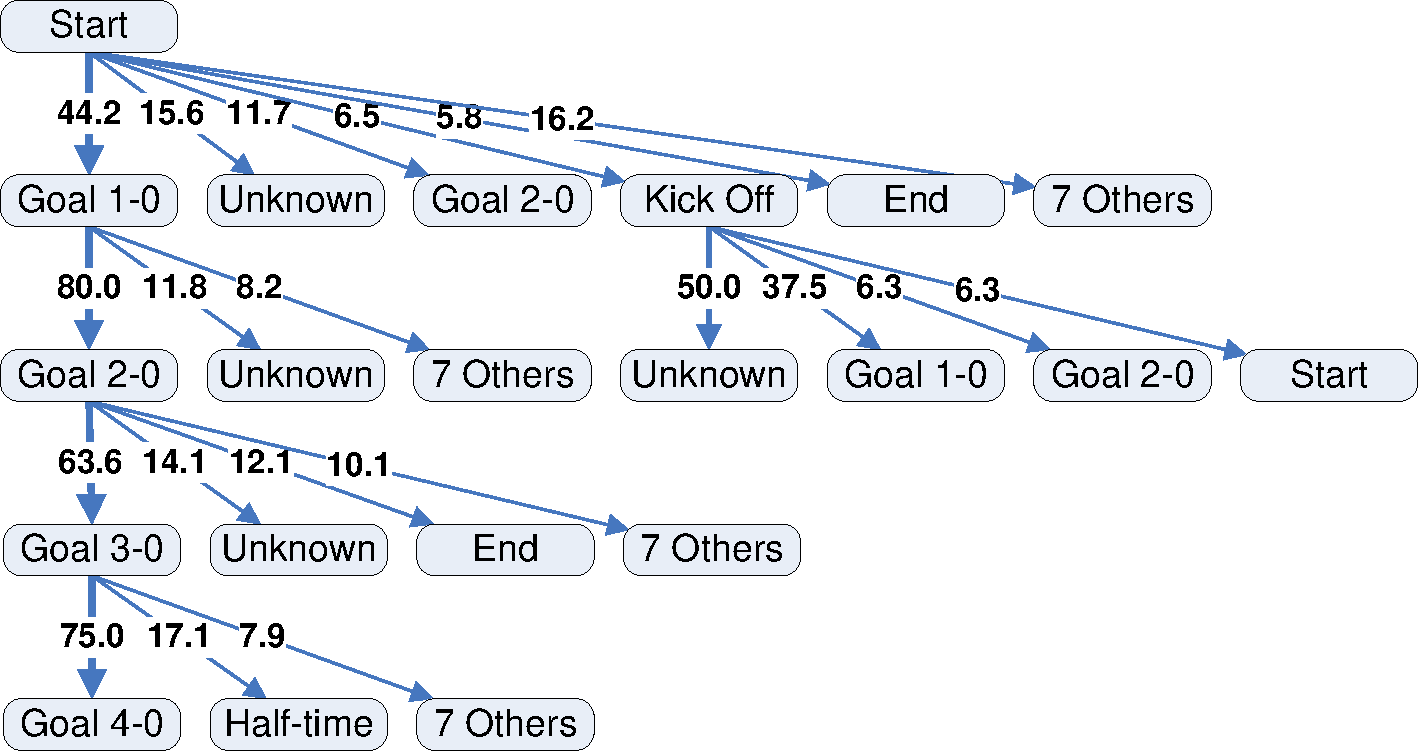
\includegraphics[width=0.50\columnwidth]{./diagrams/sequence}
    \caption{Sequence diagram for Argentina vs. Serbia and Montenegro depicted as a tree}
    \label{fig:sequences}
\end{figure}

\begin{figure}[t]
    %plotted with PlotSequence()
    \centering
    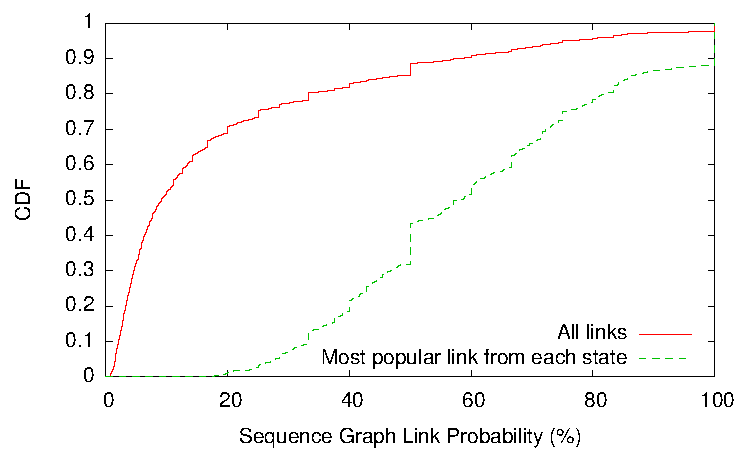
\includegraphics[width=0.50\columnwidth]{./graphs/all_sequence_normal_cdf}
    \caption{CDF of link probabilities for all videos}
    \label{fig:all_sequence}
\end{figure}

The traces were analysed to study the extent to which users' actions could be predicted. Since jumps to bookmarks made up a relatively large percentage of all requests, we limit this prediction to which bookmark will be visited next.
If a system could predict which bookmark would be requested next by a user, then it could pro-actively respond in order to optimise content delivery. For example, based on the next predicted bookmark, the relevant segments could be pushed out by a server with spare capacity, or pre-fetched by a client.

% 200seconds is longer than 96% of all interseek times
We call the order that bookmarks are viewed by a single user a {\em sequence} of bookmarks. Every user's sequence can be aggregated together to form a directed graph. Each node in the graph represents a bookmark with links between them representing the probability of seeking to that bookmark next. \autoref{fig:sequences} shows a section of one of these directed graphs depicted as a tree for clarity. The ``Start'' node represents the beginning of the video, and the ``End'' node represents the completion of a session. There is also an ``Unknown'' node which signifies when a seek to another bookmark has not been made within 200 seconds of visiting the previous bookmark (the observed upper bound for bookmarked events' length). For clarity, links with low probabilities have also been aggregated to form a ``$N$ Others'' node, where $N$ is the number of aggregated links.

It is clear from the figure that there are multiple choices to visit from each node, although there is generally one link that is significantly more likely to be chosen. For example, the probability of viewing bookmark ``Goal 2-0'' immediately after ``Goal 1-0'' is 80\%. We can also see that following the ``Kick Off'' bookmark 50\% of users did not visit another bookmark within 200 seconds and instead continue to watch, this could indicate that this subset of users were interested in watching the full game instead of just the highlights. An interesting observation for caching is the occurrence of self-loops. 6\% of links were between the same two bookmarks, which made up 6.5\% of all requests.

To understand how many bookmark-to-bookmark links are predictable, \autoref{fig:all_sequence} shows a CDF of probabilities for all links for all videos, as well as probabilities for just the most popular link from each bookmark. From this figure we can conclude that 10\% of all links have more than a 58\% chance of being followed.
Looking at just the most popular link from each bookmark we observe that over half of the bookmarks have an outgoing link with a probability over 50\%; an encouraging result for user predictability.

In this analysis we assumed that all users will visit the bookmark in similar order, however in a large heterogeneous environment this may not be true. Different sub-groups may wish to view a different set of events possibly in a different order to other sub-groups. Across our videos we did try and identify if there were groups of individuals that behaved differently to the majority, however none were found. This could possibly be due to our genre of media, with all sports fans wishing to see the same events, in the natural sequential order.

%Fig.~\ref{fig:all_sequence} shows that around the top 20\% of bookmark sequence pairs were followed by more than 50\% of users. This means that there is a high chance of predicting these bookmark sequences. Note that these bookmarks also consist of the 20\% most popular bookmarks. However, the figure also shows that it is generally difficult to predict the actions of a user if all actions are considered. This is because of the wider range of interactivity options a user has when VCR functionality is also considered.

%The exact parameters are of little importance, however the type of distribution used implies the impact on the system.

%Observe that
%the {\em log-normal} distribution emerges as the best model for most
%of the observed features in our experiment, except for object
%popularity and arrival rates, which are best modelled by {\em Normal
%} and {\em Weibull} distributions respectively. This is unsurprising
%because log-normal distributions are commonly known to model various
%properties in computing systems. Weibull and, as noted earlier,
%log-normal distributions both closely relate to power-law or
%heavy-tailed distributions~\cite{geor06}.

\begin{figure}[t]
    \centering

    % Plotted with PlotBookmarkWaitsMerge

    \subfloat[][Argentina vs. Serbia and Montenegro] {
        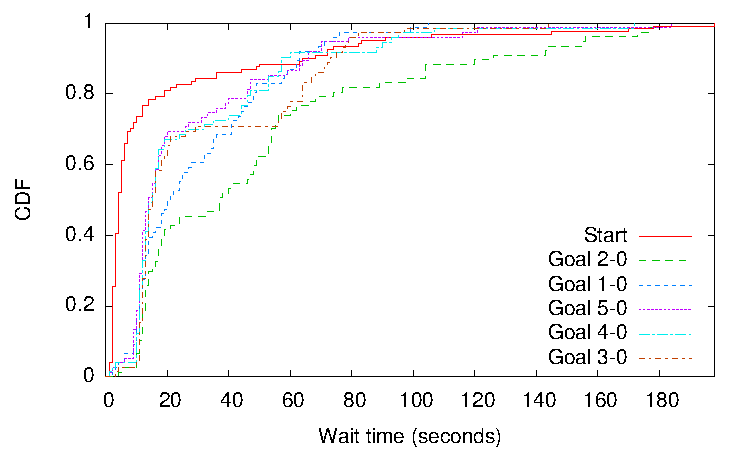
\includegraphics[width=0.5\columnwidth]{./graphs/arg-scg_all_waitjumps}
        \label{fig:waitjumps-a}
    }
    \subfloat[][Eurovision] {
        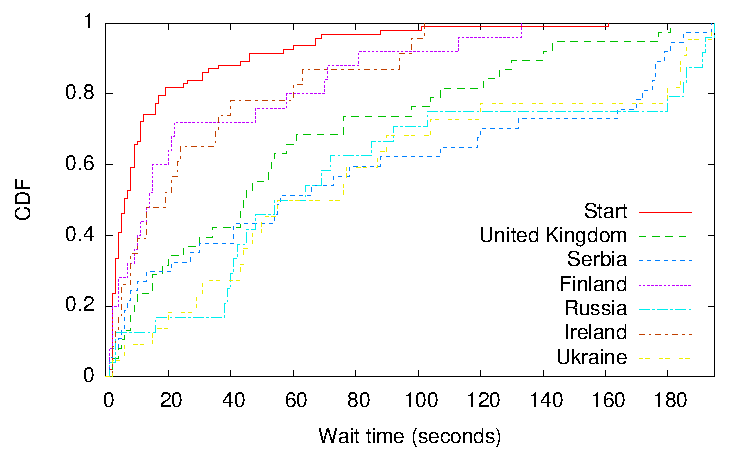
\includegraphics[width=0.5\columnwidth]{./graphs/eurovision_all_waitjumps}
        \label{fig:waitjumps-b}
    }

    \caption{CDFs of wait times}
    \label{fig:waitjumps}
\end{figure}

\section{Hotspot Length}
\label{sect:hotspot_length}

Jumps to bookmarks comprised roughly 20\% of all requests with an additional 32\% of seeks being within 60 seconds of a bookmark. Bookmarks form the majority of requests within the content, and represent the beginning of a popular segment of video which we call a \emph{hotspot}. The beginning of a hotspot is generally known (\emph{i.e.}, the bookmark point), but the end is not. Knowing the length of the hotspot can be useful for numerous tasks such as caching and pre-fetching. We therefore define \emph{wait time} as the time elapsed between a user following a bookmark and seeking.

\autoref{fig:waitjumps-a} \& \autoref{fig:waitjumps-b} show a CDF of wait times for each bookmark in the \emph{arg-scg} and \emph{eurovision} videos. It can be seen that in the football match the wait times follow a similar distribution, with the majority of users waiting less than 40 seconds (this, for example, could corresponds to the length of a run up to a goal). The \emph{eurovision} results are more varied with average wait times being much longer. This is due to the typical song in the Eurovision Song Contest being 180 seconds in length.  Finally, there is a ``Start'' bookmark listed in both figures: this is the entry point into both videos, and does not correspond to any event.

To better understand the wait times, distributions were fitted. In the general aggregated case a Weibull model fits best with parameters $\lambda=24.594$ and $k=0.7034$. For individual bookmarks log-normal and Weibull models proved best in the majority of cases.
%This result is similar to the inter-seek times in Section~\ref{sect:interseek}.
With these models the upper bound of a hotspots' lengths can be extrapolated by using, for example, the 95\sth percentile.

%'Log-Normal'    'R_SQUARE ='    [0.98463]    'TEST ='    [0.1127]    'MU ='    [2.6361]    'SIGMA ='    [1.388]
%'Weibull'    'R_SQUARE ='    [0.99545]    'TEST ='    [0.033063]    'l ='    [24.594]    'k ='    [0.7034]
%'Zipf'    'R_SQUARE ='    [0.93259]    'TEST ='    [0.34879]    's ='    [1.018]

\section{User Behaviour Models}

\begin{table}[tbp]
    \centering{\small
    \begin{tabular}{|rcc|}
      \hline
\setrowcolor{TableRowHead}
      Metric & Distribution & R-square \\
      \hline
\setrowcolor{TableRowA}
      Object Popularity  & Normal ( $\mu=60.129$ , $\sigma=32.111$ )     & 0.97996 \\
\setrowcolor{TableRowB}
      Segment Popularity & Log-normal ( $\mu=0.551$ , $\sigma=1.32$ )   & 0.98084 \\
\setrowcolor{TableRowB}
                         & Weibull    ( $\lambda=2.887$ , $k=0.69527$ ) & 0.98284 \\
\setrowcolor{TableRowA}
      Session Length     & Log-normal ( $\mu=4.73$, $\sigma=1.90$ )     & 0.99779  \\
\setrowcolor{TableRowA}
                         & Weibull    ( $\lambda=233.17$, $k=0.51125$ ) & 0.98666 \\
\setrowcolor{TableRowB}
      Inter-seek times   & Log-normal ( $\mu=1.2886$, $\sigma=2.318$ )  & 0.99644 \\
\setrowcolor{TableRowB}
                         & Weibull    ( $\lambda=7.5243$, $k=0.35646$ ) & 0.99353 \\
\setrowcolor{TableRowA}
      Seek Distance (forward)      & Log-normal ( $\mu = 7.2668$, $\sigma = 1.2194$ )  & 0.99567 \\
      \setrowcolor{TableRowB}
      Seek Distance (backward)     & Log-normal ( $\mu = 7.195$, $\sigma = 1.3132$ )   & 0.99083 \\
\setrowcolor{TableRowA}
      Hotspot Length    & Log-normal ( $\mu=2.6361$, $\sigma=1.388$ )  & 0.98463 \\
\setrowcolor{TableRowA}
                         & Weibull    ( $\lambda=24.594$ , $k=0.7034$ ) & 0.99545 \\
\setrowcolor{TableRowB}
      Bookmark Longevity & Weibull    ( $\lambda=3.1004$ , $k=0.61592$ ) & 0.99796 \\
    \hline
    \end{tabular}
    }
    \caption{A summary of metrics with their corresponding distributions}
    \label{tab:models}
\end{table}

Model fitting is important for understanding the different properties of the system, and aids in simulation creation and algorithmic design. Various models have been discussed for the different parameters of the system. In all cases many models (\emph{e.g.}, normal, log-normal, exponential, Weibull, Pareto, Poisson, Zipf) were fitted to the data with varying success. Generally, more than one distribution fitted well. This subsection will summarise the analytical models found for each parameter.

\autoref{tab:models} gives an overview of the best matching models for each metric discussed previously, with their corresponding \emph{R-square} values. Of particular importance are the types of distribution which can have a significant impact on the system. For example, the Weibull and log-normal models are both long-tailed, and systems may have to anticipate the skewed distribution to cope effectively.

%\begin{table}[tb]
%    \centering\scriptsize
%
%    \begin{tabular}{|ccccccccc|}
%      \hline
%\setrowcolor{TableRowHead}
%      Metric & Max Models & Log-normal & Weibull & Pareto & Normal & Exponential & Zipf & No fit\\
%      \hline
%\setrowcolor{TableRowA}
%      Segment Popularity & 84 (from 88 videos) & 61  & 65  & 12 & 58 & 42 & 13 & 17\\
%\setrowcolor{TableRowB}
%      Session Length     & 81 (from 88 videos) & 75  & 72  & 0  & 5  & 31 & 4  & 0\\
%\setrowcolor{TableRowA}
%      Inter-seek times   & 87 (from 88 videos) & 83  & 83  & 54 & 1  &  3 & 55 & 3\\
%\setrowcolor{TableRowB}
%      Hotspot Length    & 203 (from 695 bookmarks) & 165 & 135 & 91 & 5  & 48 & 53 & 22 \\
%      \hline
%    \end{tabular}
%    \caption{Metrics for individual videos and their corresponding distributions}
%    \label{tab:models_all}
%\end{table}
%
%The models shown so far are from aggregated results across all the videos. Instead, it may be interesting to model the different metrics of each particular video. However due to the diversity in models and parameters it is not possible to show each model, so instead \autoref{tab:models_all} summaries which models fit with a \emph{R-square} value greater than 95\%. The ``max models'' column represents the number of datasets that are of sufficient size to have models fitted. For example, there are 695 bookmarks, yet only 203 had enough data to be fitted to a hotspot length, and of these, 165 fitted well to a Log-normal model, 135 to a Weibull models, \emph{etc}.

\section{Summary}

%In this section we have shown:
%    When presented with bookmarks users are highly influences by them
%    This causes the popularity of seconds to be heavy-tailed
%    Session times are very short compared to media
%    A sequence of bookmarks can be predicted
%
%    Can we make sure bookmarks help the system as much as possible?
%    Can we predict which bookmark is next?

Our results have shown that the interactivity options available to users highly influence their behaviour. In particular, it was found that the novel interactive feature of \emph{bookmarking} played a pivotal role, leading to access patterns quite dissimilar from previous related studies that looked at VCR-like interactivity alone.
The combination of our content type and the addition of bookmarks led to users accessing content in relatively short segments sparsely distributed throughout the length of the videos. Segment popularity is skewed with the most popular segments clearly around the bookmarks, forming hotspots. From both a user and a content distribution network's perspective, this can be viewed as advantageous; users can reach interesting content more quickly through the bookmarks, and the increased locality of interest means CDNs can respond more effectively by, for example, prioritising hotspot replication.

Content placement is an important and difficult problem for CDNs. The CDN has to decide where within the network to replicate or cache content. Typically the content is placed near to the users, and replicated as a whole. However, as we have seen, not all segments within a piece of content are equal and a CDN can leverage this information to replicate certain segments more than others. This is especially useful when popularity nearly always concentrates around bookmarks, allowing the relevant segments to be replicated throughout the network before user demand increases.

A CDN could be designed to handle high levels of user interactivity, with relatively short sessions and inter-seek times. Our results have shown that hotspots following bookmarks were orders of magnitude shorter than the video containing them. Furthermore, it encourages the use of an agile delivery mechanism that allows distribution of small sparsely distributed segments quickly and efficiently.

We have also shown that users view the bookmarks in a similar order, giving them a degree of predictability. This could allow a CDN to exploit pre-fetching techniques to improve the user's experience. For example, if the CDN could predict the next segment the user will watch, then this could be pre-fetched into the user's playback buffer and when the user seeks to that segment there will be no delay caused by seek latency and buffering.

The use of bookmarks depends on them being well positioned and of interest to the user. We noted in the first experiment that 40\% of bookmarks had at least one user seek before the bookmark, with 30.7\% of these seeks occurring within 5 seconds of jumping to the bookmark. This perhaps represents users who were almost immediately dissatisfied with the bookmark's location. We noted this happened consistently for roughly 6\% of the total bookmarks. Upon further inspection, it appeared the bookmarks were inadvertently misplaced. This led to users performing additional seeks to find the correct location, thus placing extra load on the servers.

% CHECKME
Throughout the experiment different genres of videos were available to the users, namely sporting and musical videos. Only the analysis of the ``Argentina vs. Serbia and Montenegro'' football match and the ``Eurovision song contest'' were shown in this chapter, however other sporting events were available on the site such as Formula~1 racing, International Cricket, and other miscellaneous recordings of music channels. Similar patterns were observed for each video, however, semantics of the content did have some impact of how the users consumed the data.

All videos exhibited similar patterns, for example, popularity was generally centered around the bookmarked segments, and that the viewing duration was far shorter than the full length of the video. However, minor differences were found, for example, the music channels had greater variance in the popularity of each bookmark (which were placed at the beginning of individual music videos). This can easily be attributed to users only being interested in particular artists or videos, whereas viewers of sporting events would be interested in every highlight (and therefore every bookmark). Similar differences were found in the inter-seek times, session times, and hotspot lengths, as the semantics of the content would determine how long particular hotspots were. However, metrics such as the number of interactions, or bookmark longevity stayed the same, as these did not appear to be directly impacted by the content.

In the following chapter, we explore and study the implications of a few techniques designed to exploit some of the properties suggested from our analysis. The first addresses the dynamic re-positioning of bookmarks in response to user behaviour. The second concerns predictive pre-fetching of popular segments to enhance the efficiency of delivery of highly interactive content. The last technique is an evaluation of how well existing delivery mechanisms behaviour when delivering interactive media, and how this can be improved with an hybrid approach.

    \chapter{Techniques for Interactivity Support}
\label{chap:new_techiques}

%\todo{Where is the hotspot detection stuff?}

% simple dynamic bookmark placement and interactivity-aware content pre-fetching and replication

So far, this thesis has outlined a twelve month experiment in which highly interactive user behaviour was recorded. The traces obtained from the experiment have been analysed and characterised to produce a set of models and user workloads. These workloads and models were developed so future ideas and concepts could be designed and tested with realistic data.

This chapter outlines some of the improvements which can be made to aid in the delivery of this genre of content. This includes a system to dynamically position bookmarks within the media, a way to pre-fetch segments of the media ahead of their request, and an evaluation of hybrid delivery technique designed to deliver highly interactive content.

\section{Dynamic Placement of Bookmarks}
\label{sect:moving_bookmark}

During our experiments, bookmarks were appropriately positioned by administrators before the video was published. It was previously noted that a small percentage of bookmarks (roughly 6\%) were unintentionally misplaced. There are many reasons why a bookmark could be misplaced, such as human error, or a lack of insight into user requirements. For example: a bookmark could be placed before a penalty kick, but many users may first wish to see the foul that led to the penalty. As such, it would be beneficial if the system could autonomically detect poorly placed bookmarks and correct them based on automatic feedback derived from the user's actions.

During the second video trial, we took the opportunity to go beyond characterising user behaviour, by testing a dynamic bookmark placement technique in the live system. This technique inferred if the bookmark was misplaced based on the user's seeking behaviour, and then correct the bookmark's position in a reactive way. The remainder of this section discusses and analyse this technique.

%For example a football goal bookmark would be placed at the position the scoring team gained possession of the ball just before the goal. This allowed the user to view the run up to the goal, as well as the goal itself.


\begin{figure}[t]
    \centering

%    %http://www.ctan.org/tex-archive/graphics/pgf/doc/generic/pgf/version-for-pdftex/en/pgfmanual.pdf
\begin{tikzpicture}[scale=2.3]

    \node[right] at (-1.5, 0.85) {\textbf{Scenario A}};

    \draw [|->] (-1.5,0) -- (2,0);
    \draw (0, 0) -- (0,0.125);

    \node (start) at (0,-0.3)  {};
    \node (bookmark) at (0,0)  {};
    \node (wait) at (1,0) {};
    \node (jump) at (-1,0) {};

    \begin{scope}[>=latex, very thick]
        \draw [->] (start.north) -- node[left] {1. Jumps to $B_{t}$} (bookmark.south);
        \draw [->] (bookmark.north) -- node[near end, below=3pt] {2. Watches for $w$} (wait.north);
        \draw [<-] (jump.north) .. controls +(up:0.4) and +(up:0.4) .. node[above] {
            3. Seeks to $S_{t}$ ($S_{t} < B_{t}$)
        } (wait.north);
    \end{scope}

    %\draw [|-|, dotted] (bookmark.south) -- node[below] {$d$} (jump.south);

\end{tikzpicture}

\begin{tikzpicture}[scale=2.3]

    \node[right] at (-1.5, 0.7) {\textbf{Scenario B}};

    \draw [|->] (-1.5,0) -- (2,0);
    \draw (0, 0) -- (0,0.125);

    \node (start) at (0,-0.3)  {};
    \node (bookmark) at (0,0)  {};
    \node (wait) at (1,0) {};
    \node (jump) at (0.25,0) {};

    \begin{scope}[>=latex, very thick]
        \draw [->] (start.north) -- node[left] {1. Jumps to $B_{t}$} (bookmark.south);
        \draw [->] (bookmark.north) -- node[near end, below=3pt] {2. Watches for $w$} (wait.north);
        \draw [<-] (jump.north) .. controls +(up:0.25) and +(up:0.25) .. node[above] {
            3. Seeks to $S_{t}$ ($B_{t} < S_{t} < B_{t} + w$)
        } (wait.north);
    \end{scope}

    %\draw [|-|, dotted] (bookmark.south) -- node[below] {$d$} (jump.south);

\end{tikzpicture}

\begin{tikzpicture}[scale=2.3]

    \node[right] at (-1.5, 0.7) {\textbf{Scenario C}};

    \draw [|->] (-1.5,0) -- (2,0);
    \draw (0, 0) -- (0,0.125);

    \node (start) at (0,-0.3)  {};
    \node (bookmark) at (0,0)  {};
    \node (wait) at (1,0) {};
    \node (jump) at (1.75,0) {};

%TODO If have time maybe fix point 3 to be cantered better

    \begin{scope}[>=latex, very thick]
        \draw [->] (start.north) -- node[left] {1. Jumps to $B_{t}$} (bookmark.south);
        \draw [->] (bookmark.north) -- node[near end, below=3pt] {2. Watches for $w$} (wait.north);
        \draw [<-] (jump.north) .. controls +(up:0.25) and +(up:0.25) .. node[above left=12pt, pos=0] {
            3. Seeks to $S_{t}$ ($S_{t} > B_{t} + w$)
        } (wait.north);
    \end{scope}

    %\draw [|-|, dotted] (bookmark.south) -- node[below] {$d$} (jump.south);

\end{tikzpicture} 
    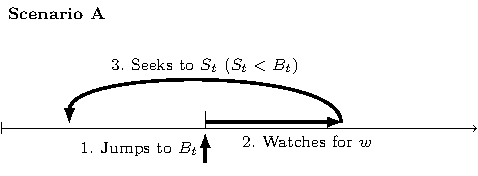
\includegraphics[width=0.7\columnwidth]{./diagrams/scenarios_A}
    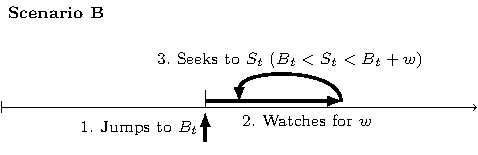
\includegraphics[width=0.7\columnwidth]{./diagrams/scenarios_B}
    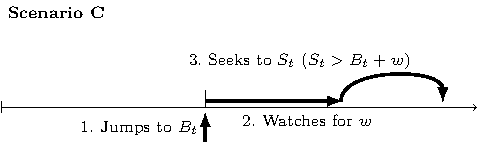
\includegraphics[width=0.7\columnwidth]{./diagrams/scenarios_C}

    \caption{Different scenarios that may induce bookmark movement}
    \label{fig:movingbookmark}
\end{figure}

To develop a reactive algorithm that moves bookmarks dependent on user behaviour, different possible scenarios should first be explained. \autoref{fig:movingbookmark} shows three different sequences of actions a user could follow shortly after seeking to a bookmark.

\begin{description}
  \item[Scenario A] shows the user briefly viewing the bookmark, then seeking to a time earlier than it. While this could indicate that the bookmarked event was short and that the user wanted to view it again, it could equally imply that the bookmark was placed later than it should have been.
  \item[Scenario B] is similar to \emph{Scenario A} but differs in that the user does not seek back to a point before the bookmark; this means the user is simply replaying footage, thus implying the bookmark is correctly placed for that individual.
  \item[Scenario C] represents a situation in which the user's motives are difficult to determine. Since they watch briefly then seek forward, several possibilities exist: the bookmarked event may have ended, the bookmark may have been placed prematurely, or the user is simply seeking forward towards the next event.
\end{description}

A further possibility, not shown in the figure, is for a user to seek far away from a bookmark in either direction. Since it is unlikely their destination would be related to the bookmark, such an action would not indicate the bookmark was incorrectly placed.

\emph{Scenario A} and \emph{Scenario C} are therefore the only scenarios where the user's actions could indicate the bookmark is misplaced. All other actions should reinforce the position of the bookmark to reduce future movements once it is correctly placed. Additionally since we are less sure of the user's intentions in \emph{Scenario C} we should only make minor changes to the bookmark's placement to limit the impact of false-positives.

\renewcommand{\algorithmiccomment}[1]{// #1}
\begin{algorithm}[t]
{\small
\begin{algorithmic}[0]
    \STATE\COMMENT{$B_{t}$ is the location of the bookmark at time $t$}
    \STATE\COMMENT{$S_{t}$ is the location the user sought at time $t$}
    \STATE\COMMENT{$w$ is the time the user waited before seeking to $S_{t}$}
    \IF {$S_{t} < B_{t}$}
        \STATE\COMMENT{\emph{The user seeks backwards before the bookmark}}
        \IF {$w <= 20$ \textbf{and} $S_{t} > (B_{t} - 60)$}
            \STATE\COMMENT{\emph{The seek occurred within 20 seconds of viewing the bookmark and lands within 60 seconds of the bookmark}}
            \STATE $\alpha = 0.1$
            \STATE $B_{t+1} = \alpha S_{t} + (1-\alpha) B_{t}$
        \ENDIF

    \ELSIF {$S_{t} > (B_{t} + w)$}
        \STATE\COMMENT{\emph{The user seeks forward}}
        \IF {$w <= 60$ \textbf{and} $S_{t} < (B_{t} + 120)$}
            \STATE\COMMENT{\emph{The seek occurred within 60 seconds of viewing the bookmark and lands within 120 seconds of the bookmark}}
            \STATE $\alpha = 0.05$
            \STATE $B_{t+1} = \alpha S_{t} + (1-\alpha) B_{t}$
        \ENDIF
    \ENDIF
\end{algorithmic}
}
\caption{Dynamic bookmark moving algorithm}
\label{alg:bookmark}
\end{algorithm}

\autoref{alg:bookmark} has been developed to identify these situations and act appropriately with regard to moving a bookmark. An exponential moving average (EMA) is used to recalculate the bookmark's position with a smoothing constant $\alpha$. The value used for $\alpha$ is dependent on the identified scenario. Initially these values were 0.1 and 0.05 allowing us to place greater confidence in the seeking-backward \emph{Scenario A} than the seeking-forward \emph{Scenario C}. These values were chosen as the intuitive first guesses for experimental purposes, and should be refined with future experiments. For our testing scenario we also used maximum wait times of 20 and 60 seconds for backward and forward seeks respectively. These maximum values were chosen because they exceeded approximately 80\% of all wait times.

%Note that 20s is used in the algorithm because 81.7\% of backward seeks were carried out in that interval, and 87.49\% of forward seeks within 60s}


\begin{figure*}[t]
    \centering

    \subfloat[][Position over time] {
        \label{fig:man-mil-time}
        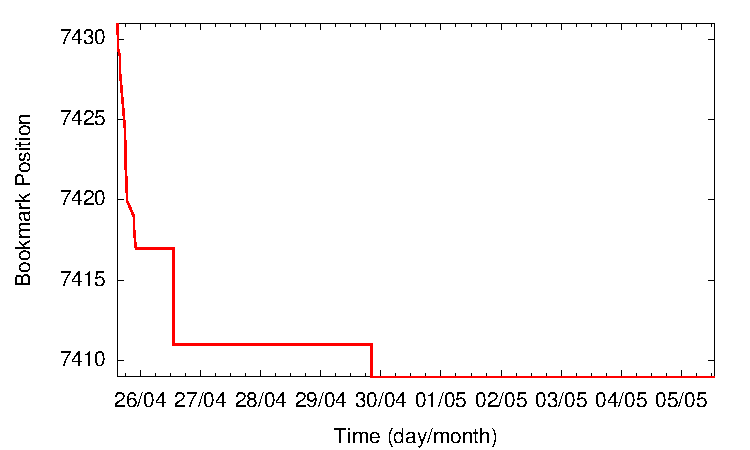
\includegraphics[width=0.5\columnwidth]{./graphs/mufc-mila_Goal_3-2_time}
    }
    \subfloat[][Position over requests for bookmarks] {
        \label{fig:man-mil-requests}
        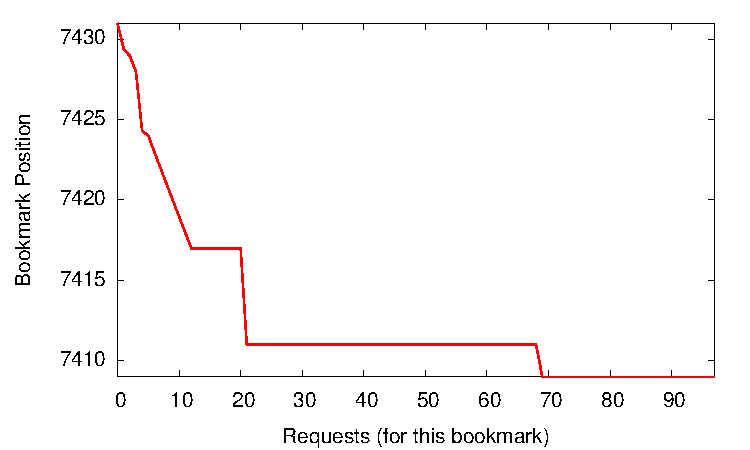
\includegraphics[width=0.5\columnwidth]{./graphs/mufc-mila_Goal_3-2_request}
    }

    \caption{Manchester United vs Milan single bookmark position}
    \label{fig:man-mil}
\end{figure*}

To test this algorithm, several of the bookmarks in the second video trial (not the initial World Cup experiment) were deliberately misplaced by different amounts before they appeared on the live site. Over time the bookmarks were moved autonomically by our algorithm. For example, \autoref{fig:man-mil-time} \& \autoref{fig:man-mil-requests} show the position of a single bookmark as it was moved by the system with respect to time and received requests. In both cases the system responds and the bookmark quickly moves to a new position, and then gradually converges until it becomes stable. In most cases the majority of movements were only in one direction, but for a couple of bookmarks the positions oscillated between two values. The most prominent example of this was a foul in a football match which led to a penalty. Some users wished to see the foul but others only wished to see the penalty a minute later. In these small number of cases it is subjective to decide if a bookmark is correctly placed, and in fact using this algorithm the bookmarks may never converge to a single point. In such cases, it may be best to bias the bookmark towards the earlier position, so both the early and later events can easily be seen.

\begin{figure*}[t]
    \centering

    \subfloat[][CDF of percentage reduction in viewing duration] {
        \label{fig:duration_saved_cdf}
        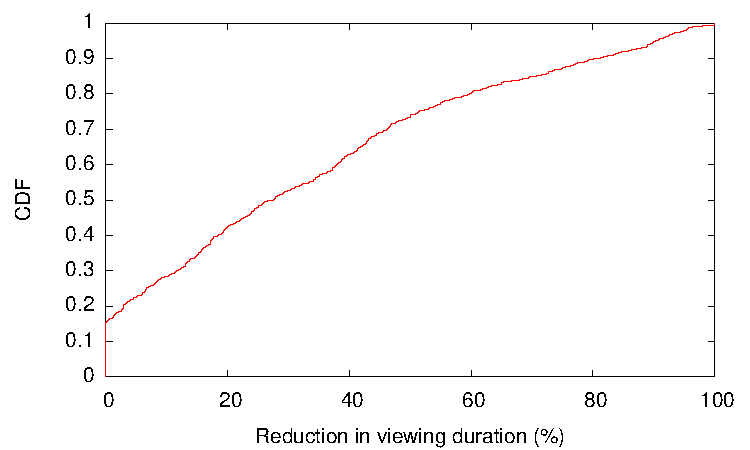
\includegraphics[width=0.5\columnwidth]{./graphs/moved_savedovertime_cdf}
    }
    \subfloat[][Percentage reduction in viewing duration versus received requests] {
        \label{fig:duration_saved_requests}
        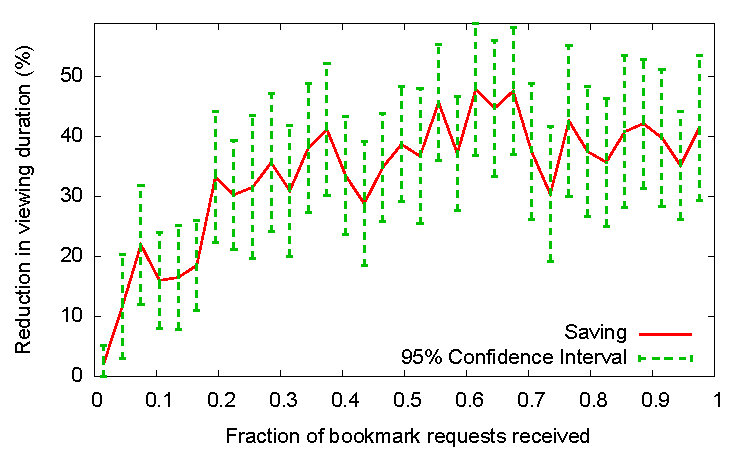
\includegraphics[width=0.5\columnwidth]{./graphs/moved_binned_savedovertime}
    }

    \caption{Reduction in viewing duration due to the algorithm}

\end{figure*}

%\todo{ Make reduction calc clearer }

Instead of subjectively deciding if a bookmark has moved to its correct location, we examined how much traffic might have been saved by moving the bookmark to a new location. If, for example, a bookmark was moved forward 10 seconds closer to the desired location, and a user views for 90 seconds, then by moving the bookmark we have potentially stopped video being transferred, which might have normally been skipped over. A reduction of $10/(90+10)=10\%$ is therefore made. Of course, this is only true if the user does not seek backward to watch the skipped 10 seconds, in which case we save nothing, and in fact incur an extra seek. \autoref{fig:duration_saved_cdf} displays a CDF of the potential reduction in viewing duration per bookmark request from the use of the algorithm. We can see that 16\% of the requests made no saving: these are accounted for by early requests before the bookmarks were moved, and requests where the user incurs an additional seek.

%seeks between the original and current bookmark location. %The remaining 84\% of request reduced the play

\autoref{fig:duration_saved_requests} illustrates how rapidly these reductions are made (and whether or not they are sustained) through a plot of the fractional potential saving versus the number of requests received across all the moved bookmarks. For the first 20\% of requests the reductions are low yet they improve, and then stabilise at a reduction of between 30-40\% per request. The 95\% confidence intervals are quite wide in most cases (averaging around $\pm$10 seconds) although this variance is mostly due to differences in playback length and not the 16\% of requests with no saving.

With minimal processing this simple algorithm has been able to reposition the bookmarks to more appropriate locations based on observed user behaviour, resulting in consistent traffic reductions. The algorithm can still be improved by fine tuning the $\alpha$ values. Larger values would move the bookmark more quickly at the cost of increasing the probability of incorrect decisions. This investigation has been left for future work.

%\begin{figure}[t]
%    \centering
%    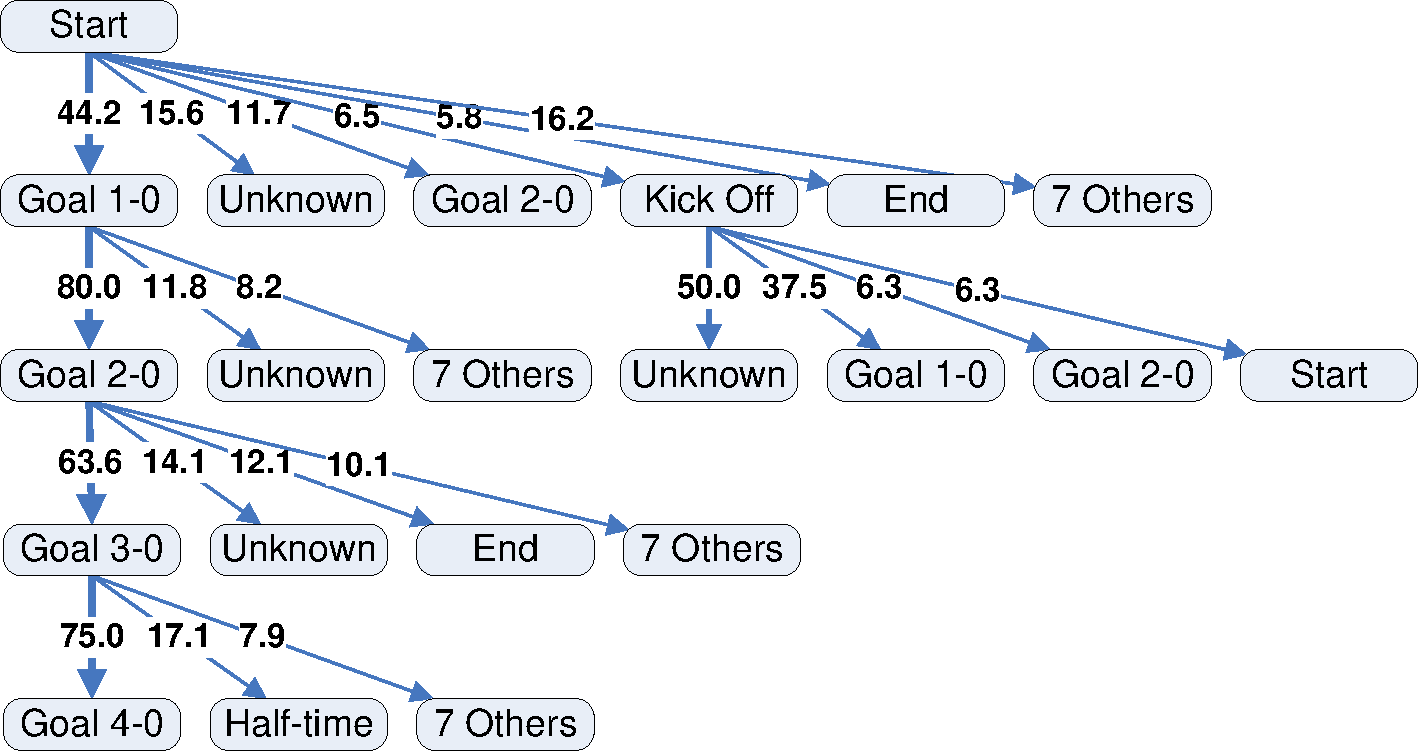
\includegraphics[width=0.5\textwidth]{./diagrams/sequence.png}
%
%    \caption{Graph of the order bookmarks are clicked. Note: This is a work in progress, and doesn't display well so I'll send links around to larger pngs.}
%%    \label{fig:mil-man}
%\end{figure}

%   Before  After   Distance            Best
%mufc-mila_Goal 1-2 3185    3168    17  Late            *interesting, because bookmark was well placed (but got moved)
%mufc-mila_Goal 3-2 7431    7409    22  Late        7417.808
%liv-che_Goal 1-0   2286.185    2187    99.185  Late
%ita-fra_Penalty 1-0    3915.718    3904    11.718  Late
%mil-man_Goal 3-0   8433.083    8415    18.083  Late
%mil-man_Goal 2-0   4505    4473    32  Late
%mil-man_Goal 1-0   3260    3277    -17 Early       3299.81

%notes
%Rates of seeks over time
%Find the end of bookmark
%change the sequence graphs (to show direction, correct weights), and possible add another "didn't jump" state
%what time do they jump out?

% How many times was a segment re-watched, and how soon between watching? Indicates how useful local buffering old content would help

%\autoref{fig:man-mil} show the position of a single bookmark in the Manchester United vs Milan over time. This bookmark was purposely placed too late by 15 seconds, causing frustrated users to rewind. \autoref{fig:mil-man} shows the placement of a Milan vs Manchester United bookmark which was placed 30 seconds too early.


\section{Predictive Pre-fetching}

In the classic start-to-finish model it is commonplace to simply pre-fetch ahead of the playback point. This reduces the chance of playback stalling due to momentary network problems. However, due to the increased interactivity of users and their departure from the start-to-finish model, it is no longer wise to only pre-fetch ahead of the playback point. As noted in \autoref{sect:sequence} it is possible to predict which bookmark a user will view next, allowing the client to intelligently pre-fetch content, benefitting both clients and servers.

For the clients, pre-fetching removes seek latency when seeking to a pre-fetched segment, both in terms of incurred network seek latency and also the time taken to buffer enough video for playback.  Pre-fetching also helps to avoid buffer underruns under poor network conditions. Similarly, on the server side, pre-fetching can help reduce the peak server load by increasing the load at quieter times with pre-fetching requests, thus making the overall load more uniform.

%Figure~\ref{fig:server_load_a} gives an example of server load at different times. The shaded areas show the server going over some limit, perhaps the server's bandwidth capacity. If pre-fetching is used this load could happen earlier whist staying below the server's limit as shown in Figure~\ref{fig:server_load_b}.

However, pre-fetching does come with a cost; resources are wasted if a segment is downloaded and never used. Deciding which segments to pre-fetch is therefore an important task. This section gives some background on the concept of pre-fetching, followed by the design and evaluation of a pre-fetching technique for our highly interactive workloads.

\subsection{Background}
    %Nic has read

    % TODO, maybe try and incorporate the following
    %"Exploring prefetching to improve the scalability of these protocols for interactive workloads is left for future work."~\cite{costa2004aci}

    % Many forms of pre-fetching
        % Pre-fetching (or Pre-loading) videos before you even request them
        % Buffering ahead of the current playback point
        % Pre-fetching segments within the video
    % Pre-fetched data may be pulled to a local STB, or a local cache server~\cite{sen99ppc,eager1999orc}
    % Pre-fetched data may be fetched from broadcast streams, server, or other nodes

    Pre-fetching or pre-loading, is the act of requesting content in advance of demand. This allows clients to have the requested media stored locally before needing it. When a client eventually does request the media, it can be served from the local cache, as opposed to requesting it from a server. Pre-fetching can therefore improve the experience for clients, as there is reduced start-up delay, at the cost of pre-fetching content which may never be viewed.

    %Servers can also benefit from pre-fetching, for example, if the content is pre-fetched when the server has spare capacity, it will hopefully reduce load at peak times.

    There are a three main forms of pre-fetching. The first is pre-fetching the media before playback. The second is when playing media, to buffer slightly ahead of the playback point. The last is to pre-fetch segments of media while the media is being played. These three forms will now be discussed in more detail.

    When the media is fetched before playback has began it is typically called pre-loading. This involves either fetching the full media, or just the beginning segments of the media~\cite{paris2001cap}. Pre-loading the beginning segments is typically used to reduce the start-up latency when the media is periodically broadcast~\cite{paris1999zdb}. The decision of what to pre-load is normally based on what content is popular, and how much spare capacity the server has. There have been numerous papers detailing the optimal parameters~\cite{barnoy2008odm}, such as how much to pre-fetch~\cite{paris2001stp}, how many objects to pre-fetch~\cite{paris2002bpv}, how much bandwidth to use, what delivery mechanism to use~\cite{chung2003evb}, \emph{etc}. From the work, it seems clear that the exact parameters are dependant on the characteristics of the media, as well as how the media is delivered. But overall, pre-fetching at least the first few minutes of media certainly provides benefits.

    A very common pre-fetching technique is to buffer ahead of the playback point. This requires a small buffer, large enough to contain at least a few seconds of media. Before playback begins, this buffer is filled and then playback may start from the buffer. The buffer smooths out playback, allowing it to be jitter free, as well as hiding temporary network problems, such as lost packets. This kind of pre-fetching is also useful when streaming variable bitrate (VBR) content~\cite{reisslein1997jsq}. Typically, VBR content is bursty, causing periods of time where the server is either under-utilised or oppositely, unable to satisfy the demands of its clients. To solve this, each client requests the VBR content at a constant bitrate (equalling the mean VBR rate), allowing the client's local buffer to smooth out the burstiness~\cite{bakiras1999sap}.

    The final technique is to pre-fetch segments which are likely to be viewed within the content. This is one of the main areas of interest in this section. The pre-fetched segments can be areas within the media which are particularly popular, and are likely to be watched. Popular segments may occur when users selectively seek within the media and do not follow the typical start-to-finish model of playback. As far as this author is aware, there has been no work which will pre-fetch segments of media in this manner.

    The closest example of such pre-fetching, is ``link pre-fetching'' used by some web browsers and proxies~\cite{chinen1997ipp}. This feature will pre-fetch hyperlinks on the web page that the user is currently viewing. In this way, if the user clicks on a hyperlink which has been pre-fetched, the page will load instantly. However, this technique has been discouraged~\cite{davison2001apg}, as most of these systems blindly fetch all hyperlinks on the page. This generates additional bandwidth, and may overload the servers~\cite{duchamp1999ph}.

    When content is pre-fetched, it is not always stored in the same place. Earlier work assumed that pre-fetched content would be stored on content servers near to the clients~\cite{sen99ppc,eager1999orc}. More recent work has assumed that clients are using a set-top box (STB) or PC to view the media, both of which may contain a large hard disk or similar storage device. This allows the content to be available even when the client has no connectivity.

    Pre-fetching does not always have to involve a server. In the most na\"{i}ve systems, pre-fetched data is requested directly from the server via unicast distribution. More advanced systems have dedicated pre-fetch channels which periodically broadcast the segments of media which the server deems useful to pre-fetch~\cite{chung2003evb}. More recently, systems have been designed to pre-fetch media from neighbouring clients~\cite{shen2006dps}. One study by Huang~\emph{et~al.} found that if peers used their spare upload to assist others in pre-fetching, the server's bandwidth could be significantly reduced~\cite{huang2007civ}.

\subsection{Pre-fetching Strategies}

The workloads observed in this thesis exhibited sparsely distributed areas of high interest. This areas have been dubbed ``hotspots''. A sensible pre-fetching strategies would take advantage of these hotspots, and pre-fetch their segments accordingly.

Therefore, a set of pre-fetching strategies were devised. For simplicity, and because interest typical formed around bookmarks, each strategy will only pre-fetch segments immediately following a bookmark (\emph{i.e.}, bookmarked hotspots). In all experiments the amount of each hotspot pre-fetched was determined by varying the percentile of that particular hotspot's length model, as described in \autoref{sect:hotspot_length}.

Each pre-fetch strategies was tested within a simulator driven by the \emph{eurovision} trace. Clients were provisioned with a dedicated link to the server, capable of transferring twice the bitrate required to play the content. Once a client has fetched enough data to fill a 5 second playback buffer, half of their bandwidth is allocated to the pre-fetcher whilst the other half continues to fill the playback buffer.

The details for each pre-fetch strategy are listed below:

%Simulations were run using real \emph{eurovision} traces obtained from our system to test these different strategies. \emph{Eurovision} was chosen due to its popularity and  representative nature. As soon as the client starts playback of a video a separate thread begins to pre-fetch segments (at playback rate) which the scheme anticipates the client will need. Connections between the clients and server were highly provisioned and never congested. In all experiments the amount pre-fetched for each bookmark was determined by varying the percentile of that particular bookmark's length model, as described in Section~\ref{sect:hotspot_length}.

%We used different pre-fetching strategies, each using different information to decide which segment to fetch next. For simplicity, and because interest always formed around bookmarks, each strategy will only pre-fetch segments immediately following a bookmark (bookmark hotspots). %Hotspots always focused around bookmarks therefore these were a good choice to prefetch. However the length of these hotspots were not always know, so as you will see later, arbitrary values were used for the length of the pre-fetched segment.
%The different pre-fetching strategies tested are explained as follows:

%    \textbf{Before Start} pre-fetches all the bookmark hotspots before the user begins any playback. This demonstrates how well pre-fetching everything in advance will perform.

%    \textbf{Best} uses knowledge of future events to pre-fetch the bookmark hotspot that the user is actually going to view next. This is impossible to implement in practice, so this technique is for reference only. %Similar to Belady's minimum.

\begin{description}
  \item[Ahead] simply continues to pre-fetch ahead of the playback point assuming the client has a unlimited buffer. This is similar to what most existing streaming applications do.

  \item[Ahead (to hotspot end)] again simply continues to pre-fetch ahead of the playback point but only until the end of hotspot associated with the bookmark being viewed.

  \item[Ahead (and Predictive)] works in a similar way to \emph{Ahead (to hotspot end)}, however, once it reaches the end of the hotspot it begins to use the \emph{Predictive} pre-fetch scheme.

  \item[Predictive] uses knowledge observed from other users as to which bookmark is likely to be requested next, and thus starts to pre-fetch the bookmark hotspots in descending order of probability of being visited. This uses the sequence tree concept introduced in \autoref{sect:sequence}, therefore the more users interacting with the system, the more accurate the predictions becomes.

  \item[Sequence] will pre-fetch bookmark hotspots in the order in which they appear within the video regardless of the current playback point. For example, in a football match the bookmarked goals would be pre-fetched in a sequential order.

  \item[Sequence After] again pre-fetches bookmark hotspots in the order in which they appear within the video; the difference being only hotspots that are after the current playback point are fetched. For example, if a user has yet to fetch the first bookmark's hotspot but is already viewing the second, then the first will not be pre-fetched.

%  \item[Random] will pre-fetch the bookmark hotspots in a random order.
%  \item[Popularity] pre-fetches the bookmark hotspots in order of their overall popularity.

\end{description}


%Simulations were run using real \emph{eurovision} traces obtained from our system to test these different strategies. \emph{Eurovision} was chosen due to its popularity and  representative nature. As soon as the client starts playback of a video a separate thread begins to pre-fetch segments (at playback rate) which the scheme anticipates the client will need. Connections between the clients and server were highly provisioned and never congested.

\begin{figure*}[t]
    \centering

    \subfloat[][Fraction of requests with zero seek latency] {
        \label{fig:eurovision_instaseek}
        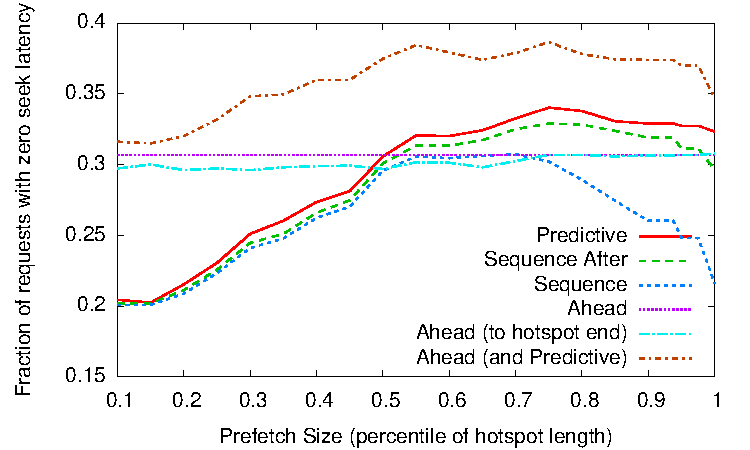
\includegraphics[width=0.5\columnwidth]{./graphs/1206722178-eurovision_tab-instaseek}
    }
    \subfloat[][Usage ratio] {
        \label{fig:eurovision_usage}
        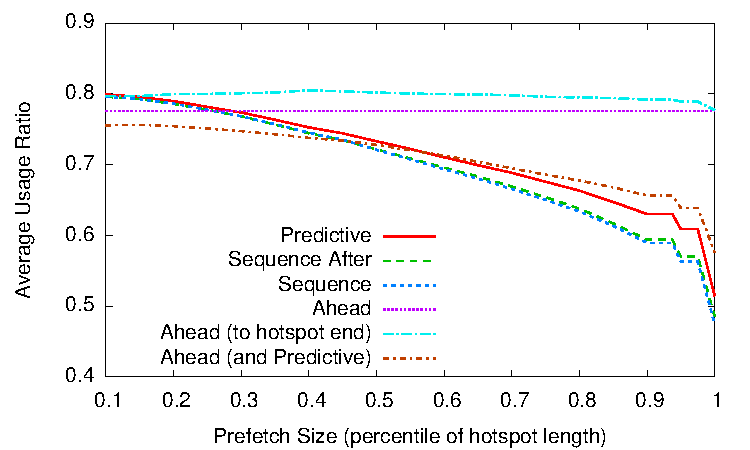
\includegraphics[width=0.5\columnwidth]{./graphs/1206722178-eurovision_tab-usage}
    }

    \caption{Various metrics for different pre-fetch schemes versus bookmark length}

\end{figure*}

Two metrics were measured to determine how well the different schemes behaved. The first metric displayed in \autoref{fig:eurovision_instaseek} is the fraction of requests with zero seek latency. A seek latency of zero occurs when the user has already pre-fetched a playback buffer's worth of video from a requested seek point. The second metric measured the ratio of fetched data which was never watched, and therefore needlessly fetched. This usage ratio is shown in \autoref{fig:eurovision_usage}.

Using the simple \emph{Ahead} scheme 31\% of seeks have zero latency, this is made up of seeks to segments that have already been viewed, and small forward seeks into the ahead buffer. Adapting this scheme to only pre-fetch to the end of the bookmarks (\emph{i.e.} the \emph{Ahead (to hotspot end)} scheme) has a minor negative effect on the seek latency, whilst increasing the average usage ratio.

The \emph{Sequence} and \emph{Sequence After} schemes are very similar, but the simple modification to the \emph{Sequence After} scheme allowed it to achieve a lower seek latency whilst not degrading its average usage ratio. This was because users had a tendency to not seek to a bookmark before the current playback point, and always go forward within the video, leaving the \emph{Sequence} scheme stuck pre-fetching hotspots before the current playback point.

Both the \emph{Predictive} and the \emph{Sequence After} schemes perform in a similar manner, with the \emph{Predictive} schemes always outperforming the other. Due to this fact, the \emph{Sequence After} scheme could be used in place of the \emph{Predictive} scheme whilst knowledge is collected to improve the \emph{Predictive} scheme's accuracy.

The best outcome was the combination of \emph{Ahead} and \emph{Predictive} schemes named \emph{Ahead (and Predictive)}. This exploited the fact that users rarely viewed beyond the end of a hotspot, and thus pre-fetching another hotspot was of benefit.



%This has left unanswered however if pre-fetching segments based on the beginning of the bookmark is the best solution, whereas pre-fetching smaller grained segments might be better.
%So far these results look promising, however there is room for improvement.

%As expected, the \emph{Before Start} and \emph{Best} schemes outperformed all others. The \emph{Predictive} and \emph{Sequence After} schemes both performed equally catching at most 23\% of seeks, and the \emph{Popularity}, \emph{Sequence} and \emph{Random} schemes also performed equally albeit roughly 5\% lower than the \emph{Predictive} and \emph{Sequence After} schemes.
%It is interesting to note that using the popularity of the bookmark is not as effective as using the somewhat na\"{\i}ve \emph{Sequence} scheme. This is because while the \emph{Popularity} scheme is pre-fetching the most popular bookmarks (which could be towards the end of the video), the \emph{Sequence} scheme is fetching closer bookmarks which will be used sooner.
%As the pre-fetch size becomes larger most schemes are able to offer more zero latency seeks due to aiding seeks that occur shortly after the bookmark (\emph{e.g.}, seeking 15 seconds forward). However the improvements begin to diminish around 60\% as excess data is pre-fetched and thus time would be better spent fetching a different bookmark.

%Each scheme may pre-fetch different amounts of data. For example, the \emph{Best} scheme will keep trying to pre-fetch the bookmark hotspot that the user will view next, but if there is no following bookmark the scheme stops pre-fetching. Figure~\ref{fig:eurovision_usage} displays the amount pre-fetched data that was actually used for playback. The \emph{Best} scheme performs at least twice as well as any other listed, with the \emph{Before Start} performing worse since it has pre-fetched far more data than actually gets used. From the remaining schemes, \emph{Predictive} is consistently the best, achieving between 31\% and 39\% usage.
%
%Finally, we observe the overall byte hit/miss ratio in Figure~\ref{fig:eurovision_ratio}. This is how many bytes were successfully served by pre-fetched data versus the total number of bytes requested. Again, the different schemes performed similarly, with \emph{Predictive}, \emph{Sequence After}, and \emph{Popularity} performing equally. However, none of the schemes, including \emph{Before Start} achieved a satisfactory hit-ratio. At best, the realistic schemes achieved less than 20\%. This may be because the bookmark hotspots do not sufficiently cover the area requested by the users. Future work could therefore incorporate strategies that pre-fetch more than just hotspots following a bookmark.
%
%From these results it is clear the \emph{Predictive} and \emph{Sequence After} schemes perform best, with the \emph{Predictive} scheme slightly outperforming \emph{Sequence After} by having a higher pre-fetched utilisation. One aspect that has not been investigated is how quickly reliable knowledge needed for the \emph{Predictive} scheme can be obtained through other users' interactions. As such, a hybrid approach could be taken, beginning by using the simple yet effective \emph{Sequence After} scheme, switching to the \emph{Predictive} scheme once sufficient statistics have been acquired.
%
%The \emph{Best} scheme outperformed all others which suggests room for improvement in the other pre-fetching algorithms. The results presented are, however, perhaps the worst case since each client is working independently. If the clients collaborated, a shared pre-fetching network cache could result, thus increasing the hit/miss ratios while decreasing the load on the CDN.

\subsection{Pre-fetching Knowledge}

\begin{figure}[t]
    \centering

    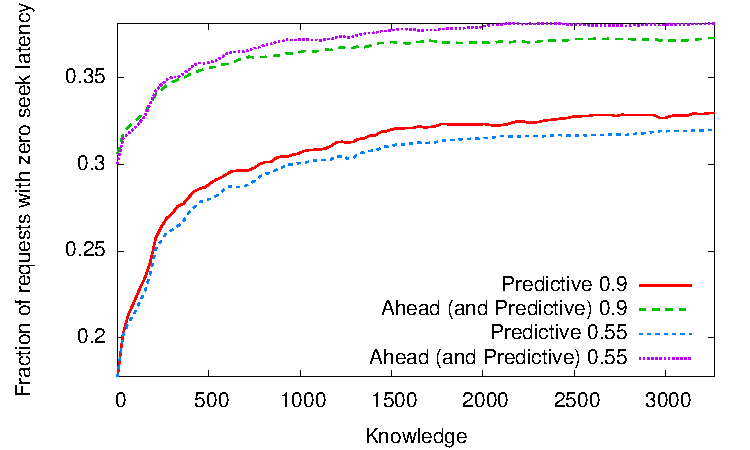
\includegraphics[width=0.5\columnwidth]{./graphs/1206982048-eurovision_tab_average-seek-knowledge}

    \caption{How zero seek latencies is effected by amount of pre-fetch knowledge}
    \label{fig:eurovision_knowledge}

\end{figure}

In the previous experiments the \emph{Predictive} scheme was primed with knowledge from all users, but in reality this knowledge would be built up over time. To test how quickly this knowledge could be obtained, we ran another set of experiments where the \emph{Predictive} and \emph{Ahead (and Predictive)} schemes were primed with different amounts of knowledge. The results of this are shown in \autoref{fig:eurovision_knowledge}. We set the percentile hotspot length to 0.55 and 0.9, which were chosen since 0.55 is where the seek latency began to stabilise, and 0.9 is where the usage ratio began to drop rapidly. The knowledge is ranked from 0 to 3000 which represents the number of seek requests the knowledge was based on. It can be seen that very quickly (within 250 seek requests) the knowledge has become useful, and eventually plateaus at 1500 seek requests. Any seek requests after this point just increase the confidence in the knowledge and does not improve it.

\begin{table}[tb]
\centering {
    \begin{tabular}{|cccc|}
      \hline
\setrowcolor{TableRowHead}
      Media & From (seconds) & To (seconds) & Frequency \\
      \hline
\setrowcolor{TableRowA}
      arg-scg  & 0    & 1024 & 34 \\
\setrowcolor{TableRowB}
      arg-scg  & 0    & 271  & 10 \\
\setrowcolor{TableRowA}
      arg-scg  & 0    & 0    & 5 \\
\setrowcolor{TableRowB}
      arg-scg  & 271  & 1024 & 8 \\
\setrowcolor{TableRowA}
      arg-scg  & 279  & 1024 & 2 \\
      \hline
    \end{tabular}
} \caption{Example links table, showing the frequency of seeks from one time to another}
\label{tab:links}
\end{table}

In a real system, predictive knowledge must be collected in real time, and then disseminated in an efficient, scalable, and quick way otherwise any benefits gained may be lost in overheads. One solution to gathering this knowledge is described below.

% Nic prove read on 9th Sept (all but last 2 paragraphs)

To gather this knowledge, the clients and servers must store a small amount of state. Clients must record what is currently being requested. These details are typically recorded by the client anyway, for example, the name of the media, as well as the location playback started within the media. To make the solution scale, and generate less overhead for the server, it has purposely been designed so that the server need not store per-client state. The servers must only store a table of links relevant to the media stored on that server.

An example of the server's links table is shown in \autoref{tab:links}. This table maps the frequency of seeks between two locations within the media. For example, \autoref{tab:links} shows that 34 seeks occurred between time 0, and time 1024 within the \emph{arg-scg} media. This table may be used by the server or clients to predict what they will visit next, for example, if a user has just started playback of \emph{arg-scg}, they have a $34/(34+10+5)$ or 69\% probability of seeking to time 1024 within the media.

To construct this table the client must send some additional information to the servers. Typically when a client seeks, a new request is issued and the old request is stopped. This new request may be issued to a different server if the media is partitioned across multiple servers, or just for load balancing purposes. So when a client issues a new request, it must send details of the new seek location to the previous server. These details can be sent when the client stops the previous request.

By sending details of the new request, the previous server is able to infer a link between the two requests, even if the next request is supplied by a different server. The server does not need to store any additional per-client state, at the cost of trusting that the client will always send correct information. The inferred links can be stored in a table along with the frequency of their occurrences. This is the beginning of constructing a prediction tree. Once sufficient links have been inferred, a tree can be constructed.

Once this links table begins to be constructed, it can be used by both the servers and clients. When a user makes a request, the server can send a subset of the table to the client as out-of-band data. For example, if the client requests second 0, then the server would send the subset of rows whose \emph{from} time is 0. This would give the client the knowledge to predict which locations are most likely to be visited following the current location. As the client continues playback, the server can send additional subsets of the table. For example, if the client continued playback for a further 60 seconds, then subsets of the table from time 60 will be sent, again as out-of-band data.

When multiple servers are used, the links tables can easily be shared or partitioned among the servers. If two servers create the tables independently, they can be easily aggregated to produced more accurate data. The frequency of sharing the links table is left for future work.

\begin{figure}[t]
    \centering

    % Plotted with PlotLinkFrequencyCDF

    \subfloat[][Link Frequency (Absolute)] {
        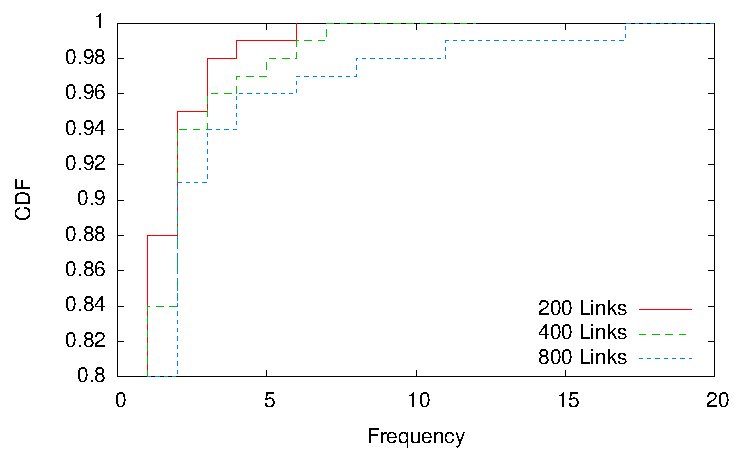
\includegraphics[width=0.5\columnwidth]{./graphs/arg-scg-cdfs}
        \label{fig:link-freq-a}
    }
    \subfloat[][Link Frequency (Normalised by from time)] {
        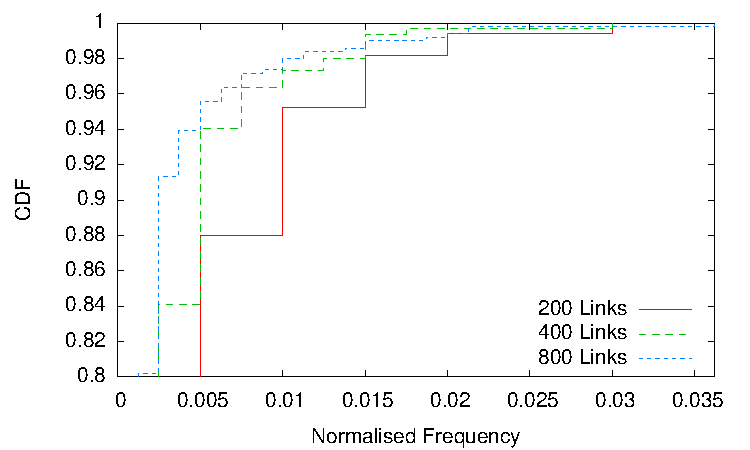
\includegraphics[width=0.5\columnwidth]{./graphs/arg-scg-cdfs-norm}
        \label{fig:link-freq-b}
    }

    \caption{CDFs of Argentina vs. Serbia and Montenegro link frequencies with varying numbers of links in the table}
    \label{fig:link-freq}
\end{figure}

The size of these tables may quickly be filled with requests with only a small frequency. \autoref{fig:link-freq-a} displays a CDF of link frequencies for one table with varying number of links in it. It can be seen that when there are 800 links, roughly 80\% of these have a frequency of one. These small frequencies may not be useful. Therefore, there are a few ways to reduce the size of the table. The first technique will reduce the resolution of the table by grouping similar times together. For example, in \autoref{tab:links}, the values 271 and 279 could be rounded down to a single value of 270. Then all matching values can be easily aggregated. This technique would most likely be used to at least round down to the nearest keyframe. As playback of media can only start from a keyframe, then it makes sense it always round the \emph{from} and \emph{to} times to the nearest preceding keyframe.

The second method aims to remove ``noise'' from the data. Each frequency can be transformed by some operations, such as a division or a right bit shift. Any frequencies which become zero or less would be removed from the table. Any values large enough to be significant will be kept, and the long tail of small results will be lost. A count of how often the table is reduced in this way must be kept to enable the table to be aggregated easily with other servers.

A final suggested technique would use the concept of aging, whereby entries in the table that have not be observed recently are removed from the table. This technique may provide the most relevant entries at the cost of additional overhead for each entry.

An evaluation of these techniques has not been conducted in a real system, and is therefore left for future work. However, the system has been designed to be lightweight and take advantage of how the delivery systems normally operate. The client, for example, only needs to send a small amount of additional information piggy-backed on existing communications. Additionally the servers do not have to handle any ``heavy'' per-client state, and instead only store the links table, which even if large would only consume 10-50~kilobytes\footnote{Based on 12~bytes per row, and between 800--4000 rows.} per media object.

%\todo{Put the results of these method here!!!!}

\section{Hybrid Delivery}

This section discusses how existing peer-to-peer (P2P) delivery techniques are unable to provide a sufficient level of interactivity to adequately support the workload analysed in this thesis. To improve the performance of P2P delivery, this section discusses a hybrid approach which can use the best features of two main classes of streaming P2P. These two classes are `pull' and `push', which have previously been described in \autoref{sect:peer-to-peer}.

To recap, push based systems configure the peers in a tree topology, and disseminate the content efficiently throughout the tree. This however does not give the peer freedom to seek within the stream, as everyone in the tree is at the same playback point. To seek, the peer would therefore need to join another tree, causing long seek delays.

The pull based system do not typically try to configure the peers into any structured way, instead creating random meshes of connections between the peers. Each peer must advertise the segments of the media they currently have stored locally. Peers may then request these segments arbitrarily, allowing them to play back the media in a sequential manner, or if they wish, seek to any segment and resume from there. This however requires a high amount of overhead as segment advertisements must be continually exchanged and each segment is only received after an solicited request.

The remainder of this section describes a hybrid approach which constructs the peers into multiple push-based trees using a periodic broadcast technique. The peers also form a light weight pull-based mesh, so they can use a P2P patching technique to allow for quick seeking. The following section describes these typically multicast/server orientated broadcasting and patching techniques, and how they relate to peer-to-peer. Following this, design, analysis and evaluation of the hybrid scheme is discussed.

\subsection{Periodic Broadcast and Patching}
    %Nic has read

    It is cheaper in terms of resources to serve ten users via a single multicast stream, then to serve the same ten users via unicast. Creating a single multicast channel decreases network load, as only $1/10$ of the bandwidth is needed, and also reduces requirements placed on the the server, such as the memory and disk IO bandwidth. However, it is not always possible to ensure that the users all wish to start watching at the same time; batching was therefore created to solve this~\cite{dan1994spf,aggarwal1994apb,viswanathan1996mav,hua1996sba}.

    Batching in its simplest form groups users with the same playback point together and delays them receiving the media until a suitable multicast stream can be found/created to accommodate the full group. This works well if the media is periodically broadcast~\cite{chiueh1995pba} on multiple multicast channels at fixed intervals apart. This technique is also called staggered broadcasting. When a client joins or seeks to a specific point~\cite{grant1994mpv}, they wait until one of the channel's playback points matches their required playback point. However, this causes a long delay, for example, if a 60~minute video is broadcasted over 10 evenly distributed channels, it can take at most 6 minutes to view any requested location, but on average only 3 minutes. To allay this issue, enhancements such as harmonic broadcasting~\cite{juhn97hbv} or patching can be employed.

    Patching (or sometimes called Stream Tapping~\cite{carter1997sta}) extends batching by adding a mechanism to remove the start-up delay whilst still utilising multiple dedicated channels~\cite{hua1998pam}. When a client requests a playback location which can not instantly be served by an existing channel, a separate patching channel is created. This can occur when the client first views the content, or if they seek to an arbitrary point. The client then requests both the patching channel and a dedicated channel whose playback point is later than the requested playback location. The patching channel contains the data required to catch up with the dedicated channel and is typically unicast from a content server or sometimes from neighbouring clients~\cite{kulkarni2008ast}. This then allows the client to begin playback instantly from the patching channel and buffer from the dedicated channel. Once the patching channel catches up with the client's buffer, the patching channel is stopped.

    The idea was extended to reduce the number of required dedicated channels. For example, consider there are two dedicate channels one being 10~minutes behind than the other. If a client is currently viewing the channel which is behind, they may start to patch from the ahead channel. After 10~minutes they would have caught up with the ahead channel and thus can disconnect from their behind channel. This then might allow the channel to be freed if no other users are viewing it.

    The duration for which the patching channel is used is called the \emph{patching window}~\cite{cai1999opp}. The size of the window can impact performance, for example, the \emph{greedy patching} scheme tries to minimise the number of multicast channels by allowing the patching window to be as long as the content's duration. It has been shown that being too greedy can result in less data sharing~\cite{hua1998pam}. The opposite of greedy patching is \emph{grace patching}, which schedules a new multicast channel when the client's buffer is smaller than the patching window.

%~\cite{gao1999siv}  eager2001mbr griwodz2000tlp
    A middle ground is controlled multicast, which adds access controls limiting how many patching channels can be created. For example, the controlled \emph{CIWP} algorithm~\cite{gao1999siv} uses a mathematically optimal scheduling algorithm that limits the rate at which patching channels are created. Another technique, Lambda Patching~\cite{griwodz2000tlp}, allows the server to decide on the patching window sizes, based on currently observed popularity and interarrival times.

    A final scheme is \emph{transition patching} which increases the size of the patch window, but allows multiple clients to share a patch stream, thus increasing bandwidth sharing~\cite{cai1999ebs}. The efficiency of these patching schemes has been measured~\cite{bradshaw2001pba, eager2001mbr}, modelled~\cite{tan2002qos} and optimised when considering factors such as video length, client buffer size and request rate~\cite{cai1999opp, eager1999oae, sen1999ops}.

    Although patching was originally designed to provide simple video-on-demand, it also enables interactivity. More recently, Ma~\emph{et~al.} optimised patching for high levels of interactivity~\cite{ma2005bep}. However their evaluation used non-realistic interactivity patterns. Rocha~\emph{et~al.} tested patching with more realistic interactive patterns and found that patching did not scale well under high levels of interactive requests. With low levels of interactivity, patching performed sufficiently. However, with medium to high interactivity, patching performed in a similar way to serving each client with an individual unicast stream~\cite{rocha2005sms}.

    %Piggybacking, speeds up one stream by a small amount, ie 10\% to allow it to catch up with another.

% Golubchik, L., J. Lui, and R. Muntz. Adaptive piggybacking: a novel technique for data sharing in video-on-demand storage servers. ACM Multimedia Systems Journal, 4(3): 140�155, 1996.
% P�ris, J.-F. An interactive broadcasting protocol for video-on-demand, Proceedings of the 20th International Performance of Computers and Communication Conference, pages 657�664, April 2001.

\subsection{Delivery Methods}

To compared a peer-to-peer hybrid approach to the existing push and pull methods, three delivery mechanisms are defined and evaluated. This section describes the three mechanisms in detail.

\subsubsection{Push -- Periodic Broadcast over TBCP}

The first of the three approaches aims to group similar users together on a multicast substrate. Given the lack of support for network multicast, we use an application-level multicast (ALM) algorithm, specifically the Tree Building Control Protocol~\cite{mathy01otb}, which in practice is a protocol to arrange the peers in a push-based P2P tree.

\emph{Periodic broadcast} can then be used in order to provide the illusion of true video-on-demand. Staggered broadcast is its simplest form, involving a number of multicast channels for a given video, and beginning each at an interval evenly distributed throughout its length~\cite{dau95cab}. Users may then move forwards and backwards throughout the stream by switching channels. The granularity of these operations is, however, limited by the interval between the available channels. Without allocating a large number of broadcast channels, startup/interaction latency may be unacceptable in longer pieces of media. An adaptation of this method is our push approach to delivering the media, in that content nodes broadcast the same segments of content to as many nodes as possible simultaneously, where TBCP trees are generated as required to act as periodic broadcast channels.

\subsubsection{Pull -- Peer-to-Peer}
\label{sect:pull}

The second delivery method considered, representative of the pull approach to delivery, is the use of a peer-to-peer, BitTorrent-like protocol. BitTorrent implements a tit-for-tit incentives mechanisms, to discourage free-riders\footnote{Peers who chose to not contribute to the network, thus obtaining a service at no cost to themselves.}. A beneficial side-effect of involving time-sensitive data in such a network is that the incentives that drive the system become more pronounced. In other words, due to the tit-for-tat exchange mechanism,  would be encouraged to contribute, as to improve the probability of receiving the segments they require in a timely fashion. Such protocols are not without drawbacks in the context of streaming media, however.

Firstly, the most common issue is that media playback requires sequential segments of a piece of content; BitTorrent instead delivers them effectively randomly. A solution often proposed to handle the need for sequential delivery is to apply a sliding-window to the data being distributed. Peers then have upper and lower boundaries for the segments which they are interested in downloading, and prioritise their requests accordingly.

Secondly, startup latency should be minimised; BitTorrent's reliance on other peers optimistically unchoking newcomers means this is not the case. Shar~\emph{et~al.} and Vlavianos~\emph{et~al.} amongst others have noted and responded to issues such as these~\cite{shar07ppm,vlavianos06beb}. A simple solution is to ensure that established peers perform optimistic unchoking on a more regular basis; Shah and P\^{a}ris show that, when combined with a sliding window approach, significant improvements over the base protocol can be achieved~\cite{shar07ppm}. We therefore employ similar methods to gain the same benefits.

\subsubsection{Hybrid -- Periodic Broadcast with P2P Patching}

Finally, the third method examined is a hybrid of both the push and pull methodologies. By using TBCP-based periodic broadcast trees in conjunction with peer-to-peer patching, clients can share data enabling them to reach the current broadcast point rapidly. To clarify, when a client joins a periodic broadcast channel, they do not need to wait for channel to reach the desired playback point, but can instead request segments from their neighbours as quickly as possible until the broadcast channel reaches the required position. This system is similar to the one described by Guo and Ammar~\cite{guo2004slv}. They used periodic broadcast over ALM, supported by server based patching. They showed promising results, however, their workload was an artificial start-to-finish.

\subsection{Experiment}

Three key variables to be considered for a delivery system are the size of the audience, the nature of the content (workload) and the network resources available. We also vary \emph{peer-to-peer usage}, in terms of the number of connections they are allowed to make to other peers. For example, if in an unrestricted environment there were 200 peers, a value of 10\% P2P usage would reduce the number returned to just 20. By varying this value, the effect of peer-to-peer patching on the hybrid method can be observed: at 0\% usage, the method is identical to the normal periodic broadcast over ALM, whereas at 100\% usage, the peer-to-peer scheme is made use of as much as possible. The increasing effect of the peer-to-peer patching system in the hybrid approach can therefore be observed in an incremental fashion relative to both the pure ALM and pure P2P delivery methods. Naturally, this does not affect the pure ALM approach, as no variance is seen in its results for plots of this type.

%\subsection{Workloads}

To obtain results that provide a comparison of how particular delivery schemes may handle different pieces of content, varied workloads are considered. These can be classified as follows:

\begin{description}
  \item[Start-to-Finish] Used for baseline comparison, where clients do not use any interactivity features. Media is viewed in a start-to-finish fashion, although the start and end points are not necessarily the same between clients.

  \item[Interactive] This workload is derived from the analysis and modelling conducted in \autoref{chap:evaluation}. In essence, the unique aspect of these workloads is large pieces of content with relatively short areas of high interest, highlighting how well a particular approach handles large differences in popularity between segments.
\end{description}

%\subsection{Metrics}

Beyond the workloads, the metrics used are selected to reflect both network provider and user satisfaction, based on resource usage efficiency and perceived quality of service respectively. The first metric considered, therefore, is \emph{network stress} in terms of the amount of data delivered on the network, normalised to the worst case in a given simulation.

The second metric used is `timely' segments, \emph{i.e}, one which arrived before its playback deadline. An \emph{average fraction of timely segments received per client} is therefore the average value, on a per-client basis, for the total number of timely segments divided by the total number of segments required by that client.

Finally, \emph{segment utility} is considered: the number of media segments actually used in playback in comparison with the total number sent over the network. Given that a client may receive segments superfluous to their requirements (\emph{e.g.}, buffering five minutes when the client only watches one. This metric provides a measure of network efficiency relative to the data that clients actually consume.

%\subsection{Overview}

A high-level overview of the experimental setup is as follows: 1,000 routers exist in a GT-ITM generated topology graph~\cite{gtitm}. The graph is of a realistic transit-stub configuration, wherein a single node exists per transit domain, but many exist per stub. Content node(s) (those sourcing the media) are attached to the aforementioned transit node(s), whereas clients are attached to randomly selected members of the stub domain(s). The content node(s) are connected via highly provisioned links, whereas, the clients are limited to a typical asymmetric link (1Mbit down, 256kb up).

The group size used in the simulations is 500 clients, and delivery of some subset of the piece of content per client is made using the appropriate method described for each simulation. Each client possesses an individual playback buffer, which should not underflow if user-satisfaction is to be achieved.

In our custom simulation environment, the overall delivery process is modelled in a number of steps over several iterations, whereas the content itself is handled as a series of sequential `segments'. Firstly, a realistic workload is generated (according to the models from \autoref{chap:evaluation}), wherein the clients are provided with individual lists of segments they will be required to obtain within the timeframe of the simulation.

Following workload generation, clients must interact with the delivery structures to begin the acquisition of segments. In the pull peer-to-peer approach, delivery proceeds as described in \autoref{sect:pull}. The push and hybrid approaches, however, primarily use TBCP periodic broadcast trees, meaning the initial step is for clients to determine which tree(s) will contain the segment(s) they require, and where they are rooted (\emph{i.e.}, the address to join). In the simulations this is achieved through a lookup process on a single node for simplicity, although in a real-world deployment with numerous videos of many segments each, a more sophisticated arrangement may be appropriate.

Following location of the correct tree for the required segment(s), a client must then wait on the periodic broadcast to roll-around to the required playback point for consumption. In the hybrid approach, the peer-to-peer mechanism can now be used to speed this process somewhat, by attempting to rapidly patch required segments that the client would otherwise have to wait for. Note that clients also have to use the knowledge of segment-tree mappings obtained from the lookup service to anticipate when trees must be switched, as to avoid suboptimal resource usage through nodes being present in a tree unnecessarily.

\subsection{Results}

\begin{figure}[t]
    \centering

    \subfloat[][Network cost of delivering] {
        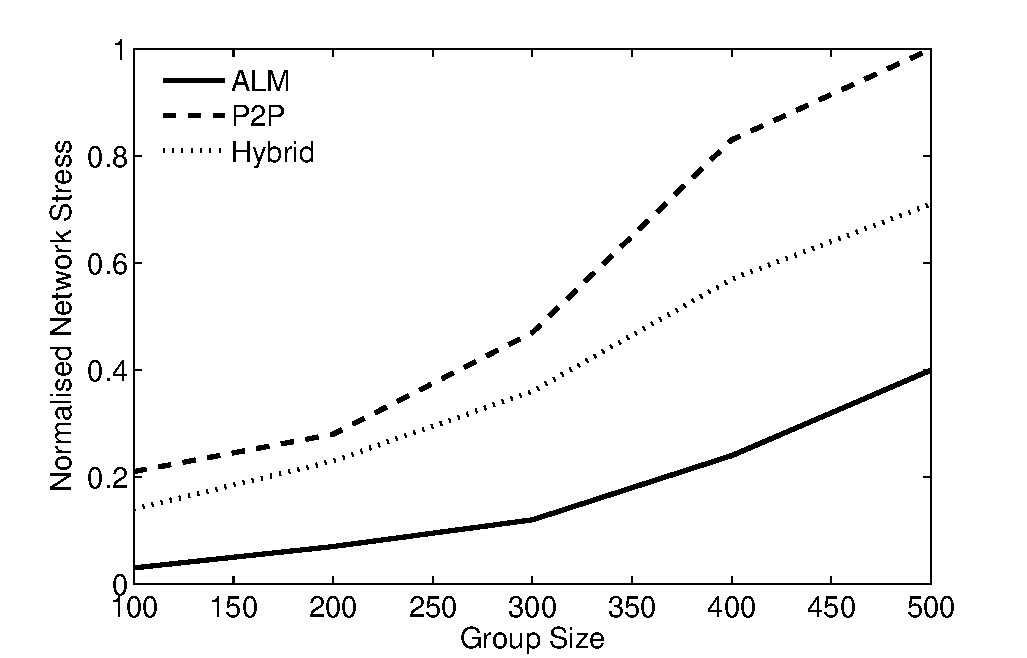
\includegraphics[width=0.5\columnwidth]{./graphs/netintsize}
        \label{fig:netintsize}
    }
    \subfloat[][User satisfaction during delivery] {
        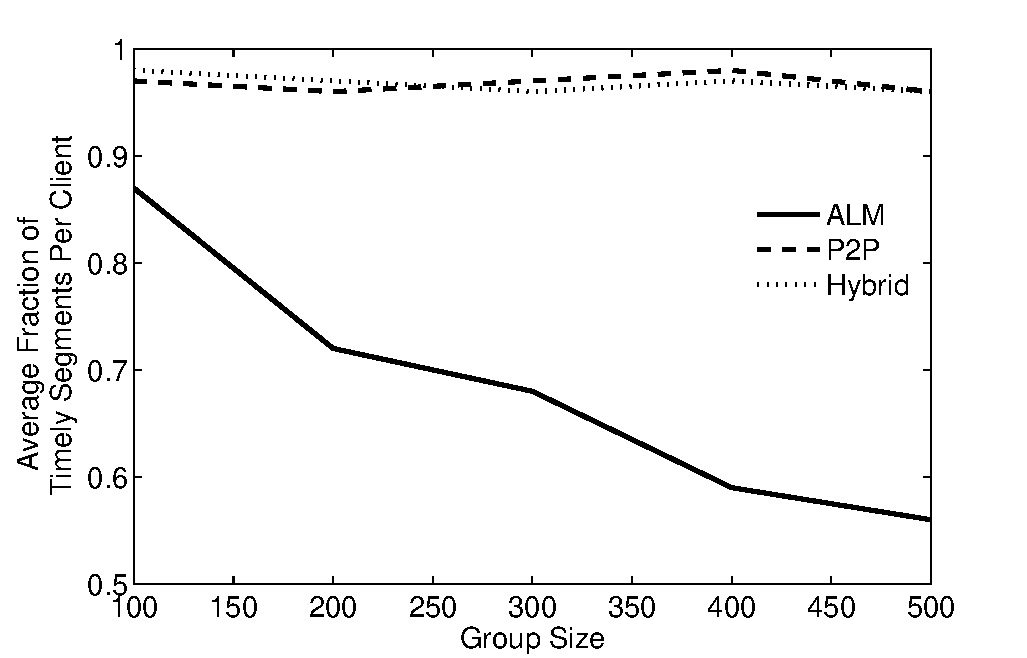
\includegraphics[width=0.5\columnwidth]{./graphs/userintsize}
        \label{fig:userintsize}
    }
    \caption{Delivering a Interactive workload with varied group size}
\end{figure}

\autoref{fig:netintsize} shows the resulting network cost across the delivery methods for an interactive workload with varying group sizes. The amount of traffic created for the ALM-based methods is shown to be lower than pull peer-to-peer; significantly so for large groups. A delivery method being low cost, however, is of little use unless it can deliver an equivalent quality of service. \autoref{fig:userintsize} shows that this is not the case for pure ALM, as an initially high level of timely segments reduces rapidly with increasing group size. Such a result may be indicative of this approach being unable to handle large, interactive groups well, possibly due to the joining overhead associated with switching between highly populated broadcast trees. Indeed, when delivering a `start-to-finish' workload (not shown), pure ALM was found to provide a level of performance similar to the other methods for the considered metrics.

\begin{figure}[t]
    \centering

    \subfloat[][Delivery of an interactive workload] {
        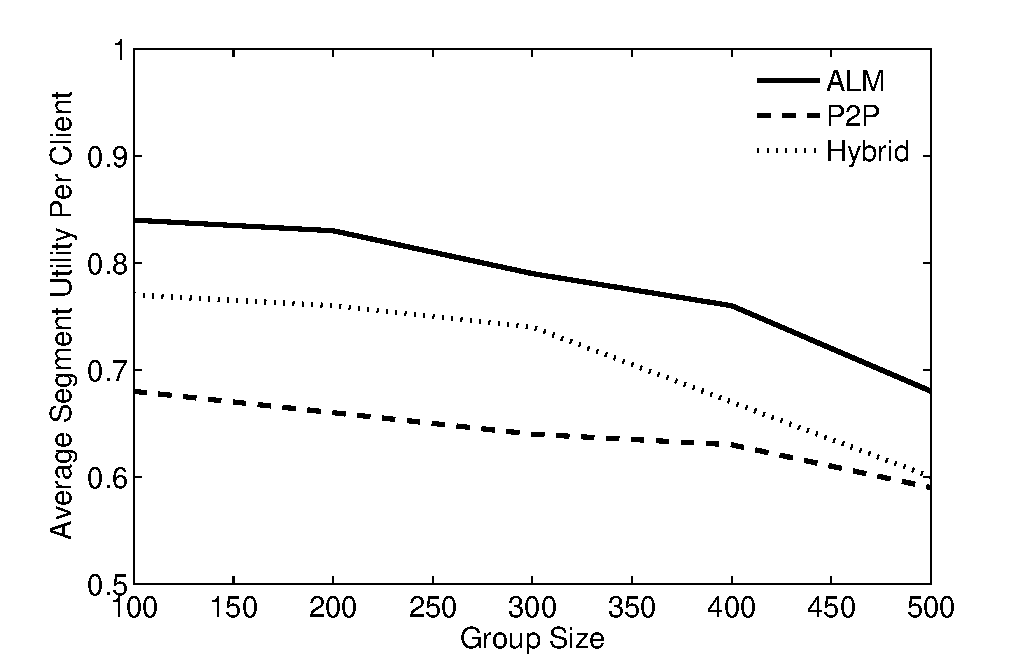
\includegraphics[width=0.5\columnwidth]{./graphs/utilintsize}
        \label{fig:utilintsize}
    }
    \subfloat[][Delivery of a start-to-finish workload] {
        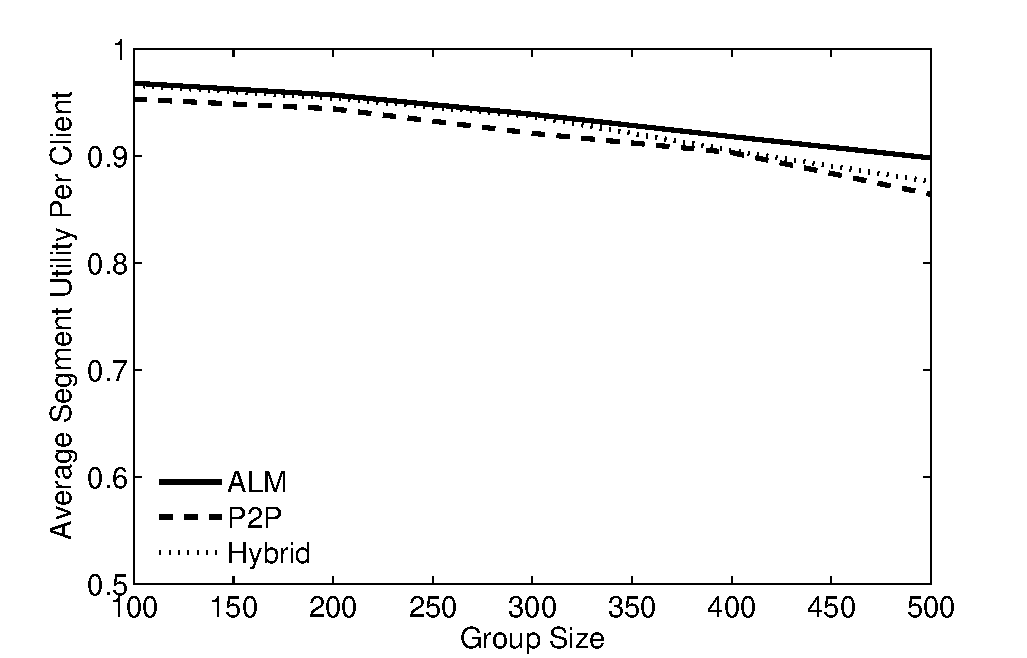
\includegraphics[width=0.5\columnwidth]{./graphs/utilstfsize}
        \label{fig:utilstfsize}
    }
    \caption{Overall segment utility during delivery with varied group size}
    \label{fig:util_size}
\end{figure}

% How can Pull/Hybrid have lower "segment utility" than push? Surely only the segments needed
% would actually be requested in pull. Perhaps they arrive late? But no, because that contradicts figure 5.7b
% Could have low utility of buffered, and this buffer was thrown away

\autoref{fig:util_size} show the average fraction of useful segments that were delivered during each simulation on a per client basis. Interestingly, \autoref{fig:utilintsize} indicates that for a high-interactivity workload, up to 40\% of segments on the network could be sent fruitlessly, with the factor of interactivity separating the delivery methods noticeably. In contrast, \autoref{fig:utilstfsize} shows that when the workload is start-to-finish, each of the schemes achieves a similar level of overall utility, working at an efficiency of around 85\% upwards at all times, with little to separate the methodologies. The `wasted' segments in these cases are most likely due to congestion, and accordingly show an increase with group size.

\subsubsection{Varying Peer-to-Peer Usage}

\begin{figure}[t]
    \centering

    \subfloat[][Delivery of an interactive workload] {
        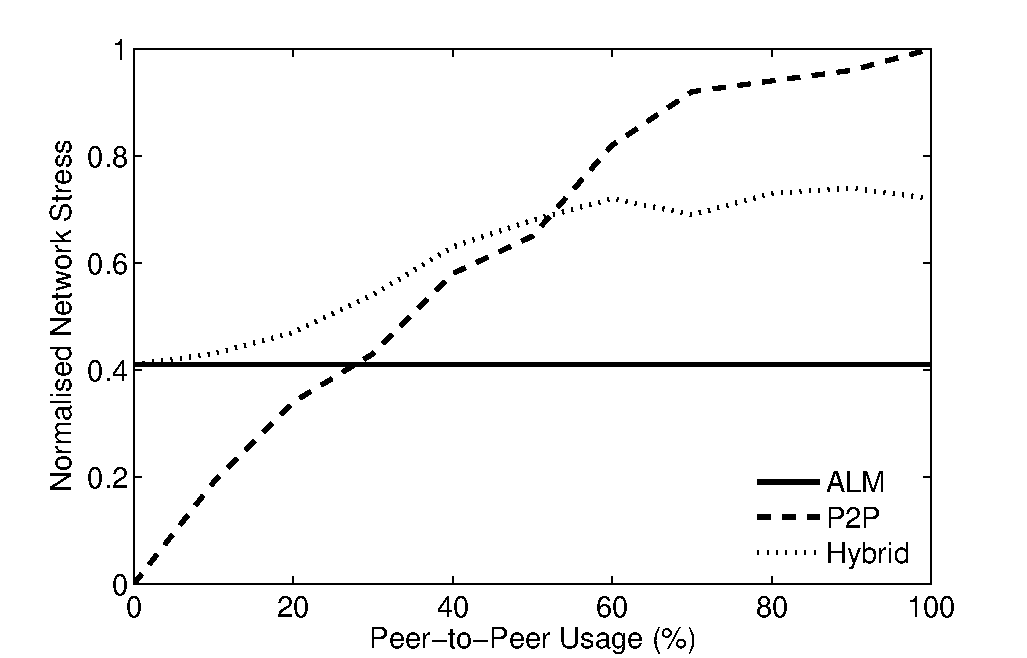
\includegraphics[width=0.5\columnwidth]{./graphs/netintpeer}
        \label{fig:netintpeer}
    }
    \subfloat[][Delivery of a start-to-finish workload] {
        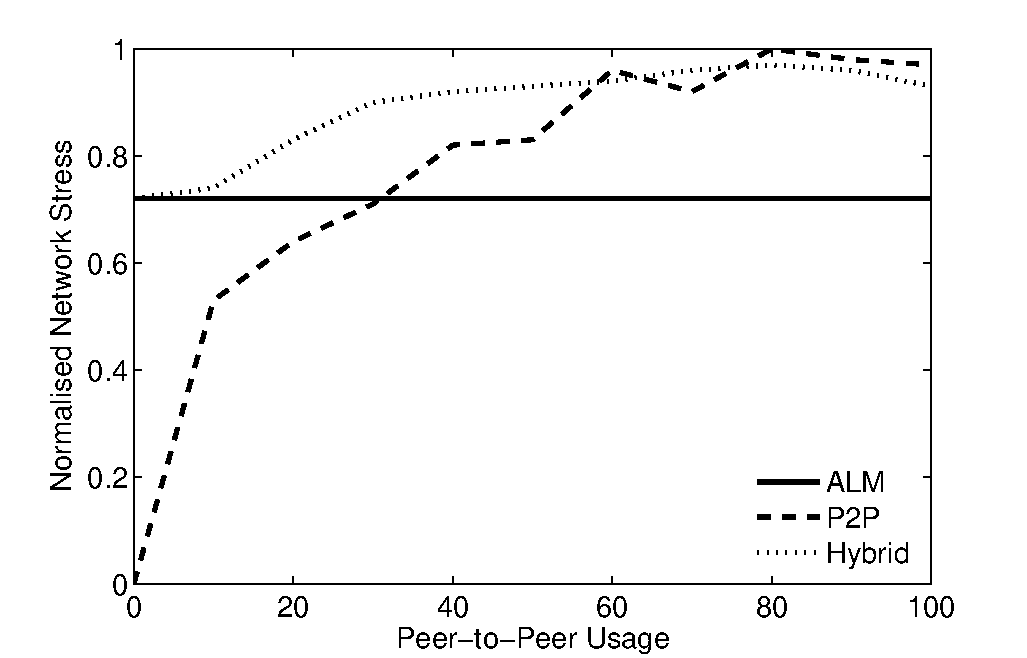
\includegraphics[width=0.5\columnwidth]{./graphs/netstfpeer}
        \label{fig:netstfpeer}
    }
    \caption{Network cost of delivery with varied peer-to-peer size}
\end{figure}

\begin{figure}[t]
    \centering

    \subfloat[][Delivery of an interactive workload] {
        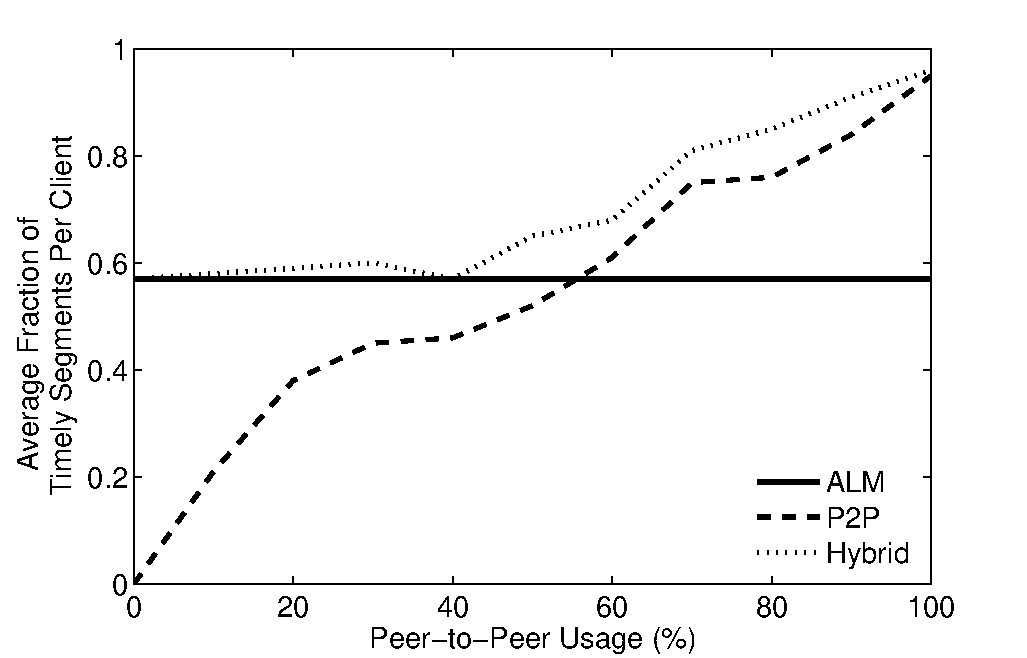
\includegraphics[width=0.5\columnwidth]{./graphs/userintpeer}
        \label{fig:userintpeer}
    }
    \subfloat[][Delivery of a start-to-finish workload] {
        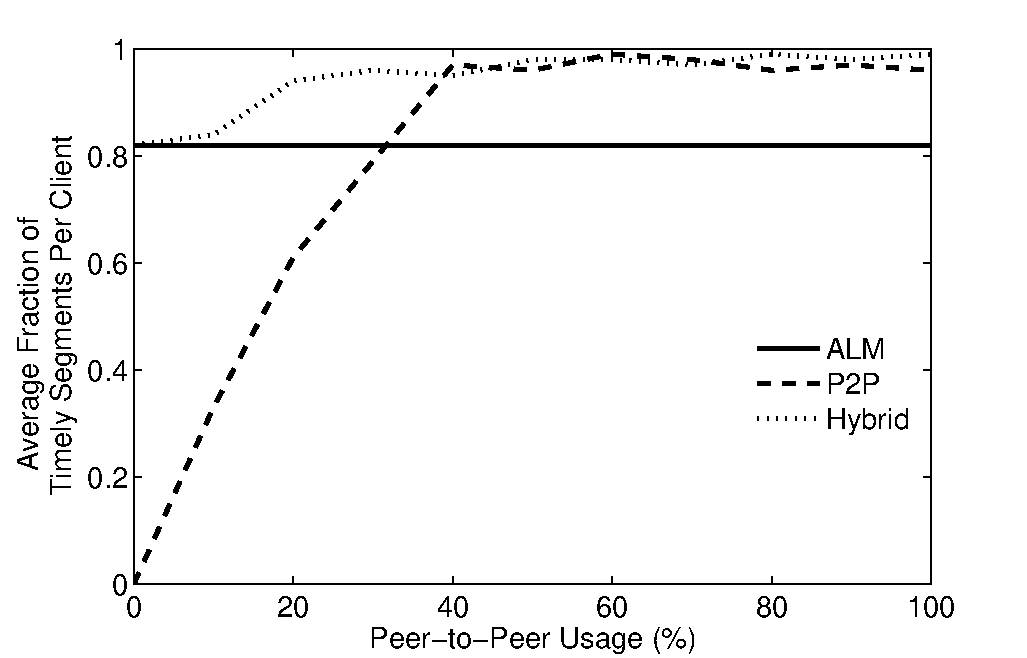
\includegraphics[width=0.5\columnwidth]{./graphs/userstfpeer}
        \label{fig:userstfpeer}
    }
    \caption{User satisfaction during delivery with varied peer-to-peer size}
\end{figure}

\autoref{fig:netintpeer} shows the network stress in terms of data delivered per link for an interactive workload, normalised to the `worst case' of full peer-to-peer usage. As simulations run to the point where clients no longer have any interest in receiving segments, the reduced traffic in the low usage scenarios for the peer-to-peer case is to be expected. Two notable points on this plot are around 25\% and 50\% peer-to-peer usage, where the pull method crosses over the ALM and hybrid approaches respectively. Following the latter intersection, the hybrid method appears to level off while pull P2P continues to increase. Dependent on the user satisfaction for these schemes at these points, this indicates that the hybrid method can produce a consistently lower amount of network traffic relative to push P2P, although the addition of patching is resulting in twice the amount produced by ALM alone. A key point to consider regarding the high network cost of pull P2P is that the ALM-based approach is exploiting the concept of locality in building shortest-path trees to the highly provisioned content nodes. In the pull peer-to-peer case, this does not happen, and many segments are likely being sent lengthy distances between groups of clients viewing the same section of video, potentially across multiple network transit/stub domains.

If the first figures are considered as showing network cost, then the likes of \autoref{fig:userintpeer} show the resultant level of `user satisfaction', in terms of the average fraction of timely segments per client. Recall that two particular points of interest in \autoref{fig:netintpeer} were around the 25\% and 50\% peer-to-peer usage marks. In this figure, however, no significant improvement over pure ALM is shown until around the latter of these points: the 50\--60\% mark. It therefore seems that without the ability to disseminate a large amount of P2P data, the use of the pull P2P approach just results in additional overhead for this type of workload. As the usage increases beyond this point, however, the number of timely segments being delivered increases significantly for both the schemes that make use of P2P. In almost all cases, however, the hybrid method outperforms pull P2P, although not by a large amount. This may be due to the sequential nature of the media playback -- when periodic broadcast is used, most of the data that clients need will be pushed to them anyway -- the pull approach may only be particularly useful when clients have to seek to new points in the media. The high level of interactivity in the workload used for this particular figure may therefore explain the relatively poor performance of pure ALM.

\autoref{fig:netstfpeer} shows the result of a simulation similar to that conducted for \autoref{fig:netintpeer}, but with users consuming the content `start-to-finish'. The network cost is found to be closer between the three methods in this case than with a high-interactivity workload, supporting the idea that user interactivity can be more costly for certain delivery methods. Interestingly, when examined in conjunction with \autoref{fig:userintpeer}, it can be observed that the pull P2P approach outperforms the hybrid method under these metrics when ``peer-to-peer usage'' is around the 40\% mark. This particular simulation result may therefore run contrary to the initial expectation that periodic broadcast may be better suited than pull P2P for many users viewing the media in a generally sequential fashion. Also note, however, that the average fraction of timely segments for pure periodic broadcast in this low-interactivity scenario is significantly better; effectively double that of the high-interactivity workload, and more akin to the results obtained for the high-interactivity workload with small group sizes. This result is as expected, as reduced interactivity correspondingly results in fewer clients jumping between broadcast trees, fewer setup delays, and thus fewer untimely segments according to the clients' demands.

\subsubsection{Additional Nodes}

\begin{figure}[t]
    \centering

    \subfloat[][Additional shared-content] {
        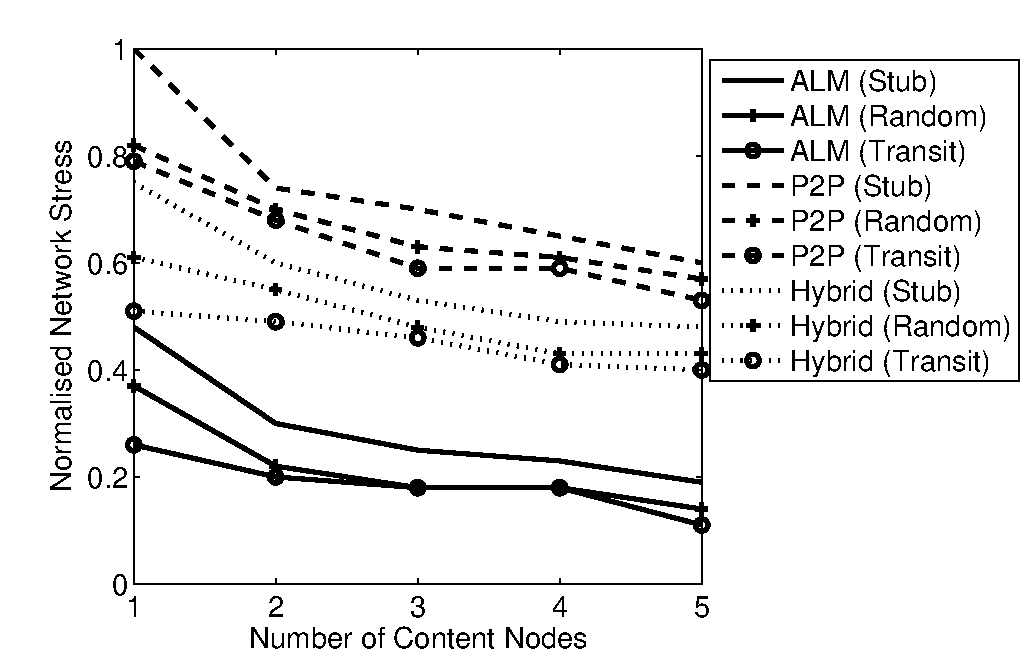
\includegraphics[width=0.5\columnwidth]{./graphs/nodeshared}
        \label{fig:nodeshared}
    }
    \subfloat[][Additional redundant-content nodes] {
        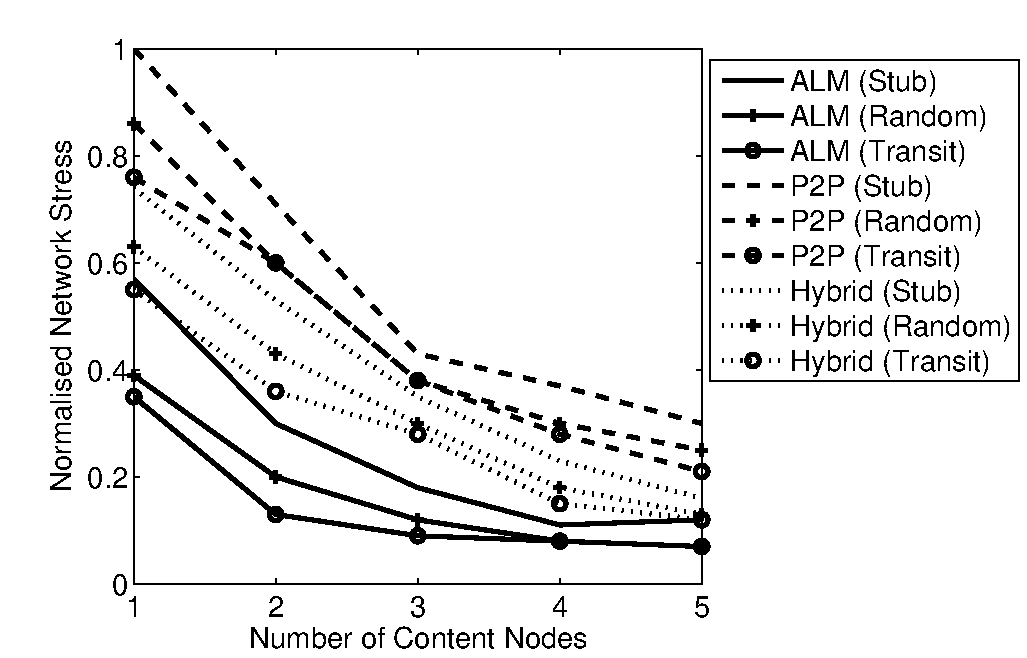
\includegraphics[width=0.5\columnwidth]{./graphs/noderedundant}
        \label{fig:noderedundant}
    }
    \caption{Effect of additional nodes on overall network stress}
\end{figure}

In all cases, as shown in \autoref{fig:nodeshared} and \autoref{fig:noderedundant}, the addition of extra resources in the form of additional content sources (\emph{i.e.}, the roots of trees or seeds in swarms) is beneficial, with similar trends observed regardless of the delivery method being used. This is especially true of the case when content is made available in a redundant fashion rather than simply being `striped' across nodes. The exact placement of these nodes also has some impact, albeit a less significant one, with a slightly diminishing effect as more nodes are made available.

\subsubsection{Key Observations}

From these findings, several points become clear. Regarding network costs in terms of traffic generated, pull P2P is relatively expensive in comparison with the simpler ALM approach. This cost is offset, however, by a resilience to large group sizes and high levels of interactivity in comparison with ALM. Fortunately, when the methods are combined into the hybrid method, network cost is lower than the pull peer-to-peer case, albeit higher than ALM alone, making it an effective compromise. In all cases, larger group sizes result in an increase in the amount of network traffic, and this also has a slightly negative effect on segment utility.

In terms of user satisfaction, larger groups have little effect on the fraction of timely segments received when the peer-to-peer system is involved under any level of interactivity. This is also largely true for the case of pure ALM when low levels of user interactivity are observed, but when users begin to jump around within a video, ALM performs significantly worse. This effect can be attributed to the lengthy join delays when the broadcast trees are particularly long, coupled with the standard waiting period on the broadcast channel to receive the segment(s) the user requires. Naturally, this does not affect the pull approach of the peer-to-peer method, and when this is combined with the ALM scheme, the peer-to-peer system acts as a means of patching; providing the media segments required in an on-demand fashion until the push scheme has stabilised. For similar reasons, segment utility is quite similar across all methods for low interactivity workloads, but when high levels of interactivity occur, there is a marked difference between the schemes. For instance, while the peer-to-peer approach typically achieves high-levels of user satisfaction, a larger percentage of segments are wasted relative to ALM. The naturally sequential nature of the broadcast over ALM may therefore be acting in its favour here, given that users are highly likely to want large numbers of media segments delivered in this fashion.

\subsection{Conclusion}

From the results observed, we can conclude that while peer-to-peer methodologies are certainly feasible for the delivery of interactive content from the user perspective, they are somewhat network-intensive. In contrast, a more traditional approach based around classical periodic broadcast techniques over an application-level multicast structure apparently work well for smaller numbers of passive viewers, but encounters problems when user interactivity and group size increase. The combination of these two approaches, broadly pull and push, can, however, offer a good compromise that provides adaptability to varying conditions in terms of audience size, interactivity levels, and the resources available. Across all the delivery methods considered, providing additional resources in terms of extra content nodes is beneficial, with their placement relative to clients being increasingly important dependent on their abundance.

It is therefore apparent that mixing a live distribution approach such as application-level multicast with an appropriate peer-to-peer patching mechanism over a typical network infrastructure (\emph{i.e.}, typically lacking in IP multicast support) can provide a workable solution for delivery of on-demand video with interactivity support in a CDN environment. Given the wide variety of possible workloads, delivery methods and variables, much potential exists for future work in this field.


    \chapter{Conclusion}
\label{chap:conclusion}

This chapter is divided into three main sections, firstly, a brief overview of contributions this thesis has made. Followed by a discussion of possible future work, and finally wrapped-up with concluding remarks.

\section{Thesis Contributions}

%here
    This thesis has provided several contributions for the research community. For the first time, traces are now available from a highly interactive video-on-demand system, which show behaviour not previously observed. These traces have been analysed and modelled, to produce detailed and thorough user workloads, which will aid in the designing and testing of future video-on-demand techniques.

    Additionally, the modelled behaviour exhibited usage patterns which were a complete departure from the classic start-to-finish models. When users are given a choice and the media is of an appropriate genre, users will only seek to and view the areas they are interested in. This is aided by the bookmark feature, which clearly influenced what was viewed. The combination of this produced \emph{hotspots}, areas of high interest, which were common to all our videos.

    With the models outlined in \autoref{chap:evaluation}, it is clear that many existing delivery techniques do not perform well any more, as they were originally designed under the assumption of the start-to-finish model. However, with these new models it is possible to create new techniques which exploit these new usage patterns. Three new techniques were explained in \autoref{chap:new_techiques}.  These include a method for detecting and moving ill-placed bookmarks, a method to pre-fetch far ahead of playback to popular segments, and finally, a new hybrid scheme which shows how peer-to-peer schemes operate under high interactivity.

    The pre-fetching schemes builds up knowledge in real-time from the live system of what segments of the media are popular and in what order they are typically viewed. Using this knowledge it was demonstrated that users can successfully pre-fetch segments or \emph{hotspots}, which they will probably view in the near future.

    The hybrid peer-to-peer section outlined how existing peer-to-peer solutions were not appropriate for these interactive workload. This is supported by our experimentation which shows that a hybrid push/pull approach performed far better than existing peer-to-peer approaches.

%
%\begin{itemize}
%    \item Detailed Analysis of a highly interactive Video-on-demand system, now available to the research community
%    \item Models of how users interactive with the media
%        \item Observed patterns previous not seen
%            \item People do not consume start-to-finish
%            \item Bookmarks highly influence things
%            \item Hotspots are common
%
%    \item With these models we can start producing new techniques to exploit these behaviour
%    \begin{itemize}
%       \item Sequences of events (encouraging to be predictable)
%       \item Moving the bookmarks
%       \item Predicting the sequences of events
%       \item Hybrid delivery mechanisms. How both push and pull can be used to provide efficient delivery, whilst catering for highly dynamic workloads
%    \end{itemize}
%\end{itemize}

\section{Future Work}

    As bookmarks in our system were very popular, in a fully autonomic system the bookmarks should perhaps be created automatically. This could occur after the system has detected a large number of requests for a specific area of a video. A bookmark could then be provisionally placed and its position refined by a bookmark-moving algorithm.

    Hotspots should also be detected automatically by the system, as their position and popularity can greatly be exploited. In this thesis we have only discussed the hotspot's length, but equally their start position can be inferred in the same (or similar) way to a bookmark's position. Alternative approaches could be taken which, for example, rank all the segments of the media by their popularity, and decide the top-N\% should be hotspots. These rankings could easily be obtained using a cache replacement policy such as the least frequently used (LFU) or least recently used (LRU).

    During our experiment, users were unhappy that we ``spoilt the experience'' of watching the sporting events covered somewhat, as the user could quickly determine the final outcome of the event from the bookmark names. The suggestion was made that we avoid labelling the bookmarks and instead simply describe them as points of interest. This could equally work if the bookmarks were autonomically created, since a system would be unable to name them itself. Note, unnamed bookmarks would only be useful if they are typically accessed sequentially, and not based on their name alone.

    It was shown that pre-fetched bookmark hotspots only covered 35\% of all viewed segments. Thus, pre-fetching schemes should consider more segments. This, of course, would make it harder to decide which segments to pre-fetch next. The cost of making a wrong decision could be reduced if the pre-fetching technique was modified, for example, pre-fetching more than one choice simultaneously.

    Additionally, the data required for pre-fetching has not been fully exploited. There are numerous other uses for this data, such as producing management or business reports, better caching algorithms, construction of peer-to-peer overlays, or even deciding which segments to push to the user overnight. The cache algorithm could, for example, take into account any segments of the video which depend on another segment, and thus related segments are kept or evicted from the cache together.  With peer-to-peer overlays, the network topology could fundamentally be structured based on the pre-fetching knowledge.

    This thesis briefly looked at peer-to-peer delivery and it is clear that as demand for online media increases, techniques such as P2P will be used more. Many internet service providers (ISPs) are worried about P2P, as their networks were not designed or deployed to be symmetric. The typical home broadband connection has a higher downstream bitrate than upstream making it asymmetric. Yet, it has been shown that if the P2P topology is designed correctly, it can reduce the cost for the ISPs and content providers, with only a minor decrease in performance for the users~\cite{karagiannis2005sis,huang2007civ}. This still needs further work to help balance the cost to ISPs, and the performance impact to the user, especially when considering the highly interactive workloads.

    Many of the suggested solutions for delivering this content, such as peer-to-peer, are relatively simple for a standard desktop PC to use, however, more and more media is being consumed via mobile devices. 3G phones are being used to watch clips from the internet and Apple iPods are automatically downloading audio and video podcasts each day, providing their users with a ``personal on demand broadcasting'' service. These small mobile devices may not benefit from client-side improvements; instead the network should perhaps become more intelligent to be able to serve this new generation of device.

    While not available today, future forms of interactivity may add an extra dimension to these problems. For example, systems which allow picture-in-picture (PiP), the ability to display one main video, with one or more smaller supplementary videos being displayed on top. Imagine a system where when watching a programme, areas of the video could be highlighted to form a hyperlink to more information. This hyperlinked information would then be displayed with picture-in-picture technology. This can be considered useful in many situations, for example, finding statistics about players in sporting events, viewing more information on a news article, or reading reviews or production notes about a film currently being shown. Now, videos could hyperlink between each other, not just causing links between \emph{hotspots}, but now between videos.

    While not the case for all content, high levels of interactivity are becoming more common, whilst users are both relying on and expecting video-on-demand services to provide more advanced interactive functionality. Our study suggests that CDN mechanisms must improve to handle more diverse applications, content and users. To achieve this, the development of new algorithms must be driven by models derived from realistic characterised workloads. The development of such strategies is reliant on gaining a deeper understanding of the relevant workload parameters. The analysis and models presented in this thesis aim to aid in this endeavour.

\section{Conclusion}

%\begin{itemize}
%    \item Detailed Analysis of a highly interactive Video-on-demand system
%    \begin{itemize}
%        \item Observed patterns previous not seen
%            \item Bookmarks highly influence things
%        \item People do not consume start-to-finish
%            \item Hotspots are common
%        \item Models of how users interactive with the media
%        \item Sequences of events (encouraging to be predictable)
%    \end{itemize}
%    \item With these models we can start producing new techniques to exploit these behaviour
%    \begin{itemize}
%       \item Moving the bookmarks
%       \item Predicting the sequences of events
%       \item Hybrid delivery mechanisms. How both push and pull can be used to provide efficient delivery, whilst catering for highly dynamic workloads
%    \end{itemize}
%\end{itemize}

    We have presented a study and characterisation of user behaviour for our interactive Video-on-Demand system. We note that by adding simple bookmarks to points of interest within the media, the access patterns are greatly influenced. This behaviour led to high levels of seeking which created relatively short and sparsely distributed segments whose popularity was orders of magnitude more popular than other segments.

    Many existing delivery mechanisms are not designed for high levels of interactive behaviour and are instead optimised for classic start-to-finish streaming. Content distribution techniques must therefore adapt to efficiently handle these kinds of access patterns. They could, for example, take advantage of the power-law distributions of segment popularity by replicating those that generate the most demand. For instance, we observed that 10\% of segments accounted for 44\% of all requests.

    The departure from classic start-to-finish playback encourages the design of agile delivery mechanisms that allow quick seeking, and expect certain segments to be more popular. We have seen that adding bookmarks will highly influence the order in which users view the content, making the sequence of actions somewhat predictable. This can then be exploited by allowing users to pre-fetch content that they are predicted to need shortly, thus reducing any delays that they are likely to experience. However, we noted that bookmarks could be harmful by causing unnecessary seeks if incorrectly placed. This could be remedied for both client and server by simply moving the bookmark autonomically based on observed user behaviour.

    Advances in pull-based peer-to-peer VoD can aid in agile delivery, however the overheads associated make it unacceptable in some situations. Instead, a combination of push-based peer-to-peer delivery, which typically does not handle seeking well, and pull-based, can produce an efficient delivery platform for these interactive workloads.

    So far we have only considered bookmarks within music and sport videos, but bookmarks are equally applicable in many other genres. For example, bookmarks are commonly found in the form of chapters on video DVDs. It is not clear if the same high levels of interactivity would be observed in such media, or if the classic start-to-finish model would still be prevalent.

    In conclusion, we are entering a new era of video-on-demand, one where media is being consumed in abundance, on a myriad of devices. Our VoD systems must be flexible and agile to support current and future trends, as well as to take advantage of new techniques such as peer-to-peer, or to expect new user behaviours such as those demonstrated in this thesis. Overall, this is an exciting new future for online media, and one which provides many opportunities for improvement.

%\begin{itemize}
%    \item Start investigating how CDNs can take advantage of these concepts. (For instance, we observed that 10\% of segments accounted for 44\% of all requests.)
%    \item Try a lot of these ideas for real. Thus far only been simulated
%    \item Auto creation of bookmarks
%    \item "spoilt the experience", try different bookmark labelling
%    \item Pre-fetching multiple things simultaneously. Pre-fetching all segments, not just bookmarks
%    \item Investigate how pre-fetching knowledge could be used more. Management reports, better caching, better construction of p2p overlays. Pushed out over night
%    \item Pre-fetching requires disk space, what about mobile devices?
%    \item Can a user on a phone even seek?!
%    \item Pre-fetching between videos
%\end{itemize}
%
%\section{Summary}


\backmatter
    \chapter{Appendix}
\singlespacing
    % Configs what the back references look like
\renewcommand*{\backref}[1]{}
\renewcommand*{\backrefalt}[4]{%
    \ifcase #1 %
        [Never cited]%
    \or
        [Cited on page #2]%
    \else
        [Cited on pages #2]%
    \fi
}%

% ************************** Bib Styles ********************************
\bibliographystyle{alpha} % [AA08] Ordered by author's name
%\bibliographystyle{plain} % [1] Ordered by author's name
%\bibliographystyle{abbrv} % same as plain but with less info in bib
%\bibliographystyle{unsrt} % [1] Ordered by first use


%\todo{Make sure nocite is removed}
%\nocite{*}
\phantomsection
\addcontentsline{toc}{chapter}{\bibname}
\bibliography{bib}


\end{document}
